\PassOptionsToPackage{dvipsnames}{xcolor}
% **************************************************
% Document Class Definition
% **************************************************
\documentclass[%
    paper=A4,               % paper size --> A4 is default in Germany
    twoside=true,           % onesite or twoside printing
    openright,              % doublepage cleaning ends up right side
    parskip=half,           % spacing value / method for paragraphs
    chapterprefix=true,     % prefix for chapter marks
    11pt,                   % font size
    headings=normal,        % size of headings
    bibliography=totoc,     % include bib in toc
    listof=totoc,           % include listof entries in toc
    titlepage=on,           % own page for each title page
    captions=tableabove,    % display table captions above the float env
    chapterprefix=false,    % do not display a prefix for chapters
    appendixprefix=false,   % but display a prefix for appendix chapter
    draft=false,            % value for draft version
]{scrreprt}%

% **************************************************
% Setup YOUR thesis document in this file !
% **************************************************
% !TEX root = main.tex


% **************************************************
% Files' Character Encoding
% **************************************************
\PassOptionsToPackage{utf8}{inputenc}
\usepackage{inputenc}

% **************************************************
% PDF annotation
% **************************************************
\usepackage[author={Auteur1}]{pdfcomment}
\newcommand{\chl}[2]{\pdfmarkupcomment[markup=Highlight, color=red!20]{#1}{#2}}

%%% Main Env %%%
\newcommand{\rSPS}{\textit{RA-SPS}}
\newcommand{\pSPS}{\textit{PA-SPS}}

% **************************************************
% Information and Commands for Reuse
% **************************************************
\newcommand{\thesisTitle}{Dynamic adaptation in Stream Processing Systems}

\newcommand{\thesisName}{Daniel Wladdimiro Cottet}
\newcommand{\thesisSubject}{Distributed Systems}

\newcommand{\thesisDate}{8 Janvier 2024}
\newcommand{\thesisVersion}{Review Version}

\newcommand{\thesisFirstReviewer}{Reviewer1 Name}
\newcommand{\thesisFirstReviewerUniversity}{\protect{Université Paris-Sorbonne}}
%\newcommand{\thesisFirstReviewerDepartment}{Department of Clean Thesis Style}

\newcommand{\thesisSecondReviewer}{Reviewer2 Name}
\newcommand{\thesisSecondReviewerUniversity}{\protect{Université Pierre et Marie Curie}}
%\newcommand{\thesisSecondReviewerDepartment}{Department of Clean Thesis Style}

\newcommand{\thesisFirstSupervisor}{Jean-Mich Directeur}
\newcommand{\thesisSecondSupervisor}{Jean-Mich Encadrant}

\newcommand{\thesisUniversity}{\protect{Sorbonne Université}}
\newcommand{\thesisUniversityDepartment}{Laboratoire d'Informatique de Paris 6}
%\newcommand{\thesisUniversityInstitute}{Institute for Clean Thesis Dev}
\newcommand{\thesisUniversityGroup}{DELYS team}
\newcommand{\thesisUniversityCity}{Paris}
%\newcommand{\thesisUniversityStreetAddress}{Street address}
%\newcommand{\thesisUniversityPostalCode}{Postal Code}


% **************************************************
% Debug LaTeX Information
% **************************************************
%\listfiles


% **************************************************
% Other Packages
% **************************************************
\usepackage{morewrites}
\usepackage[pass]{geometry}
\usepackage{scrhack}
\usepackage{listings}
\usepackage{tikz}
\usetikzlibrary{shapes.misc, shapes.geometric, positioning, arrows.meta, calc, arrows}
%\usepackage{xcolor}
% I'm not using glossaries, so I commented both next lines
% \usepackage[nopostdot,toc,acronym]{glossaries}
% \makeglossaries
\usepackage{import}
\usepackage[most]{tcolorbox}
\tcbuselibrary{listings}
\usepackage{amssymb}
\usepackage{caption}
\usepackage{subcaption}
\usepackage{adjustbox}
\usepackage{colortbl}
\usepackage{placeins}[section, below]
\usepackage{hyperref}
\usepackage{macros}
\usepackage[defblank]{paralist}  %% inline lists
\usepackage[inline,shortlabels]{enumitem} % must come just after paralist!
\usepackage{wrapfig}

% **************************************************
% Load and Configure Packages
% **************************************************
% cSpell: disable
\usepackage[english]{babel} % babel system, adjust the language of the content
\PassOptionsToPackage{% setup clean thesis style
    figuresep=colon,%
    hangfigurecaption=false,%
    hangsection=true,%
    hangsubsection=true,%
    sansserif=false,%
    configurelistings=true,%
    colorize=full,%
%    colorize=bw,%
    colortheme=bluemagenta,%
    configurebiblatex=true,%
    bibsys=bibtex,%
    bibfile=main,%
    bibstyle=alphabetic,%
    bibsorting=nty,%
}{cleanthesis}
\usepackage{cleanthesis}

\hypersetup{% setup the hyperref-package options
    pdftitle={\thesisTitle},    %   - title (PDF meta)
    pdfsubject={\thesisSubject},%   - subject (PDF meta)
    pdfauthor={\thesisName},    %   - author (PDF meta)
    plainpages=false,           %   -
    colorlinks=false,           %   - colorize links?
    pdfborder={0 0 0},          %   -
    breaklinks=true,            %   - allow line break inside links
    bookmarksnumbered=true,     %
    bookmarksopen=true          %
}

% Nicer color
\definecolor{red}{HTML}{9B0000}
\definecolor{lightred}{HTML}{FF5131}
\definecolor{green}{HTML}{1FAA00}
\definecolor{lightgreen}{HTML}{9CFF57}
\definecolor{purple}{HTML}{7200CA}
\definecolor{blue}{HTML}{0064B7}
\definecolor{verylightgrey}{HTML}{F1F1F1}
\colorlet{ctcolorfootertitlelight}{ctcolorfootertitle!20}

\lstdefinelanguage{diff}{
% basicstyle=\ttfamily\bfseries\footnotesize,
  morecomment=[f][\color{blue}]{@},
  morecomment=[f][\color{green}]{+},
  morecomment=[f][\color{red}]{-},
  keepspaces=true,
  identifierstyle=\color{black},
}

\lstdefinelanguage{spdiff}{
% basicstyle=\ttfamily\bfseries\footnotesize,
  morecomment=[s][\color{blue}]{@@}{@@},
  morecomment=[s][\color{blue}]{@rule1@}{@@},
  morecomment=[s][\color{blue}]{@rule2@}{@@},
  morecomment=[f][\color{green}]{+},
  morecomment=[f][\color{red}]{-},
  morekeywords={expression},
  morekeywords={identifier},
  keepspaces=true,
  identifierstyle=\color{black},
}

\newtcolorbox{notice}[1][]{enhanced,
  before skip=3mm,after skip=7mm,
  boxrule=0pt,left=7mm,right=2mm,top=1mm,bottom=1mm,
  colback=ctcolorfootertitlelight,
  sharp corners,
  frame hidden,
  underlay={%
    \path[fill=ctcolorfootertitle,draw=none] (interior.south west) rectangle node[white]{\huge\bfseries !} ([xshift=6mm]interior.north west);
    },
  #1}


\newtcblisting{namedlisting}[2][]{%
  enhanced,
  sharp corners,
  frame hidden,
  boxsep=0pt,
  title={\hspace*{3.5mm}#2},
  titlerule=0pt,
  colbacktitle=ctcolormain!20,
  coltitle=black,
  toptitle=1mm,
  bottomtitle=1mm,
  listing only,
  left=0pt,
  top=0pt,
  bottom=0pt,
  right=0pt,
  toprule=0pt,
  leftrule=0pt,
  bottomrule=0pt,
  rightrule=0pt,
  colframe=ctcolormain,
  listing options={aboveskip=0pt, belowskip=0pt, #1},
}

\tikzset{%
  >=latex,
  edge/.style={
    ->,
    rounded corners=3pt
  },
  node/.style={%
    rectangle,
    rounded corners=1pt,
    draw,
    thick,
    fill=ctcolorgraylighter,
    minimum height=1.5em,
  },
  empty/.style={%
    minimum height=0,
  },
  removed/.style={
    text=red,
    draw=red,
  },
  added/.style={
    text=green,
    draw=green,
  },
  fake/.style={
    densely dotted,
    text=ctcolorgray,
  },
  special/.style={
    trapezium,
    trapezium left angle=60,
    trapezium right angle=120,
    minimum width=2cm,
  },
  entry port/.style={
    alias=this,
    append after command={%
      \pgfextra
        \draw[-(, thick] (this) -- ($(this.north) + (0, 0.25)$);
      \endpgfextra
    },
  },
  exit port/.style={
    alias=this,
    append after command={%
      \pgfextra
        \draw[-o, thick] (this) -- ($(this.south) + (0, -0.35)$);
      \endpgfextra
    },
  },
}
% cSpell: enable

% ***********
% Here you can add your own commands 
% ***********
\newcommand{\etal}{\textit{et al.}}

\newcommand\norm[1]{\left\lVert#1\right\rVert}

\newcommand{\hlcell}[1]{\cellcolor{ctcolorfootertitle} \textcolor{white}{\textbf{#1}}}
\newcommand{\hlrow}{\rowcolor{ctcolorfootertitle} \color{white} \bfseries}

\renewcommand{\arraystretch}{1.2} % fat table

\newcommand{\bfemph}[1]{\textbf{\textit{#1}}}
%\usepackage{algorithm,algorithmic}

% **************************************************
% Document CONTENT
% **************************************************
\begin{document}

% uncomment the following command to fill up pages with
% whitespace instead of aligning the first and last lines
% of a page (see \raggedbottom vs. \flushbottom)
%\raggedbottom

% --------------------------
% rename document parts
% --------------------------

% > set short label names for floating environments figure and table
\renewcaptionname{english}{\figurename}{Fig.}
\renewcaptionname{english}{\tablename}{Tab.}

% > rename the title of the LOL, i.e. list of listings (default is "Listings")
\renewcommand*{\lstlistlistingname}{List of Listings}

% --------------------------
% Front matter
% --------------------------
\pagenumbering{roman}			% roman page numbing (invisible for empty page style)
%% Uncomment below commands if you want the arabic numbering to include Front pages
%% This is only useful if you are a literature student.
% \pagestyle{empty}				% no header or footers
% \pagenumbering{arabic}			% arabic page numbering
% \setcounter{page}{1}			% set page counter

% !TEX root = ../main.tex
%
% ------------------------------------  --> cover title page

\newcommand{\jurymember}[5]{\hspace{1.5em}\textbf{{#1} \textsc{{#2}}}, {#3}, {#4} \hfill \textit{{#5}}\\}

\newgeometry{left=2.8cm, right=2.5cm, top=2cm, bottom=2cm}
\begin{titlepage}
	\pdfbookmark[0]{Cover}{Cover}
	\begin{flushleft}
      
\includegraphics[height=1.7cm]{figures/sorbonne.pdf}
      \hfill
	  % TODO: replace with your Lab logo
      
\includegraphics[height=1.7cm]{figures/LogoLIP6.pdf}
      \hfill
	  % TODO: replace with your Team logo
      %\includegraphics[height=1.7cm]{figures/inria.pdf}
	  % TODO: you may add your company logo if you are a CIFRE PhD Student
	  % \hfill
      % \includegraphics[height=1.7cm]{figures/cifre-logo.pdf}
	\end{flushleft}
	\vfill
	\begin{center}
        \vspace{1em}
        {\large Thèse présentée pour l'obtention du grade de}\\
        \vspace{1em}
        {\LARGE DOCTEUR de SORBONNE UNIVERSITÉ}\\
        \vspace{2em}
		{\small Spécialité}\\
		\vspace{0.5em}
		% TODO: specialty of the doctoral school, this is the one that will appear in the diploma
		{\Large Ingénierie / Systèmes Informatiques}\\
		\vspace{2em}
        {\large École doctorale}\\
		\vspace{0.5em}
		{\Large Informatique, Télécommunication et Électronique Paris (ED130)}\\
    \end{center}
	\vfill
	\begin{flushright}
	\hfill
	\vfill
	{\LARGE\thesisTitle \par}
	\rule[5pt]{\textwidth}{.4pt} \par
	{\Large\thesisName}
	\vfill
	\end{flushright}
	%% TODO: If final version:
	Soutenue publiquement le : \textit{\large\thesisDate}
	%% Else, for review version:
	% Version: \thesisVersion
	\begin{flushleft}
		Devant un jury composé de :\\
		% TODO: jury members should follow two orders:
		%% 1- Role: Reviewer -> Jury -> Guest -> Advisor
		%% 2- For each role, alphabetical order
		%\jurymember{Prénom}{Nom}{Poste}{Université}{Role dans le jury}
		\jurymember{Fabrice}{Huet}{Professeur}{Univ. Nice Sophia Antipolis, CNRS, I3S, UMR 7271}{Rapporteur}
		\jurymember{Cédric}{Tedeschi}{Professeur}{Université Rennes 1, IRISA}{Rapporteur}
		\jurymember{Nicolás}{Hidalgo}{Maîtres de conférences}{Universidad Diego Portales}{Examinateur}
		\jurymember{Sébastien}{Monnet}{Professeur}{Université Savoie Mont Blanc - \textit{Président}}{Examinateur}
		\jurymember{Luciana}{Arantes}{Maîtres de conférences}{Sorbonne Université, LIP6}{Co-Encadrante}
		\jurymember{Pierre}{Sens}{Professeur}{Sorbonne Université, LIP6}{Directeur de thèse}
	\end{flushleft}
\end{titlepage}
\restoregeometry
 % INCLUDE: all titlepages
\clearpage
\vfill
\begin{flushright}
    \vfill
	\hfill
	\emph{Es el canto universal\\Cadena que hará triunfar\\El derecho de vivir en paz}
	\vfill
\end{flushright}
\mbox{}
\vfill
\begin{wrapfigure}{L}{0.25\textwidth}
    \begin{center}
        \vspace{-\baselineskip}
        
\includegraphics[width=0.25\textwidth]{figures/thesis-copyright.png}
    \end{center}
\end{wrapfigure}
\noindent
\textbf{Copyright:}\\
Except where otherwise noted,
this work is licensed under\\
\textbf{https://creativecommons.org/licenses/by-nc-nd/4.0/} % INCLUDE: Sorbonne Univ Thesis Copyright
\cleardoublepage

\pagestyle{plain}				% display just page numbers
%
% !TEX root = ../main.tex
%
\pdfbookmark[0]{Remerciements}{Remerciements}
\addchap*{Remerciements}

The first thing I would like to say is: \textit{Gracias a la vida, que me ha dado tanto}. I am thankful to have closed this cycle of my life, from which I have learned both professionally and personally. I am thankful to have been surrounded by wonderful people, who gave me the energy to move forward. I am thankful to have lived long enough to be here and to be able to look at the sky. I thank you from the bottom of my heart.

I would like to thank my teachers, I feel very fortunate to have worked with you. Pierre, I thank you for all the confidence you have had in my project, my ideas, and my goals. Without your support I could not have come this far, and it is partly thanks to you. Merci beaucoup. Luciana, I thank you for all the love and dedication you have shown me, I will never forget all those details. Without your welcome my Latin heart would be colder, and with you I have felt this warmth that makes me feel at home. Muito obrigado. I would also like to thank Nicolás, because you have been an important person in this journey. Without you, this cycle could not have started, and likewise, it could not have ended. So many conversations we had, which gave me the strength to keep going when I felt stuck. Muchas gracias.

I would like to thank everyone who welcomed me at the Sorbonne Université, because each one contributed to the progress of this journey. So many people who trusted me to start on my teaching path, who gave me the wings to begin a great challenge. Thank you so much.

I would like to thank everyone who has welcomed me in Paris. Although many people come and go, each one will have a part of my heart, and I am grateful for the love they have given me. Without these people, everything would be more difficult.

I would like to thank my family. Alba, quién sabe en qué momento de tu vida estés leyendo esto o probablemente ya te lo habré leído, pero quiero que sepas lo agradecido y orgulloso que estoy de ser tu papá, has sido una hija maravillosa, quién me ha brindado su amor incondicional. Cami, te quiero agradecer por haber emprendido este viaje a mi lado, has sido una de las grandes artífices de esta aventura, la cual ha culminado gracias al cariño y apoyo que me has dado, sin dudas todo sería distinto sin ti. Papá, te quiero agradecer todo el apoyo y confianza que has tenido conmigo, desde que emprendí este viaje siento que hemos pasado un período maravilloso juntos. Sofi, Amandi, Iñaki y Victor, gracias por todo el cariño vertido todas las veces que los visito en nuestra querida patria. Mamá, ya no puedo agradecerte, lamentablemente ya no estás acá, pero te dedico estas palabras de agradecimiento por haberme hecho quién soy. Gracias totales, les amo con todo mi corazón.

Thanks to the Chilean government. This thesis was funded by the National Agency for Research and Development National Agency for Research and Development (ANID) / Scholarship Program / DOCTORADO BECAS CHILE / 2018 - 72190551. I want to thank the project ANID FONDECYT Nº11190314, Chile. This material is based upon work supported by the Google Cloud Research Credits program with the award GCP19980904. % INCLUDE: acknowledgement
\cleardoublepage
%
% !TEX root = ../main.tex
%
\pdfbookmark[0]{Abstract}{Abstract}
\addchap*{Abstract}
\label{abstract}

The amount of data produced by today's web-based systems and applications increases rapidly, due to the many interactions with users (e.g. real-time stock market transactions, multiplayer games, streaming data produced by Twitter, etc.). As a result, there is a growing demand, particularly in the fields of commerce, security and research, for systems capable of processing this data in real time and providing useful information in a short space of time. Stream processing systems (SPS) meet these needs and have been widely used for this purpose. The aim of SPSs is to process large volumes of data in real time by housing a set of operators in applications based on Directed acyclic graphs (DAG).

Most existing SPSs, such as Flink or Storm, are configured prior to deployment, usually defining the DAG and the number of operator replicas in advance. Overestimating the number of replicas can lead to a waste of allocated resources. On the other hand, depending on interaction with the environment, the rate of input data can fluctuate dynamically and, as a result, operators can become overloaded, leading to a degradation in system performance. These SPSs are not capable of dynamically adapting to operator workload and input rate variations.
One solution to this problem is to dynamically increase the number of resources, physical or logical, allocated to the SPS when the processing demand of one or more operators increases.

This thesis presents two SPSs, \rSPS{} and \pSPS{}, reactive and predictive approach respectively, for dynamically modifying the number of operator replicas. The reactive approach relies on the current state of operators computed on multiple metrics, while the predictive model is based on input rate variation, operator execution time, and queued events. 
The two SPSs extend Storm SPS to dynamically reconfigure the number of copies without having to downtime the application. They also implement a load balancer that distributes incoming events fairly among operator replicas.

Experiments on the Google Cloud Platform (GCP) were carried out with applications that process Twitter data, DNS traffic, or logs traces. Performance was evaluated with different configurations and the results were compared with those of running the same applications on the original Storm as well as with state-of-the-art work such as SPS DABS-Storm, which also adapt the number of replicas. The comparison shows that both \rSPS{} and \pSPS{} can significantly improve the number of events processed, while reducing costs.

\textbf{Keywords:} 
Stream processing, Adaptive SPS, Predictive algorithm, Reactive algorithm, Google Cloud Platform.	% INCLUDE: the abstracts (english)
\clearpage
% !TEX root = ../main.tex
%
\pdfbookmark[0]{Résumé}{Résumé}
\addchap*{Résumé}
\label{chap:résumé}

Le nombre de données produites par les systèmes ou applications Web actuels augmente rapidement en raison des nombreuses interactions avec les utilisateurs (dans le cadre par exemple, transactions boursières en temps réel, des jeux multijoueurs, des données en continu produits par Twitter, etc.). Ainsi, il existe une demande croissante, notamment dans les domaines du commerce, de la sécurité et de la recherche, pour des systèmes capables de traiter ces données en temps réel et de fournir des informations utiles dans un court laps de temps. Les systèmes de traitement des flux (SPS) répondent à ces besoins et ont été largement utilisés à cette fin. L'objectif des SPS est de traiter de grands volumes de données en temps réel en endentent un ensemble d’opérateurs dans des applications structurée en DAG.

Le plupart des SPS existants, tels que Flink ou Storm, sont configurés avant leur déploiement, définissant généralement à l'avance le DAG et le nombre de répliques opérateurs. Une surestimation du nombre de répliques entraîne alors un gaspillage des ressources allouées. D'autre part, en fonction de l'interaction avec l'environnement, le taux de données en entrée peut fluctuer de manière dynamique et, par conséquent, les opérateurs peuvent être surchargés, ce qui entraîne une dégradation des performances du système. Ces SPS ne sont pas capables de s'adapter dynamiquement à la charge de travail de l'opérateur et aux variations du taux d'entrée.
Pour résoudre ce problème, une solution consiste à augmenter dynamiquement le nombre de ressources, physiques ou logiques, allouées au SPS lorsque la demande de traitement d'un ou plusieurs opérateurs augmente.

Nous présentons dans cette thèse deux approches, \rSPS{} et \pSPS{}, pour modifier dynamiquement le nombre de répliques d'un opérateur. L'approche réactive repose sur l’état courant des opérateurs calculé sur de multiples métriques. Tandis que le modèle prédictif se base sur la variation du taux d'entrée, le temps d'exécution des opérateurs et les événements en file d'attente. 
Nous avons également étendu Storm pour reconfigurer dynamiquement le nombre de copies sans avoir à geler l’application. Notre SPS met aussi en œuvre un équilibreur de charge qui distribue les événements entrants de manière équitable entre les répliques d'un opérateur.

Des expériences sur la Google Cloud Platform (GCP) ont été menées avec des applications qui traitent le flux Twitter, le trafic DNS ou les traces de flux du journal système. Nous avons évalué différentes configurations et les avons comparées avec l'implémentation originale de Storm ainsi qu'avec des travaux de pointe tels que SPS DABS-Storm qui adapte également le nombre de répliques. Les résultat montrent que notre approche permet d’améliorer de manière conséquente le nombre d’événement traité tout en réduisant les coûts.

\textbf{Mots-clés:} 
Flux de données, Traitement en temps réel, Algorithme predictive, Algorithme reactive.	% INCLUDE: the abstracts (french)
\cleardoublepage
%
\currentpdfbookmark{\contentsname}{toc}
\setcounter{tocdepth}{2}		% define depth of toc
\tableofcontents				% display table of contents
\cleardoublepage

% --------------------------
% Body matter
% --------------------------
\pagestyle{empty}				% no header or footers
\pagenumbering{arabic}			% arabic page numbering starts from Body
\pagestyle{scrheadings}			% header and footer style

%% Uncomment the following lines using the \part command
%% to add part sections
% !TEX root = ../main.tex
%
\chapter{Introduction}
\label{intro}
The tremendous volume of information in the Internet started with Web 2.0 development. Web 2.0 established a paradigm shift where users actively participate and share data through applications such as blogs, social networks, or other web applications \citep{NEWMAN2016591}. %As time goes by, the information continues to grow at a feared rate, therefore data processing becomes challenging.
Since the amount of exchanged information grows everyday faster, data processing becomes even more challenging.

Figure \ref{fig:web} presents an example of interactions between users and applications, such as uploading or downloading music, commenting on a post, and receiving notifications, among many other possibilities.

\begin{figure}[!ht]
    \centering
    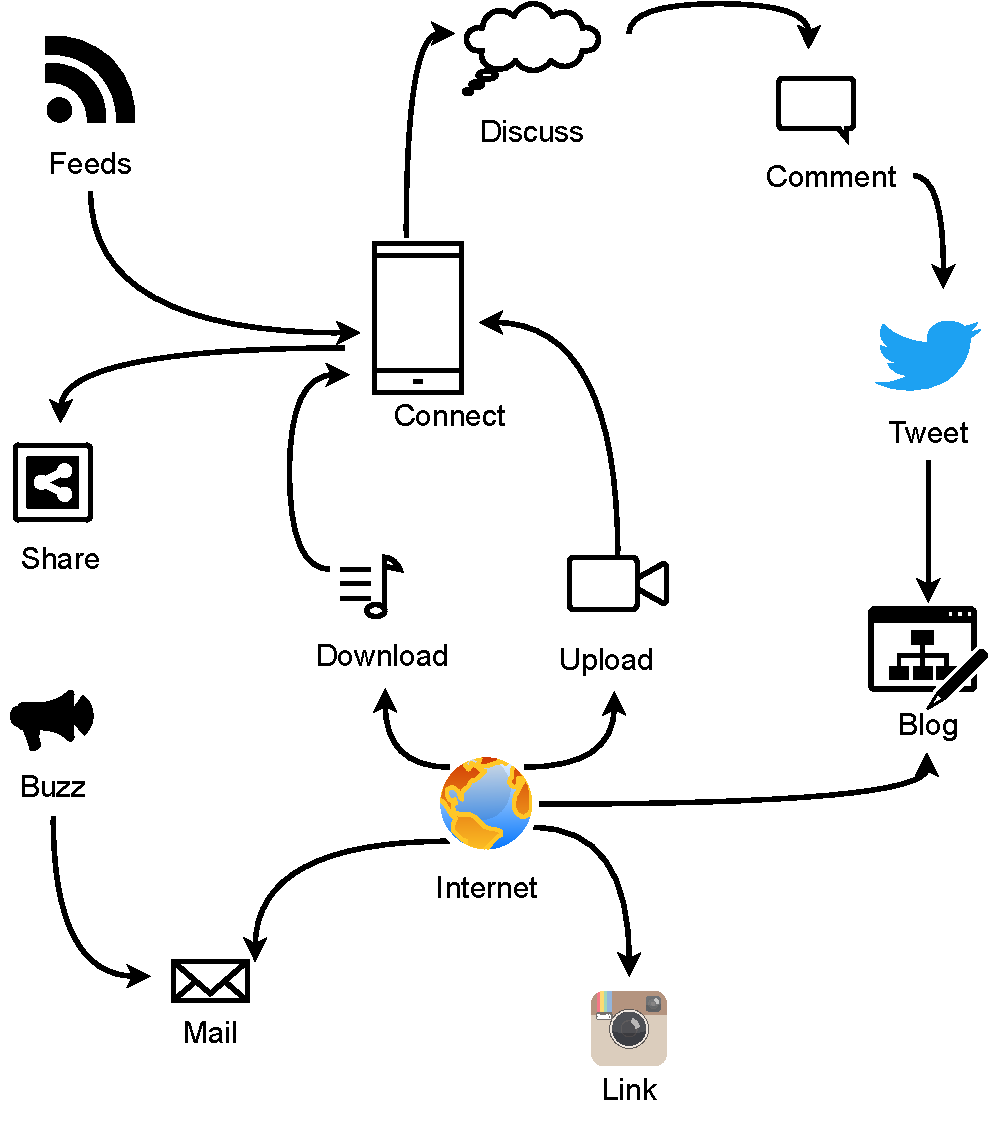
\includegraphics[width=0.4\textwidth]{figures/concepts/Web.pdf}
    \caption{Interactions on the Internet.}
    \label{fig:web}
\end{figure}

Data analysis for extracting information may be defiant. Such a task is even more complex if the analysis should take place in real-time. Under such a scenario, traditional processing systems based on the \textit{Batch processing} paradigm like \textit{MapReduce} \citep{DeanG08, CasadoY15} are not suitable for carrying out the analysis. Figure \ref{fig:batch-processing} shows a data pipeline using \textit{Batch processing}, where events are read to be processed periodically according to a time window, and, therefore, report are not generated online.

\begin{figure}[!ht]
    \centering
    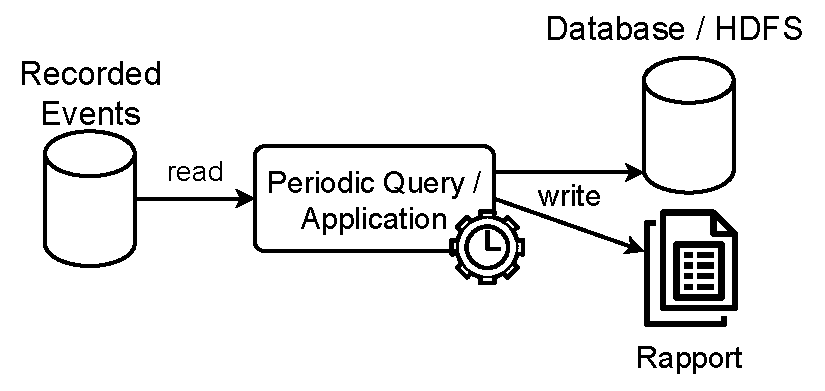
\includegraphics[width=0.7\textwidth]{figures/concepts/BatchProcessing.pdf}
    \caption{Batch processing concept.}
    \label{fig:batch-processing}
\end{figure}

Sustained on the need to process interactions in an online manner, different processing systems have been proposed in the literature. These systems are capable of dealing with unbounded sequences of events and deliver low-latency data. Nowadays, most users require quick and updated information online as a support for decision-making \citep{OzalRT11}.

A good example is social network analysis under post-disaster scenarios, where events are continuously generated, processing them as close to real-time as possible is necessary to obtain timely information to mitigate the disaster effects \citep{WladdimiroICTDM2016}. With such information, areas may be prioritized, resource distribution can be improved,  people searches may be more efficient, among others.

Another application is stock exchange prediction \cite{DingWPXL17}. In this case,  processing systems may analyze data and create mathematical models to predict the next day’s market behavior. 

In network security scenarios it is possible to monitor the network activity \citep{Zhao8230279}. As the data is processed in real-time, it may help to detect 'on the fly' malicious behaviors. A similar approach is followed on logs analysis. Online data processing makes it possible to detect bugs or errors, as well as to see if there is any intruder or system policy violation.

Stream Processing Systems (SPS) were specially designed to fulfill these needs \cite{Leibiusky0030281}. The goal of a SPS is to process unbounded continuous flows of events and to provide a scalable and efficient tool to process data close to real-time. Figure \ref{fig:stream-processing-concept} presents an example of a stream processing pipeline. Events are processed on the fly and aggregated results are stored in a database or presented on a dashboard.

\begin{figure}[!ht]
    \centering
    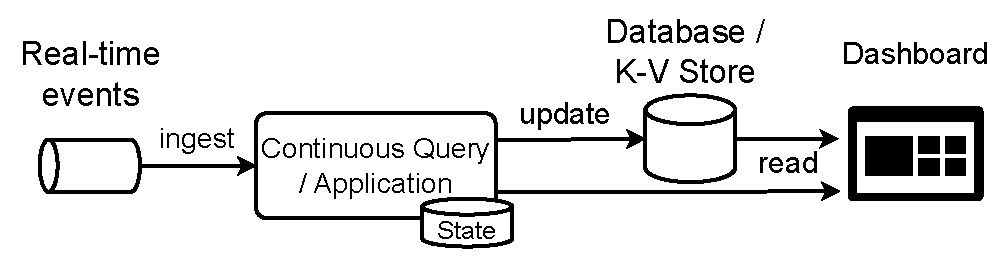
\includegraphics[width=0.95\textwidth]{figures/concepts/StreamProcessing-Concept.pdf}
    \caption{Stream processing concept.}
    \label{fig:stream-processing-concept}
\end{figure}

SPSs are based on directed acyclic graphs (DAG) whose vertices and unidirectional edges correspond to operators and event data flows respectively \cite{ChakravarthyJ09}. An external source continuously provides the data that the system consumes. Light programming tasks (like filters, counters, storage, etc.) are handled by operators that quickly and in pipeline-style process the data (events). In a processing infrastructure (e.g. clusters, clouds, etc.), resources (e.g., VMs) are allocated to execute the operators which are frequently replicated for performance reasons. Figure \ref{fig:sps-introduction} shows an example of a SPS application, whose pipeline is composed of one input data and four operators. In this example, each operator processes the events according to the pipeline flow, provided by the input data.

\begin{figure}[!ht]
    \centering
    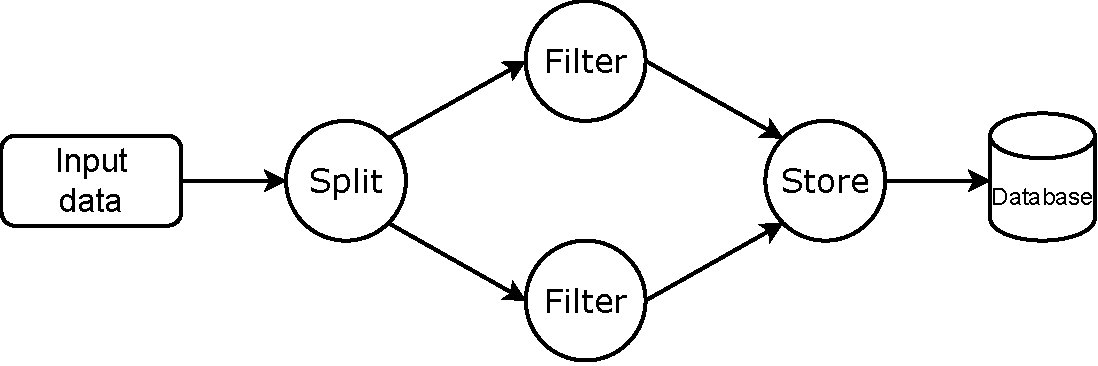
\includegraphics[width=0.95\textwidth]{figures/concepts/SPS-Introduction.pdf}
    \caption{Example of a SPS application.}
    \label{fig:sps-introduction}
\end{figure}

SPS frameworks, such as Storm \citep{Leibiusky0030281} or Flink \citep{CarboneKEMHT15}, are configured before their deployment, usually defining both the DAG and the number of operator replicas beforehand. There are works that adapt the number of replicas dynamically based on analysis of input fluctuation \citep{CardelliniPNR18, arkian2021model, KombiLLRB19}. However, replica reconfiguration usually requires stopping the application and restating it. For adapting the number of replicas, there exist basically two approaches. The reactive approach considers the state of the system, while the predictive analyses the history of the states.

Another critical feature of SPSs is the grouping strategy which is responsible for sharing the input load among operators' replicas. For instance, the round-robin policy is one of the most common approaches to implementing shuffle grouping.  However, the latter does not consider the input load of each replica, i.e., current queued events waiting to be processed.

The behaviour of data streams can be quite dynamic. Traffic behaviour may suddenly increase/decrease, and event distributions may be unbalanced, among others.  Such a dynamics may create struggle operators, increasing end-to-end latency and message loss. To solve this problem it is necessary to dynamically adapt the processing logic of the SPS, thereby increasing or decreasing the number of replicas of an operator, so a good adaptation decision may minimize the aforementioned problem: the latency and message loss can be reduced reaching higher accuracy for the data analysed.

For this reason, one solution is to propose an adaptive SPS, which characterize system utilization requirements and automatically increase/decrease the number of replicas of critical operators to keep latency restrictions and reduce event loss.

\section{Contributions}
\label{contributions}

%% 1. INTRODUCTION
This thesis proposes two adaptive SPSs (\rSPS{} and \pSPS{}) based on Storm \citep{toshniwal2014storm}. Its aim is to adapt the number of replicas of the operators according to the sparks in the data stream.
%% 2. MAPE Approach
Both adaptive SPS use the MAPE model \citep{ibm2005architectural}, which consists of a control loop composed of four modules: Monitoring, Analysis, Planning, and Execution.

%% 3. RA-SPS + PA-SPS
\rSPS{} and \pSPS{} exploit a reactive and predictive approach respectively. \rSPS{} bases its decision on the state of an operator at runtime, according to the analysis of traffic peaks in short periods of time.  \pSPS{} bases its decision on the behaviour of the input data and the number of operator active replicas required for processing the input data, finding patterns in the traffic to anticipate possible overloads, or underloads in the SPS.

%% 4. POOL
In order to cope with stream fluctuation both SPS, use a pool of operator replica, created beforehand. These replicas may be either active or inactive. Active replicas are deployed by the Storm scheduler. On the other hand, inactive replicas are idle, so they do not consume CPU resources but can be allocated as needed. Consequently, \textit{a pool of replicas} can be dynamically activated (resp., deactivated) when the system detects the need for increasing (resp., decreasing) the number of active replicas of an operator. Note that under this model, the stream processing systems can adapt without stopping the SPS.

%% 5. GROUPING
Another feature introduced in the proposed SPSs is the load-aware grouping that partitions the stream among replicas based on their respective current load.

%% 6. RA-SPS
\rSPS{} dynamically modify the number of replicas per operator based on a multi-metric. The multi-metric is composed of system statistics such as the queue size, the average execution time of an event, and the utilisation rate of an operator. It determines the state of the operators during a time interval, and depending on the state of the operator and conditions of the SPS, it is decided whether or not to modify the number of replicas.

%% 7. PA-SPS
\pSPS{} dynamically allocates the number of replicas per operator necessary to process the input stream, defining the events that each operator $O$ should process within a time interval. In order to predict the input stream and analyse the system's potential future behaviour, a predictive model is proposed, integrated to \pSPS{}. By considering both (1) the events sent to an $O$ by its direct operator predecessors as well as those from earlier time intervals that $O$ could not process at the time,  therefore, kept in a queue and (2) event execution time, the ideal number of $O$'s replicas for processing these events at each interval is deduced. As a result, the number of $O$'s replicas changes over time, depending on the input rate.

%% 8. EXPERIMENTS
This proposal is evaluated over the infrastructure of a well-known cloud provider, the Google Cloud Platform (GCP).  Performance was an exhaustive evaluation in terms of classical metrics such as end-to-end latency, resource utilization, the number of processed events, and the error of our estimations. This work presents, analyses, and discusses the results also comparing them with state of the art solutions. 

\section{Publications}
\label{publications}

Two articles in international conferences, two articles in French conferences, and one journal article submission under review. Chapter \ref{solution} presents the contributions of each article.

\subsection{International Conferences}
\begin{itemize}
	\item \cite{WladdimiroNCA} Daniel Wladdimiro, Luciana Arantes, Pierre Sens and Nicolas Hidalgo. "A Multi-Metric Adaptive Stream Processing System." In: \textit{NCA}. IEEE, 2021.
	\item \cite{WladdimiroSBAC} Daniel Wladdimiro, Luciana Arantes, Pierre Sens and Nicolas Hidalgo. "A predictive approach for dynamic replication of operators in distributed stream processing systems" In: \textit{SBAC}. IEEE, 2022.
\end{itemize}

\subsection{Journal}
\begin{itemize}
	\item \cite{WladdimiroJPDC} Daniel Wladdimiro, Luciana Arantes, Pierre Sens and Nicolas Hidalgo. "PA-SPS: A Predictive Adaptive Approach for an Elastic Stream Processing System" In: \textit{JPDC}. 2023. \textit{\textbf{[Under Review]}}
\end{itemize}

\subsection{National Conferences}
\begin{itemize}
	\item \cite{WladdimiroComPAS2022} Daniel Wladdimiro, Luciana Arantes, Pierre Sens and Nicolas Hidalgo. "A predictive model for Stream Processing System that dynamically calibrates the number of operator replicas." In: \textit{ComPAS}. Amiens, France, 2022.
	\item \cite{WladdimiroComPAS2023} Daniel Wladdimiro, Luciana Arantes, Pierre Sens and Nicolas Hidalgo. "PRESPS: a PREdictive model to determine the number of replicas of the operators in Stream Processing Systems" In: \textit{ComPAS}. Annecy, France, 2023.
\end{itemize}

\section{Organization}

The remaining of this theses is organised as follows:

%Chapter \ref{intro} was an introduction to the problem of real-time data processing, as well as an explanation of the adaptability problem in a SPS.

Chapter \ref{background} gives the necessary concepts for the understanding of SPSs, the architecture of the SPS frameworks, and our contribution.

Chapter \ref{related-work} presents related work about adaptive SPS. Existing solutions use a manual approach, which depends on a user for modifying the SPS, or a automatic approach, where the SPS is in charge of the adaptation.

Chapter \ref{solution} presents the proposed SPSs(\rSPS{} and \pSPS{}) as well as the pool of replicas and \textit{Load-Aware} grouping approach.

Chapter \ref{experimentation} presents evaluation results related to \rSPS{} and \pSPS{} experiments conducted on GCP.

Finally, Chapter \ref{conclusion} presents the conclusion and some future work.
% !TEX root = ../main.tex
%
\chapter{Background}
\label{background}
This section introduces some concepts used in this work. First, we define what is stream processing. This is important since it characterizes the behaviour of events collected from data sources under this paradigm. Then, we introduce the Stream Processing Systems (SPS), both the system and its components, and some frameworks used to implement them.


\section{Stream processing}
\label{stream-processing}
%\section{Streaming}
Streaming refers to a continuous flow of data that is generated, transmitted, and processed in real time over a network \cite{Menin2002SMH}. It allows users to access and consume its content as it is under transmission, so there is no need to store all the content before using it. It consists of an external entity sending data to a data processing system. If the service is busy, the data is queued. Generally, streaming is used by web interaction, such as social networking or online playback of multimedia content.

Streaming is largely used in processing information in real-time, when the temporality of the data is relevant, such as online playback of multimedia material. For instance, Streaming API provided by Twitter, can be used to study the most relevant tweets, trending topics or hashtags for specific cases such as election campaigns or natural disasters. Streaming is processed by SPSs.

\begin{figure}[ht!]
  \centering
    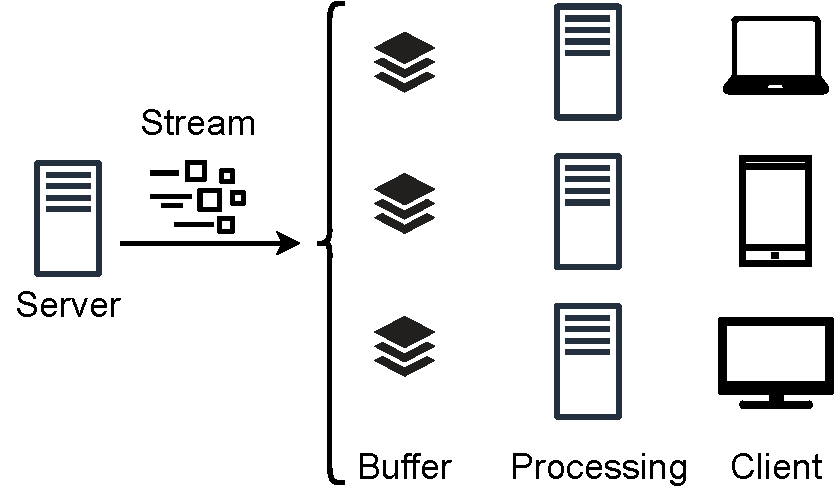
\includegraphics[scale=0.6]{figures/concepts/Streaming.pdf}
  \caption{Streaming example among server and clients.}
  \label{fig:streaming}
\end{figure}

Figure \ref{fig:streaming} shows a server emitting a data stream, which is received by different clients. Each client is in charge of processing the received data, if the client is busy, data is buffered. Otherwise the client will process the data according to the service policy.

%\section{Stream processing}

Stream processing is a computing paradigm and data processing approach that involves the continuous processing of data as it is generated and ingested in real-time. This paradigm focuses on programming applications that can process information on the fly as close to real-time as possible, using system resources in a parallel or distributed manner to meet their objective. It is typically used for real-time applications that close to real time responses, such as monitoring, fraud detection, and predictive maintenance.

Figure \ref{fig:stream-processing} presents a Stream processing scenario. The input stream corresponds to the input stream of external data, which is delivered by an external source such as sensors, log records, or database transactions. Each data is a basic unit, which is processed to obtain relevant information. The stream process is the component in charge of processing the input stream.
These processes can be stateful, so if necessary, the processing status is stored in an external database. It is also possible to process several data in parallel, either using more logical or physical resources. The output stream is the processed data, which can be used as a data stream to be processed or stored.

\begin{figure}[ht!]
  \centering
    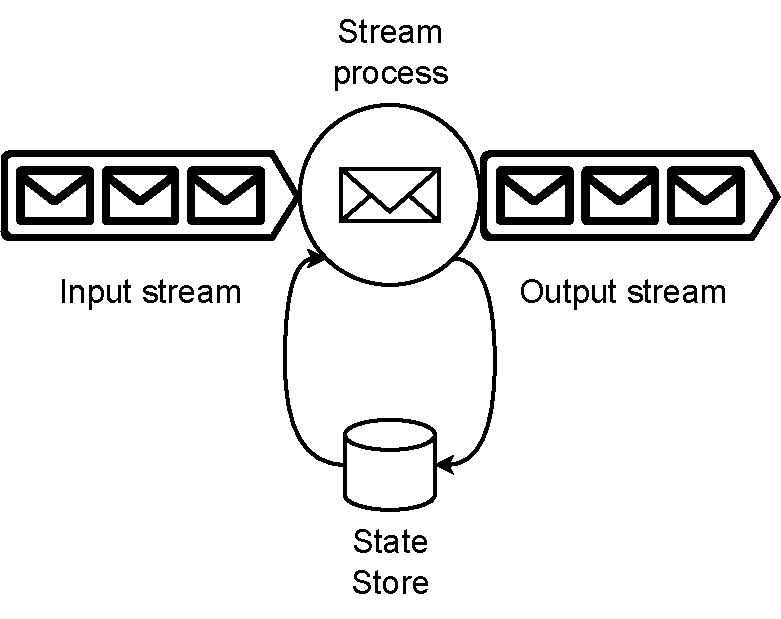
\includegraphics[scale=0.6]{figures/concepts/StreamProcessing.pdf}
  \caption{Stream processing paradigm.}
  \label{fig:stream-processing}
\end{figure}

For the correct functioning of these applications, some requirements should be satisfied. The work \cite{andrade2014fundamentals} defines them, which are classified as follows:

\begin{itemize}
	\item \textbf{Processing large quantities of distributed data}: One of the main goals of Stream processing is the processing of large volumes of data, which are sent in a distributed manner by external sources. By processing these data, the system can monitor, analyse, or control them in real-time, since the data processing is performed as the data stream continues.
	\item \textbf{Addressing stringent latency and bandwidth constraints}: This point refers to a stable connection between components over the network, where bandwidth or latency is not a limiting factor for data processing. Such a requirement is important since an application that considers data in real time is useless if it presents a high latency. Low latency should always be maintained, so that the data is as close to real time as possible.
	\item \textbf{Processing heterogeneous data}: A standard both in the data structure and its format should be application in the raw data from external sources that are used in the Stream processing. In this way, the processing will be homogeneous for all data, avoiding problems associated with the data structure.
	\item \textbf{Providing long-term high availability}: SPS operators can fail which inducing the decrease of data throughput. Thus, it is important to have a fault tolerance mechanism to reduce the loss of information. In the order, provide a constant processing of data, which is stable and persistent over time. Otherwise, information can be lost, compromising the accuracy of the results and requiring more time to collect the lost information or reach a similar state.
\end{itemize}

\section{Stream Processing Systems}
A Stream Processing System (SPS) is a software or framework designed to process and analyze data streams in real-time, which is based on the concepts of Stream processing. The main goal of an SPS is to process high volumes of data in a distributed way and in real-time \cite{kleppmann2016making}. In contrast to the traditional batch processing model, which stores the data to later process it offline \cite{HawwashN14}. SPS shift involves the analysis of data without requiring storage.

The paradigm used by SPSs is based on a directed acyclic graph (DAG) as shown in Figure \ref{fig:sps-concept}. The operators correspond to the vertices of the graph, such as analyzers, word filters or some particular algorithm, while the edges correspond to the dataflow between operators \cite{Shahrivari14}. In addition, the input data (the source) is originated by an external entity, such as streaming from social networks, statistics from the monitoring of a system, or transactions in the stock exchange. The first operator consumes data from the source \cite{AppelFFB12}. In most graphs, the terminal operators are in charge of storing the results of the data processing in a database.

\begin{figure}[ht!]
  \centering
    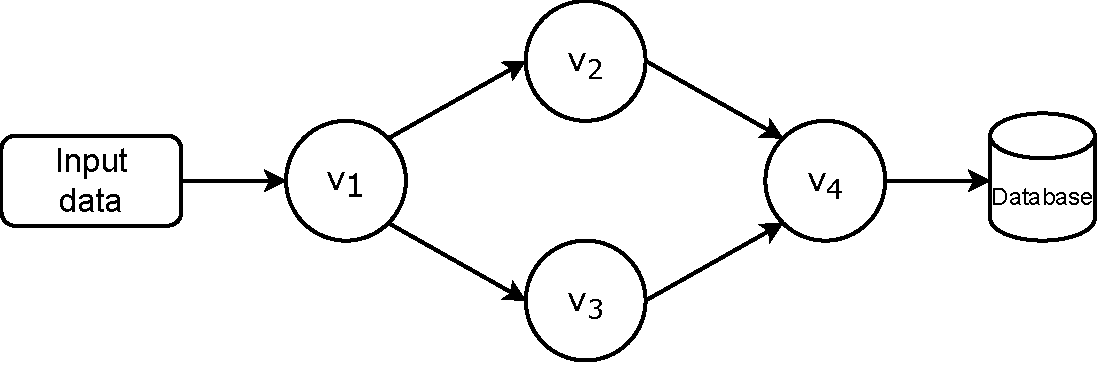
\includegraphics[scale=0.6]{figures/concepts/SPS-Concept.pdf}
  \caption{Example of the representation of the DAG in an SPS application.}
  \label{fig:sps-concept}
\end{figure}

It should be noted that SPSs are distributed, i.e., each vertex is hosted in a physical node available in the environment where the system is hosted, either a \textit{cluster}, a \textit{grid} or a \textit{cloud}. To achieve communication between the operators, systems specially designed for this type of task are used, such as Apache ZooKeeper \cite{HuntKJR10}. The latter consists of a centralized orchestration that maintains configuration and synchronization information of the distributed applications. To this end, each processing node must register in the system, and it is the orchestrator that is subsequently in charge of synchronizing the nodes available for processing and distributing the events among them.

Most applications running on SPS, manage large amount of data, which must be processed to obtain information or statistics, as , for instance, fraud detection, collection of information in case of disasters or analysis of interaction in social networks. To perform real-time processing of the data, \cite{StonebrakerCZ05} establishes the following requirements:

\begin{itemize}
		\item \textbf{Keep the Data Moving}: To ensure low latency in the processing of high volumes of data, it is necessary to preclude the storage of the data when processing it, since the storing data adds unnecessary latency to the system. Thus, the aim is to process data "in-stream", i.e., as the data is received, it is processed.
        \item \textbf{Query using SQL on Streams}: To reduce the development and programming time of projects, it is important to provide an abstraction in the operations performed by the program, as done by a high-level language such as SQL. In this way, there is a set of default functions, which we can be use to query, group, join, or modify, accepted by most popular DBMS. Thus, providing a support to  StreamSQL, a variant of SQL designed for SPS, ends up being an important tool for the SPS ecosystem.
        \item \textbf{Handle Stream Imperfections}: Because data are processed in-stream, it is necessary to provide a provision model for handling data that is delayed, missing, or out-of-order. Hence, if the SPS is performing an operation that considers a calculation in a time window, a mechanism must be provided to handle delayed or out-of-order events. On the other hand, if the system is waiting for a missing data, which might never arrive, then a timeout mechanism should avoid that the system blocks forever.		        
        \item \textbf{Generate Predictable Outcomes}: SPS can predictably process data, always given the same results. This means that the process must be deterministic and repeatable. Such a behaviour reflects the fault tolerance provided by the SPS, given that in the case of data loss, data recovery is possible and the result remains the same.
		\item \textbf{Integrate Stored and Streaming Data}: Some applications may be composed of stateful operations. For instance, the word-counting operator requires variables that store the statistics of the incoming stream. Therefore, the SPS must provide a system for storing, accessing and modifying the states used by the application. These states can also be added to the data in the stream, so it is important to
have a uniform language to deal with both components.
        \item \textbf{Guarantee data security and availability}: SPS must provide data fault tolerance mechanism to ensure data integrity and provide integrity to the processing of critical data information. In this way, the system must provide checkpoint management for both data integrity and state. Thus, in case of data processing failure, the system will be able to reprocess data. 
		\item \textbf{Partition and Scale Applications Automatically}: The distribution of an SPS is important both in terms of scalability and cost. By using the system on a single machine, resource constraints are likely to happen. Likewise, the costs associated with distributing a system across multiple machines are higher. Therefore, the SPS should ideally provide a transparent and automatic distribution of operators on the available machines, providing scalability in its processing.
       \item \textbf{Process and Respond Instantaneously}: When considering the use of SPS, a system is required to respond close to real-time. Therefore, the SPS must provide a solution that copes with operator overloads, which affect system performance. The solution should present low overhead, i.e., small implementation cost or resources requirements, increasing, thus, the efficiency and performance of the system.
\end{itemize}

\subsection{Stream}

Stream is a continuous flow of data records or events that are processed and analysed in real-time. It represents a sequence of data elements that arrive continuously over time. Stream is the fundamental building blocks in SPS corresponding to the input and output channels for data processing. They can represent various types of data, such as sensor readings, log entries, financial transactions, social media updates, or any other type of event-based data.

Streams in SPS typically exhibit the following characteristics \citep{SilvaFBHCG13}:

\begin{itemize}
\item \textbf{Continuous flow}: Streams are continuous and persistent, with data flowing continuously over time. Data arrived are generated, transmitted, and added to stream, creating a dynamic traffic.

\item \textbf{High data arrival rate}: In Streams usually data arrives at a high rate or frequency, requiring SPSs to handle and process data in real-time or near real-time to keep up with the incoming data.

\item \textbf{Potentially unbounded}: Streams can be unbounded, meaning that there is no predefined endpoint or limit. They can continue indefinitely, and the processing system needs to handle the continuous arrival of data without assuming an end.

\item \textbf{Ordered or unordered}: Streams can be ordered, where the order of events is meaningful and needs to be preserved during processing. On the other hand, if the order of events is not important, processing can occur independently on each event.

\item \textbf{Potentially partitioned}: In distributed stream processing systems, streams can be partitioned into multiple partitions or shards. Each partition contains a subset of the data, and, thus, for parallel processing across multiple nodes or processing units can take place.
\end{itemize}

Streams are the primary input to SPS, and then they are ingested, processed, and transformed by various operators or computations. The processed results or derived streams can also be emitted as outputs for further processing, storage, visualization, or integration in other systems.


\subsection{DAG}
A directed acyclic graph (DAG) defines the processing logic of the SPS where each vertex represents an operator, and unidirectional edges (arcs) represent the dataflow. The DAG is defined as $G=(V,A)$, where $V$ is the set of vertices and $A$ is the arcs group. Likewise, $n$ represents the number of vertices in $V$ and $m$ represents the number of arcs in $A$. Each vertex corresponds to an operator, and each arc corresponds to a stream in the SPS application. For example, Figure \ref{fig:sps-dag} shows a DAG, where $G=(V,A)$ with $V=\{\text{v}_1,\text{v}_2,\text{v}_3,\text{v}_4\}$ and $A=\{\text{a}_1,\text{a}_2,\text{a}_3,\text{a}_4,\text{a}_5\}$, $n=4$ and $m=5$. In this case, the initial vertex is $\text{v}_1$ and the terminal vertex is $\text{v}_4$.

\begin{figure}[ht!]
  \centering
    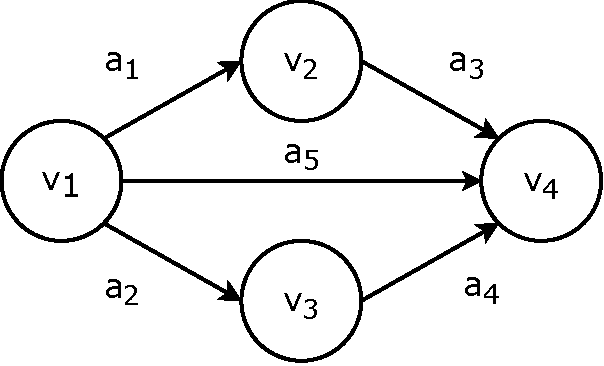
\includegraphics[scale=0.6]{figures/concepts/SPS-DAG.pdf}
  \caption{DAG in an SPS.}
  \label{fig:sps-dag}
\end{figure}

A path $v$ is a sequence of vertices and arcs defined as $v=\text{v}_i\text{a}_k\text{v}_j...\text{v}_p\text{a}_l\text{v}_{q}$, where $\text{v}_i, \text{v}_j, \text{v}_n, \text{v}_m \in V$ for $i,j,p,q \in \{1,...,n\}$ and $\text{a}_k=\{\text{v}_i,\text{v}_j\}, \text{a}_l=\{\text{v}_p,\text{v}_q\} \in A$. Therefore, since in DAGs there are no cycles, the first and last vertices in the path are not the same, i.e., $\text{v}_i \neq \text{v}_q$. For example, in the Figure \ref{fig:sps-dag} it is possible to trace a path between $\text{v}_1$ and $\text{v}_4$, defined by $v_1=\text{v}_1a_1\text{v}_2a_3\text{v}_4$, $v_2=\text{v}_1a_2\text{v}_3a_4\text{v}_4$ or $v_3=\text{v}_1a_5\text{v}_4$, without having cycles.

For a DAG $G=(V,A)$, it is possible to associate the relation $\le$ defined by: for any pair of vertices $(\text{v}_i,\text{v}_j) \in v$ for $i, j \in \{1,...,n\}$ , $\text{v}_i \le \text{v}_j$ if there exists a path $v$ from $\text{v}_i$ to $\text{v}_j$ in $G$. In this way, a topological ordering of $G$ is defined as a list $(\text{v}_i,...,\text{v}_j)$ of vertices of $G$ for $i,j \in \{1,...,n\}$, such that if $i \le j$, then there is no path between $\text{v}_j$ to $\text{v}_i$. For example, Figure \ref{fig:sps-dag} has the list $(1,2,3,4)$ or $(1,3,2,4)$. The ordering is unique, only in the case that a path connects all the vertices, and corresponds to the order in which the vertices appear.

Paths can start from different vertices. Thus, depending on its origin, the set of vertices of different paths is not the same. Figure \ref{fig:sps-dag-complex} presents a complex DAG, where there are two initial vertices ($\text{v}_1$ and $\text{v}_5$) and two terminal vertices ($\text{v}_4$ and $\text{v}_7$). In the case of choosing $\text{v}_1$ as the initial vertex, it is possible to end at $\text{v}_4$ or $\text{v}_7$, but not in the case of $\text{v}_5$, since it can only end at $\text{v}_7$. By taking different paths, the application relies on different operators, so processed data also varies.

\begin{figure}[ht!]
  \centering
    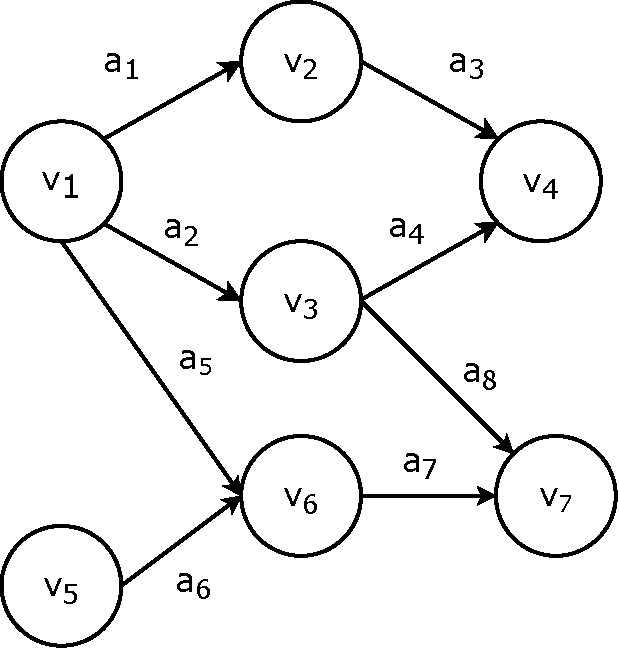
\includegraphics[scale=0.6]{figures/concepts/SPS-DAG-Complex.pdf}
  \caption{DAG complex in an SPS.}
  \label{fig:sps-dag-complex}
\end{figure}

\subsection{Tuples}
The SPS must process structured input data. Therefore, initial operators are used to structure the input data, which can be structured, semi-structured or unstructured. Thus, each structured data created by an external data source is called tuple. A tuple is a basic unit of data that is defined by \textit{(key, value)}, a set of attributes or fields, which flow through the application graph. Each tuple is a single event in the data stream, which is often used to represent an event such as sensor reading, user action, or a financial transaction in real-time applications such as monitoring, alerting, or fraud detection. In general, a tuple has the timestamp of its creation, as well as the timestamp of its predecessor vertices in the DAG. The number and type of attributes in a tuple depend on the need of the application, as well as the path taken by the tuple.

\begin{figure}[ht!]
  \centering
    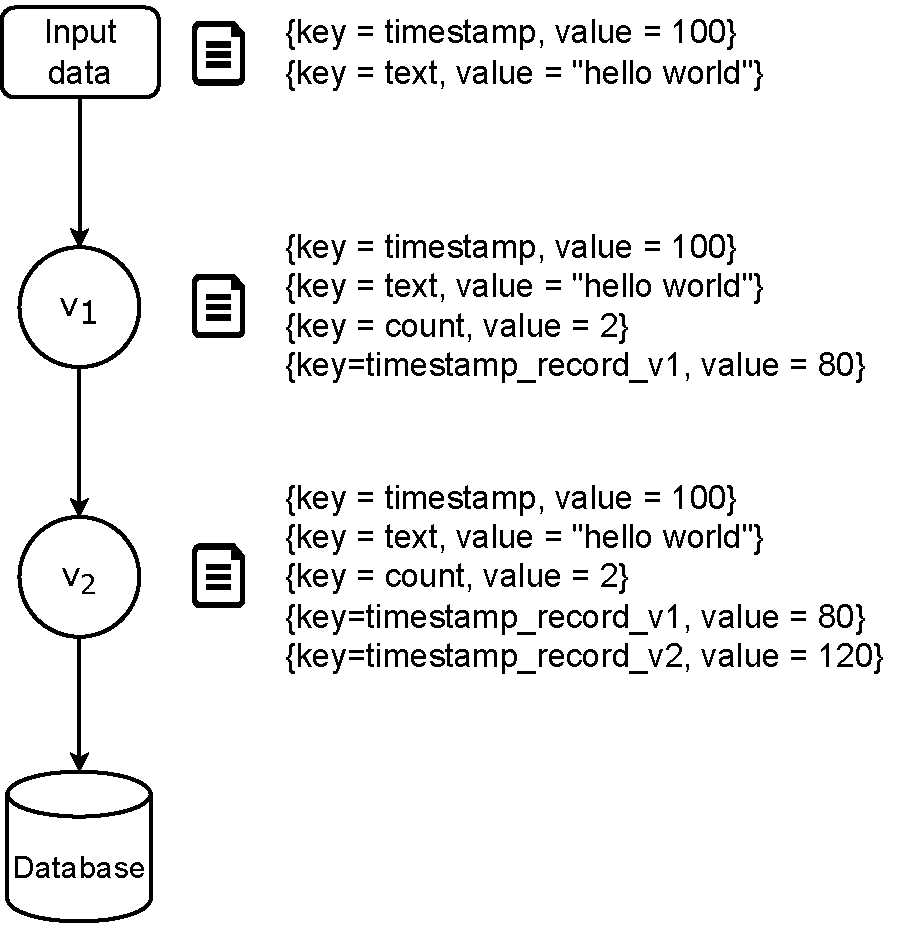
\includegraphics[scale=0.6]{figures/concepts/SPS-Tuple.pdf}
  \caption{The tuple exchange in an SPS.}
  \label{fig:sps-tuple}
\end{figure}

Figure \ref{fig:sps-tuple} presents the flow of a tuple through SPS application, which is defined by four components: input data, two operators and a database. Operator $\text{v}_1$ counts the number of words in the stream, and operator $\text{v}_2$ stores the tuples in a database. The start of the flow begins with the input data, structured in key-value. After this, the tuple is sent to operator $\text{v}_1$, which determines that the number of words is 2. Therefore, it adds a new field \texttt{count} to the tuple and the timestamp record, and sends it to operator $\text{v}_2$. Finally, the $\text{v}_2$ operator stores the tuple in a database, adding the timestamp record.


\subsection{Operator}
An operator is a processing unit that receives data from one or more input streams, performs some computation on the data, and produces one or more output streams. An operator is represented by a vertex in the DAG. The majority of operators are designed to perform light tasks, nevertheless, they can also implement complex tasks, depending on the design of the SPS application.

Depending on the DAG, operators can be replicated and the income data is processed in parallel. Also, each operator has a level of parallelism, which is related to the SPS implementation. Same solutions propose to associate parallel unit to logical resources (i.e. processes or thread), and others to physical resources (i.e. containers or VM).

Figure \ref{fig:sps-operator-parallelism-dag} shows the DAG for an SPS application. The DAG is composed of three operators: $\text{v}_1$, $\text{v}_2$ and $\text{v}_3$. Due to the complexity of operator $\text{v}_2$, the application requires increasing the parallelism of the operator. Figure \ref{fig:sps-operator-parallelism-logical} shows the parallelization of the operator $\text{v}_2$, where $k$ replicas of the operator are created to process data in parallel.

\begin{figure}[!ht]
\begin{center}
\subfloat[Representation by DAG.]{
  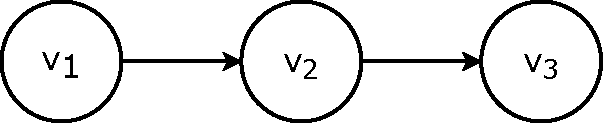
\includegraphics[scale=0.55]{figures/concepts/SPS-Operator-Parallelism-DAG.pdf}
  \label{fig:sps-operator-parallelism-dag}
}

\vspace*{0.5cm}

\subfloat[Representation of operator parallelisation.]{
	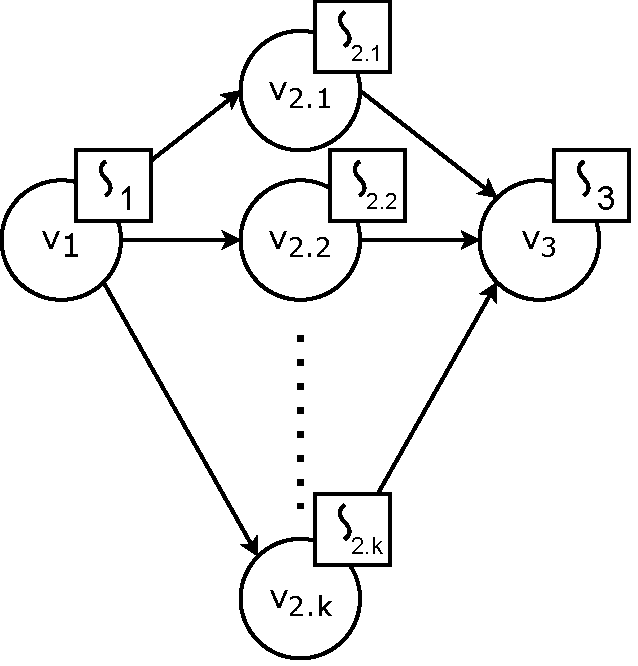
\includegraphics[scale=0.55]{figures/concepts/SPS-Operator-Parallelism-Logical.pdf}
    \label{fig:sps-operator-parallelism-logical}
}
\caption{Example of parallelism of an SPS operator.}
\label{fig:sps-operator-parallelism}
\end{center}
\end{figure}

Data is represented by tuples, so operators process tuples. Depending on the operator's task, tuples are sent without or with modification. It is also possible to discard them, create new tuples, or on the other hand, to perform some analysis on them. Futhermore, depending on whether or not the operator maintains the state or context of the data it processes, operators are classified into: \textit{stateless} and \textit{stateful}.

Stateless operators do not maintain the internal state or context of the data. They are independent tasks that depend only on the input tuples, without the need to know the past processing or global state of the application. These types of operators are used to perform operator-specific tasks. Stateless operators are associated with mapping, filtering, and data transformation tasks in the SPS.

\begin{figure}[ht!]
  \centering
    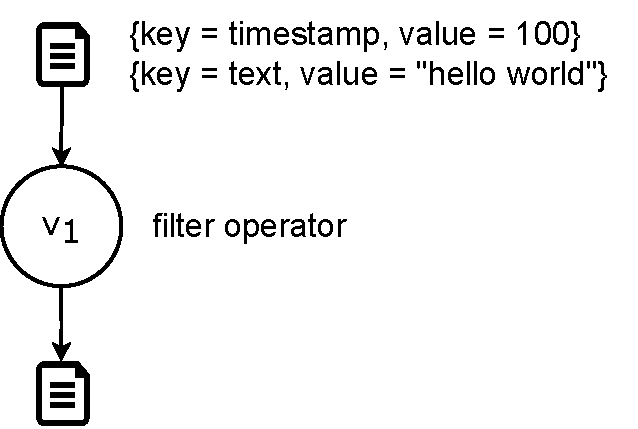
\includegraphics[scale=0.6]{figures/concepts/SPS-Stateless-Operator.pdf}
  \caption{An example of stateless operator.}
  \label{fig:sps-stateless-operator}
\end{figure}

Figure \ref{fig:sps-stateless-operator} presents an operator $\text{v}_1$ that performs a filtering task, which analyses if the text is in english written. If it is not, the event will not continue in the pipeline. In most cases, stateless operators are easily parallelizable, because it is not necessary to have consistency in the state of replicated operators, so they have a high scalability, which is useful for processing large amounts of data. When these operators are restarted, they have no impact in the overall processing of the data.

For stateful operators, the output depends on the internal state of the operator.  Therefore, they require past knowledge of the events or global state of the SPS to perform the task effectively. Such tasks are associated with windowed aggregations, pattern detection, or any operation that requires continuous analysis of data over some time.

\begin{figure}[ht!]
  \centering
   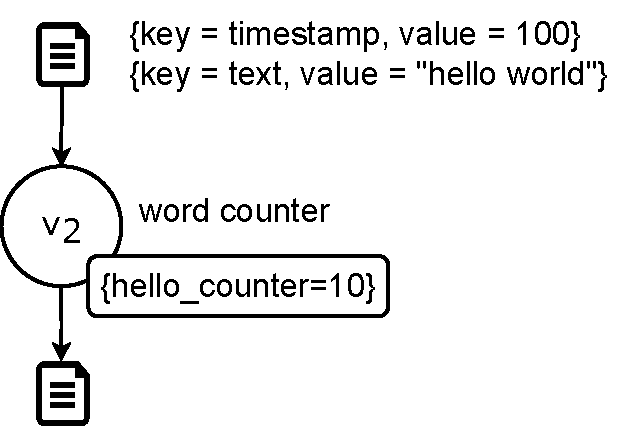
\includegraphics[scale=0.6]{figures/concepts/SPS-Stateful-Operator.pdf}
  \caption{An example of stateful operator.}
  \label{fig:sps-stateful-operator}
\end{figure}

Figure \ref{fig:sps-stateful-operator} presents operator $\text{v}_2$ which has a state that stores a counter indicating the number of tuples containing a specific word under a time window. Initially the operator $\text{v}_2$ has a state \texttt{hello\_counter=9}. Thus, after counting the incoming event the internal state will be \texttt{hello\_counter=10}. This state can be stored in memory or in an external database. The management of its state increases complexity, due to data consistency, fault tolerance, and scalability of the operator, because, as the number of replicas of this operator increases, it is necessary to ensure the consistency of the replica states.

\section{SPS Frameworks}
\label{sps-frameworks}
In this section, we will present two popular SPS frameworks: \textit{Storm} and \textit{Flink}. The logical architecture will be presented, with the components that make up the DAG, as well as the physical architecture, explaining the components necessary for its deployment and communication.

\subsection{Storm}

Storm \citep{toshniwal2014storm} is a distributed SPS framework implemented in Java and Clojure that enables the processing of unbounded streams of data. It was initially developed by the BackType team, which was later acquired by Twitter. It is an open-source Apache project, so there is a strong community of developers involved.

\subsubsection{Logical architecture}

A Storm application is represented by a DAG, also referred as \textit{Topology}. There are three types of components in a \textit{Topology}: \textit{Streams}, \textit{Spouts}, and \textit{Bolts}. 

\textit{Streams} are a sequence of tuples created and processed in parallel following the DAG model. These are distributed around the application. \textit{Streams} are composed of a structure of key-value tuples. Tuples can be defined by bytes, numbers, booleans or strings. Each \textit{Stream} must be declared by a unique identifier.

\textit{Spouts} are responsible for capturing the input data from external sources. They consume events and generate tuples sharing them to other \textit{Bolts} downstream in the \textit{Topology}. \textit{Spouts} can be implemented in either reliable or unreliable fashion. A reliable \textit{Spout} is capable of resending the same tuple in case it fails. Otherwise, it forgets to resend the tuple once it is emitted.

In \textit{Storm}, operators are called \textit{Bolts}. In general, these are lightweight tasks, so complex operations are designed as a pipeline of operators. \textit{Bolts} can receive the tuples emitted from one or more \textit{Streams}. Similarly to \textit{Spouts}, \textit{Bolts} can send the processed tuples through one or more \textit{Streams}. To guarantee processing, \textit{Bolts} can send an ACK (acknoledgement) message to indicate a tuple was processed. Each \textit{Bolt} is parallelizable, so it has an associated parallelism degree, which corresponds to the number of replicas of an operator.

\begin{figure}[!ht]
    \centering
    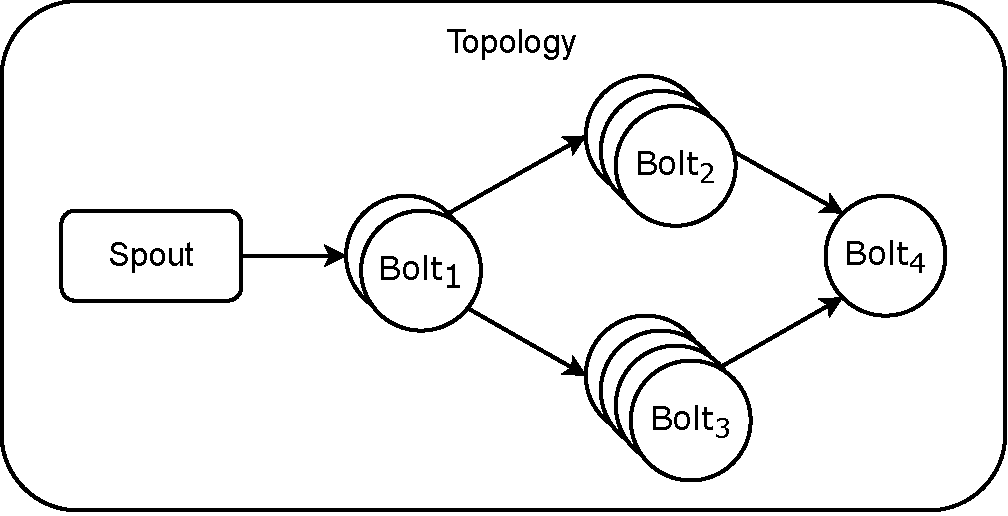
\includegraphics[width=0.75\textwidth]{figures/concepts/Storm-Logical.pdf}
    \caption{A Storm \textit{Topology} and components.}
    \label{fig:storm-logical}
\end{figure}


Figure \ref{fig:storm-logical} shows an Storm \textit{Topology} (DAG) example, composed of \textit{Spout}, and four \textit{Bolts}. The number of replicas for $Bolt_1$, $Bolt_2$, $Bolt_3$ and $Bolt_4$ are $2$, $3$, $4$ and $1$ respectively. $Spout$ is in charge of sending the raw data to $Bolt_1$ by distributing the stream data input to each of $Bolt_1$'s replicas based on some stream grouping. After processing the tuple, $Bolt_2$ sends the processed tuple to $Bolt_2$ and $Bolt_3$, the following \textit{Bolts} downstream in the DAG. If there is not \textit{Bolt} downstream, we are in presence of a sink operator and dataflow is terminated. The last operator that processes the data in \textit{Topology} is $Bolt_4$.


In the presence of \textit{Bolt's} replicas in Figure \ref{fig:storm-logical}, \textit{Stream} is partitioned and shared among them as shown in Figure \ref{fig:storm-stream-grouping}, which is defined by \textit{Stream grouping}. Every \textit{Bolt}'s replica processes the received tuple and sends the processed tuple to the next based on some stream grouping. Therefore, for each defined \textit{Stream} it is necessary to define \textit{Stream grouping} for sending a tuple between two components.

\begin{figure}[!ht]
    \centering
    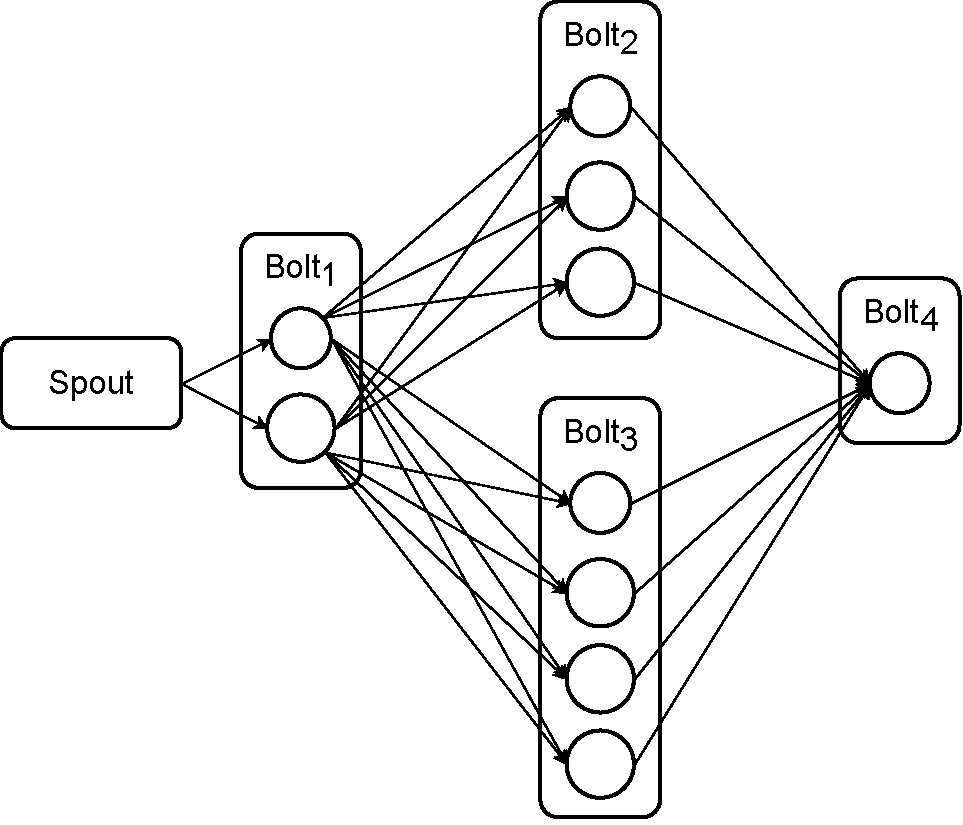
\includegraphics[width=0.75\textwidth]{figures/concepts/Storm-Stream-Grouping.pdf}
    \caption{Stream grouping in a Storm \textit{Topology}.}
    \label{fig:storm-stream-grouping}
\end{figure}

Storm has defined eight \textit{stream groupings}, can be used. If necessary, it is possible to define new \textit{stream groupings}.

\begin{enumerate}
\item \textit{Shuffle grouping}: Tuples are sent randomly to each replica.
\item \textit{Fields grouping}: The stream is partitioned by a field given in the tuple that determines which replica will receive the tuple.
\item \textit{Partial Key grouping}: This stream grouping is proposed by \cite{NasirMGKS15}. Similarly to \textit{Fields grouping}, it used a specific field for the choise of the replica, but also considers the load balancing between the available replicas.
\item \textit{All grouping}: Tuples are sent to all replicas.
\item \textit{Global grouping}: Tuples are sent to a single replica.
\item \textit{None grouping}: Tuples are sent randomly to each replica but in this case the same thread is always used by the assigned \textit{Bolts}.
\item \textit{Direct grouping}: Tuples are sent directly to the desired replica according to some attribute declared in \textit{Stream}.
\item \textit{Local grouping}: Tuples are sent to a group of replicas sharing the same resources.
\end{enumerate}

Except \textit{Partial Key grouping}, the drawback of these approaches is the potential lack of load balance. To cope with such a problem, other existing SPS propose hash-based data partition\citep{ShahHCF03}, partial-key based \citep{NasirMGKS15} or executor-centric solutions \citep{WangFMWZ19}.

Storm parallelism implementation is based on three concepts: \textit{Tasks}, \textit{Executors} and \textit{Worker processes}.

\textit{Tasks} are defined as data processing units, being replicas of a \textit{Bolt} or \textit{Spout}. While by default a task is assigned to one thread, it is possible to assign several tasks to the same thread.

An \textit{Executor} is a thread. One or more \textit{Tasks} of the same type (\textit{Bolt} or \textit{Spout}) can be assigned within the \textit{Executor}.

\textit{Worker processes} are a subset of a \textit{Topology}, so its in charge to run a set of \textit{Executors}. A \textit{Worker process} is a physical JVM. Each \textit{Worker process} is assigned to a machine and allocated resources can be configured according to the latter.

Figure \ref{fig:storm-parallelism} shows the parallelism of the Storm \textit{Topology} of Figure \ref{fig:storm-logical}. The \textit{Topology} has three subsets represented by \textit{Workers processes}, which are distributed on physical machines. Each \textit{Bolt} and \textit{Spout} represent a \textit{Task}, and each \textit{Task} is associated with a single \textit{Executor}, except in the case of $Bolt_2$, where all \textit{Tasks} are associated with a \textit{Executor}. In summary, the number of associated threads for each \textit{Bolt} is $Bolt_1 = 2$, $Bolt_2 = 1$, $Bolt_3 = 3$ and $Bolt_4 = 1$.

\begin{figure}[!ht]
    \centering
    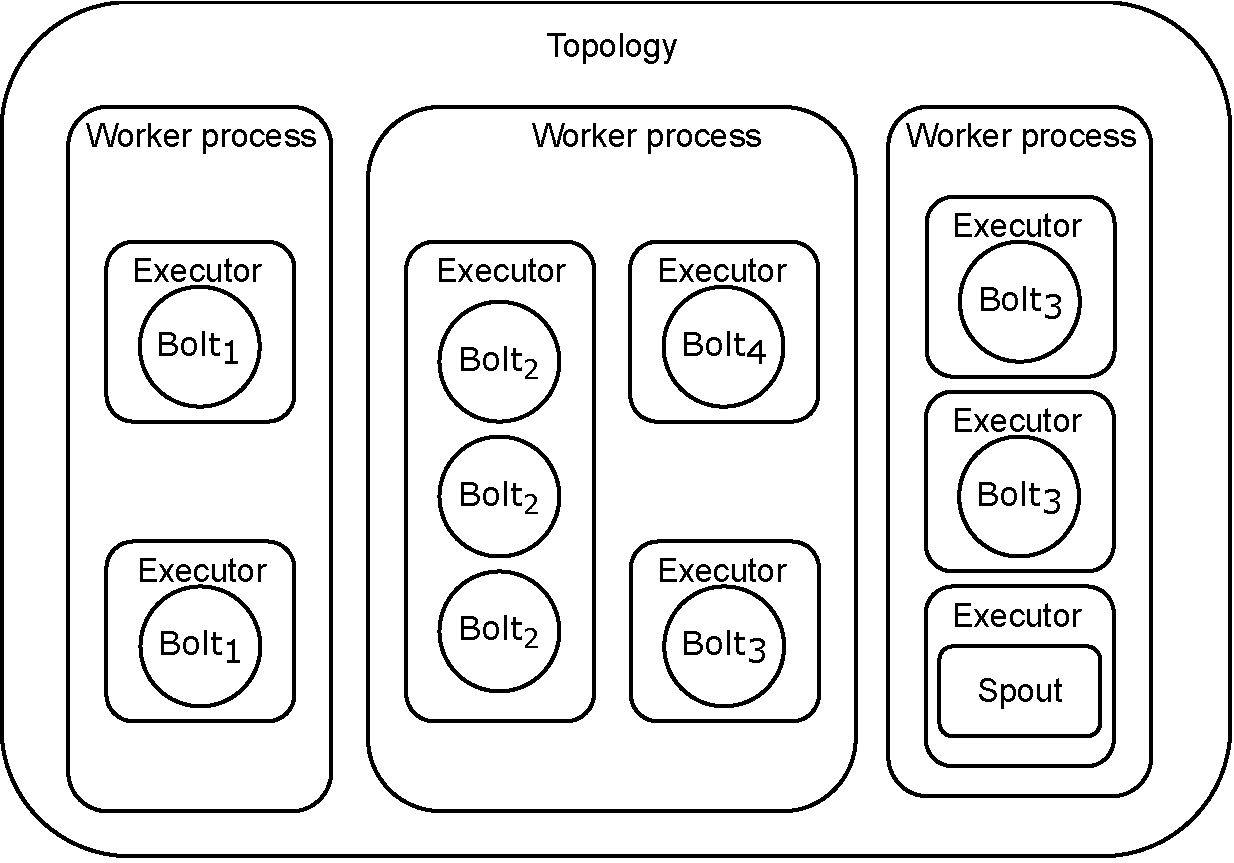
\includegraphics[width=0.75\textwidth]{figures/concepts/Storm-Logical-Parallelism.pdf}
    \caption{Parallelism of a Storm \textit{Topology}.}
    \label{fig:storm-parallelism}
\end{figure}

\subsubsection{Physical architecture}

Storm \textit{Topology} is deployed in a \textit{Storm Cluster}, which is a physical environment for its execution. Its components, hosted on machines, cores or VMs, are distributed on a platform such as a Grid, Cluster or Cloud. There are two kinds of components: \textit{Worker node} and  \textit{Master node}.

The \textit{Worker node} is responsible for hosting Storm \textit{Topology} tasks. Each \textit{Worker node} runs a daemon called \textit{Supervisor}. The role of the \textit{Supervisors} is to host one or more \textit{Worker processes}, so they deploy a subset of Storm \textit{Topology}. Thus, when deploying a Storm \textit{Topology} on a set of \textit{Worker processes}, each associated task will be distributed around \textit{Storm Cluster}.

The master node runs a daemon called \textit{Nimbus}, which is responsible for distributing the associated Storm \textit{Topology} code around the \textit{Storm Cluster}. At the same time, \textit{Nimbus} detects distributed component failures (i.e. node crashes or loss of messages) and the state of nodes. Finally, \textit{Nimbus} runs the scheduling algorithm.

The scheduling algorithm is in charge of performing the mapping. This case, load balance problems may arise. For instance, when a random policy is applied (as Storm can do it), there is no guarantee that the workload will be homogeneously distributed among the operators since an operator may be more complex than another one \cite{XingZH05} and machine resources could be heterogeneous.  Even with homogeneous computation nodes, load balance issues can also arise \cite{XuCTS14}. 
Figure \ref{fig:storm-physical} shows the scheduling of \textit{Storm Topology} (shown in Figure \ref{fig:storm-logical}) in a physical platform. According to some scheduling algorithms, each operator replica is placed in an available \textit{worker node}.

\begin{figure}[!ht]
     \centering
     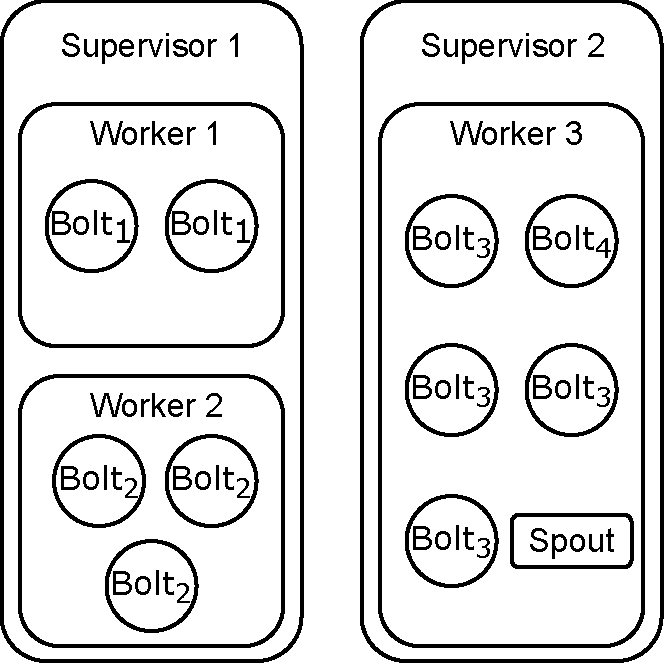
\includegraphics[width=0.45\textwidth]{figures/concepts/Storm-Physical.pdf}
     \caption{Storm physical architecture.}
     \label{fig:storm-physical}
\end{figure}

\subsubsection{Architecture}

For coordination between \textit{Nimbus} and the \textit{Supervisors}, \textit{Storm Cluster} uses \textit{Zookeeper}. Additionally, the states of the latter are stored in \textit{Zookeeper} or on a local disk, to provide fault tolerance in case of node failure.

Finally, \textit{Storm} architecture comprises \textit{Storm Cluster} and \textit{Zookeeper} cluster as shown by Figure \ref{fig:storm-architecture}.

\begin{figure}[!ht]
     \centering
     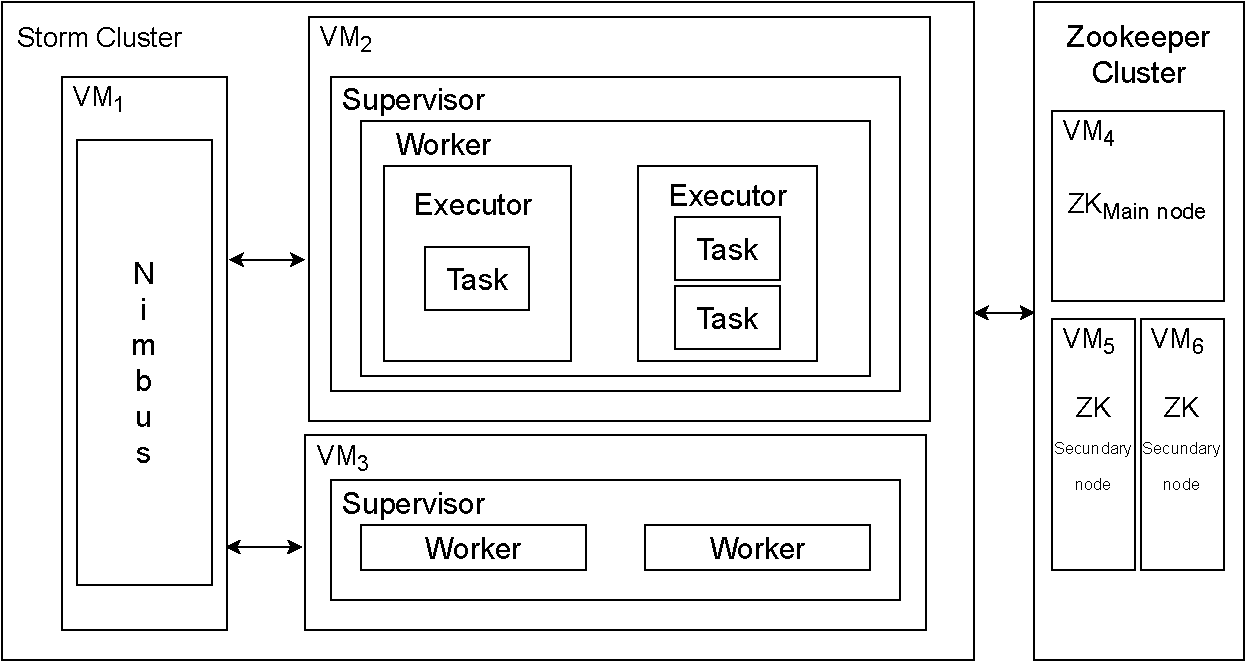
\includegraphics[width=0.8\textwidth]{figures/concepts/Storm-Architecture.pdf}
     \caption{Storm architecture.}
     \label{fig:storm-architecture}
\end{figure}

\subsection{Flink}
Flink \cite{Katsifodimos2016Flink} is a distributed SPS framework implemented in Java and Scala that enables the processing of unbounded data streams. It was initially developed by TU Berlin, and is currently part of the Stratosphere project.

\subsubsection{Logical architecture}

Like \textit{Storm}, a \textit{Flink Application} is a DAG. There are two types of components in a \textit{Flink Application}: \textit{Sources} and \textit{Operators}.

\textit{Sources} are the components necessary for sending external data to \textit{Flink Application}. Each \textit{Source} can be associated with logs, written data to external sinks, message queues, and interface with other systems. In this way, a \textit{Flink Application} can have one or more Sources in the data processing.

\textit{Operators} are the components that process the data in the \textit{Flink application} pipeline. Unlike \textit{Storm}, \textit{Flink} provides a high-level model, providing several default functions, which can be used. In this way, the system provides a high level of abstraction, simplifying various aspects of application construction. Like \textit{Storm}, each \textit{Operator} can be parallelised according to the application's requirements.

\begin{figure}[!ht]
    \centering
    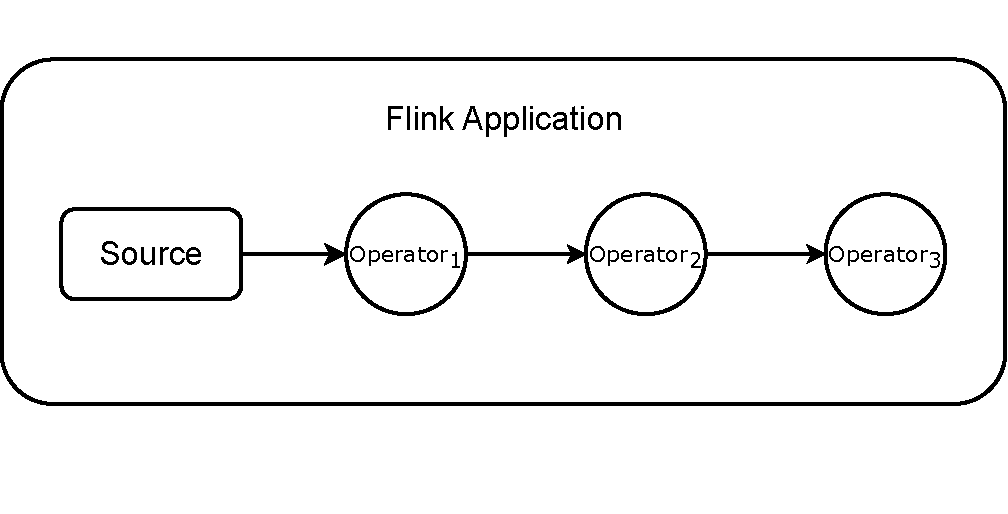
\includegraphics[width=0.75\textwidth]{figures/concepts/Flink-Logical.pdf}
    \caption{A Flink \textit{Topology}.}
    \label{fig:flink-logical}
\end{figure}

Figure \ref{fig:flink-logical} shows a \textit{Flink Application} (DAG) example, composed of a \textit{Source}, and three \textit{Operators}. In this example, can observe that the first \textit{Operator} performs the mapping task, while the second \textit{Operator} groups by a key and operates in a time window. These \textit{Operators} are named \textit{Transformation Operators}. After, the third \textit{Operator}, the last one, sends the processed data to either a database or an external system. This type of \textit{Operator} is called \textit{Sink Operator}.

\subsubsection{Physical architecture}

A \textit{Flink application} is deployed on \textit{Flink Cluster}, which has two components: \textit{Job Manager} and \textit{Task Manager}.

The \textit{Job Manager} is responsible for distributing and coordinating the execution of the \textit{Flink Application}. It decides on which machine each \textit{Task} will be deployed. At the same time, it monitors the status of the tasks, in case of a possible failure or progress in the stream, as well as the coordination of checkpoints and their recovery.

\textit{Task Manager} is the component that hosts one or more \textit{Tasks} of \textit{Flink Application}. Each \textit{Task} is associated to an \textit{Operator}, so this component must also allocate resources for its parallelisation. It also sends the state of the \textit{Tasks} to the \textit{Job Manager}.

Outside the \textit{Flink Cluster}, there is a component named \textit{Client}, which is responsible for the code of the \textit{Flink application} and for sending it to the \textit{Job Manager} for deployment. This component also receives statistics, results and the state of the execution of \textit{Flink Application}.

\begin{figure}[!ht]
     \centering
     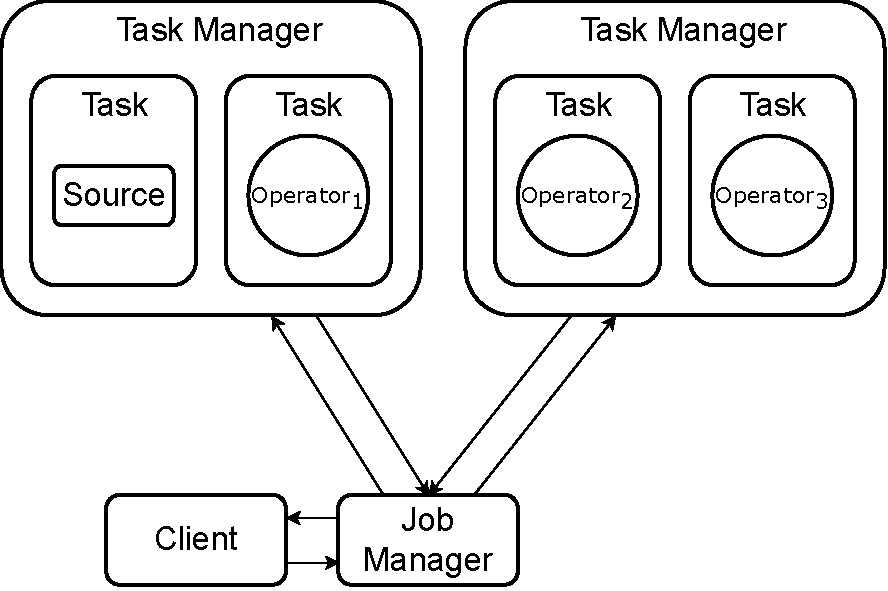
\includegraphics[width=0.7\textwidth]{figures/concepts/Flink-Physical.pdf}
     \caption{Flink physical architecture.}
     \label{fig:flink-physical}
\end{figure}

Figure \ref{fig:flink-physical} shows the scheduling of the \textit{Flink Application} (shown in Figure \ref{fig:flink-logical}) in a physical platform. According to some scheduling algorithms, each \textit{Operators} is placed in an available \textit{Task}.

\subsection{Discussion}
Although there are differences at the programming level, because \textit{Storm} does not provide a high level of abstraction as \textit{Flink}, both the logical and physical architecture are quite similar. On the one hand, the logical architecture is based on a DAG model, where each vertex is a component that performs a function and the edges are the data stream. As for the physical architecture, both are based on a model of main and secondary nodes, whereby the former is in charge of distributing the DAG as well as monitoring its state, and the later are responsible for processing the data.

It is worth noting that while we have given two examples, there have been other SPS frameworks, such as \textit{Apache S4} \citep{NeumeyerRNK10}, \textit{Apache Heron} \citep{KulkarniBFKKMPR15} or \textit{Apache Apex} \citep{GundabattulaW19}, but they have been given up over time. One of the main reasons is the flexibility provided by cloud services such as \textit{Amazon Web Services}, \textit{Google Cloud Platform} or \textit{Microsoft Azure}, where they provide their own SPS (\textit{Amazon Kinesis Data Streams}, \textit{Google Cloud Dataflow} and \textit{Microsoft Azure Stream Analytics}), with a high level of abstraction, simplifying both deployment and programming.

\section{Conclusion}
In this chapter, we present the concepts used in an SPS, as well as its requirements. We have explained each component, i.e. \textit{Stream}, \textit{Operator}, and \textit{Tuple}, and the concept of \textit{DAG}, which is the theoretical basis of the paradigm. In addition, we explained the parallelism of the operators, detailing their implementation and replication, as well as the types of \textit{Operator}, \textit{stateful} and \textit{stateless}, which are differentiated by the state handling in them. Finally, we present two SPS frameworks, \textit{Storm} and \textit{Flink}, explaining both their logical and physical architecture, as well as a discussion of the differences and similarities between them.
% !TEX root = ../main.tex
%
\chapter{Related work on adaptive| SPS}
\label{related-work}
One of the challenges of SPS is the dynamic availability resources. For example, if the external data source has an exponential increase of data, its transmission rate will increase considerably, so that the resources (either logical or physical) might be insufficient for processing all the data. One solution is to modify the amount of logical resources (operators) to maintain stable SPS performance. The works presented below focuses on the operator scaling.

This chapter presents two types of SPS adaptation: \textit{manual} and \textit{automatic}. The first one, as the name suggests, must be done manually by a user. The second one provides automatic scalability, being, thus, capable of modifying resource allocation according to the needs of the application. There are two approaches to \textit{automatic adaptation}: \textit{reactive} and \textit{predictive}.

\section{Manual adaptation}
\label{rw-manual}
One of the requirements of an SPS is its scalability when the load increases. The distribution of the application across nodes and the parallelisation of its tasks need then to be adapted.

\begin{figure}[!ht]
\begin{center}
\subfloat[Request for SPS reconfiguration.]{
  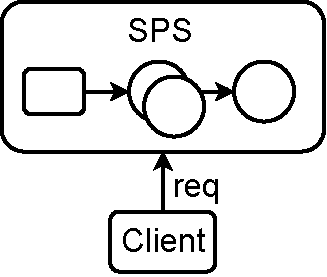
\includegraphics[scale=0.85]{figures/concepts/RW-Manual-1.pdf}
  \label{fig:manual-adaptation-1}
} \hspace*{1.5cm}
\subfloat[Response of SPS reconfiguration.]{
	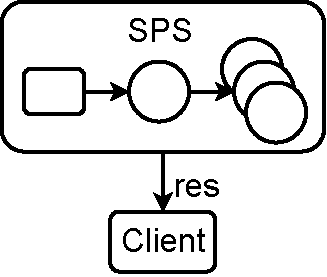
\includegraphics[scale=0.85]{figures/concepts/RW-Manual-2.pdf}
    \label{fig:manual-adaptation-2}
}
\caption{Manual adaptation of a SPS.}
\label{fig:manual-adaptation}
\end{center}
\end{figure}

The SPS frameworks mentioned above (see Section \ref{sps-frameworks}) provide both features, as well as the modification of their parallelisation through a client as shown in Figure \ref{fig:manual-adaptation}. Figure \ref{fig:manual-adaptation-1} shows the request to modify the parallelisation of a SPS, and then in Figure \ref{fig:manual-adaptation-2}, once the modification has been performed, the response that the modification has been successful is sent to the client.

Basically, there are two ways to manually modify resources: GUI application or terminal command. In both cases, the parallelisation degree of the components must be indicated. For \textit{Storm}, the number of \textit{Executors} per \textit{Bolt} and the number of \textit{Workers} must be informed. While for \textit{Flink} it is necessary to inform, the degree of parallelisation of each \textit{Operators} and the number of \textit{Tasks}. In both SPS framworks, reconfiguration requires stopping the application and restarting it. A comparative summary of the two is presented in Table \ref{tab:manual-adaptation}.

\begin{table}[!ht]
\begin{tabular}{|l|l|l|l|l|l|}
\hline
Framework & Client                                                       & \begin{tabular}[c]{@{}l@{}}Mod. of\\ operators\end{tabular} & \begin{tabular}[c]{@{}l@{}}Mod. of\\ nodes used\end{tabular} & \begin{tabular}[c]{@{}l@{}}Reconf.\\ downtime\end{tabular} & \begin{tabular}[c]{@{}l@{}}State\\ restoration\end{tabular} \\ \hline
Storm     & \begin{tabular}[c]{@{}l@{}}GUI /\\ Terminal cmd\end{tabular} & Yes                                                                 & Yes                                                                  & Yes                                                        & Manual                                                      \\ \hline
Flink     & \begin{tabular}[c]{@{}l@{}}GUI /\\ Terminal cmd\end{tabular} & Yes                                                                 & Yes                                                                  & Yes                                                        & Automatic                                                   \\ \hline
\end{tabular}
\caption{Comparison of manual adaptation of SPS.}
\label{tab:manual-adaptation}
\end{table}

To cope with such a manual intervention drawback, ELK Stack \cite{HasaniF18} proposes to read the SPS statistics and notify the user if the system is overloaded, aiming at helping him/her to decide on the system reconfiguration. Although this alert system indicates an overload in the system, the logic of the application or the system parameters remain dependent on the user's expert knowledge, which is a limitation of this solution.

\section{Automatic adaptation}
\label{rw-auto}
As a consequence of the limitations manual adaptation, some works have proposed self-adaptive SPSs \citep{KahveciG20, arkian2021model} by modifying the amount of resources aiming at increasing the performance of the system and/or decreasing the costs associated with excessive idle resources. The works that follows are able to automatically modify the allocated resources in order to satisfy the requirement of instantaneous processing and response.

In general, this type of adaptation is achieved by using SPS statistics, through a monitoring system. Unlike \textit{manual adaptation}, which is passive since it depends on a user to perform the adaptation, \textit{automatic adaptation} actively and constantly analyses the SPS. Figure \ref{fig:automatic-adaptation} presents the gathering of statistics by the monitor, which are performed according to some set of parameter (number of messages processed, time windows, etc.). Subsequently, the model in charge of the automatic adaptation determines that a new configuration is needed, so it actively signals this change to the SPS.

\begin{figure}[!ht]
	\centering
	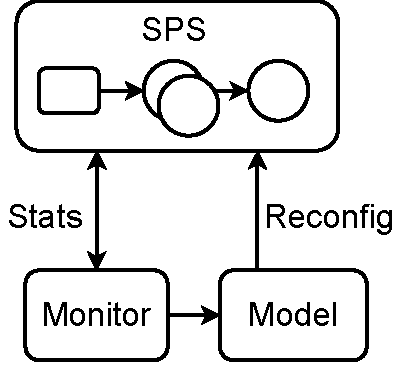
\includegraphics[scale=0.85]{figures/concepts/RW-Automatic.pdf}
	\caption{Automatic adaptation in a SPS.}
	\label{fig:automatic-adaptation}
\end{figure}

Existing works apply either a reactive or predictive approach to implement an adaptive SPS. The \textit{reactive approach} corresponds to adaptations that are performed \textit{in situ}, i.e. it considers the states or/and variables of the system to determine whether it is necessary to adapt the system. This approach considers algorithms focused on modifying the system as a response to its current state, based on metrics and thresholds. On the other hand, the \textit{predictive approach} analyses the history of the states and/or variables system to give a proposal of a new configuration based on prediction models. Therefore, more complex systems such as Machine Learning, time series, or mathematical models are used to determine the proposed configuration.

\subsection{Reactive approach}
\label{rw-auto-reactive}
The \textit{reactive approach} is based on state analysis via a monitor, which periodically receives system statistics (utilization, queue size, throughput, CPU utilisation, etc.). These statistics determine an objective function, so that if their value exceeds a threshold, the system will modify the number of replicas of the operators.

Figure \ref{fig:rw-reactive-threshold} presents a variation of the objective function, which over time changes the state of the system. Consider that the used metric is the workload. If the metric value is lower (resp., higher) than the lower threshold (resp., upper threshold), the system is considered underloaded (resp., overloaded). And in the case where the value of the metric is between the lower and upper threshold, the system is considered stable.

\begin{figure}[!ht]
	\centering
	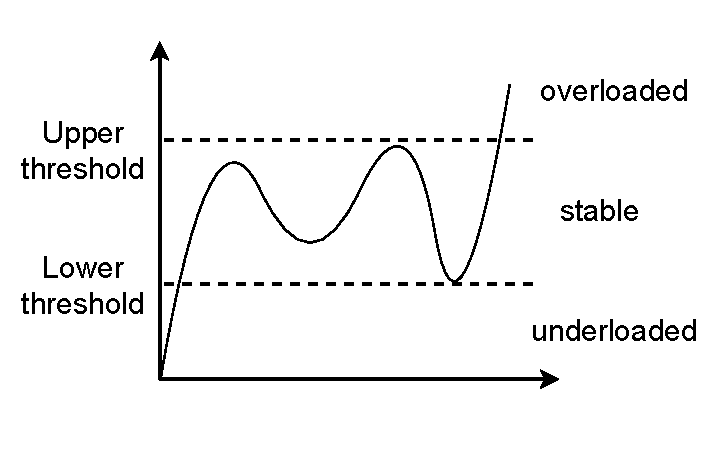
\includegraphics[scale=0.75]{figures/concepts/RW-Reactive-Threshold.pdf}
	\caption{Thresholds in a reactive model.}
	\label{fig:rw-reactive-threshold}
\end{figure}

Once the state of the system is determined, if an instability happens (e.g. overloaded or underloaded), the reactive model proposes a new configuration. Figure \ref{fig:rw-reactive} shows an example of a SPS, which uses a \textit{reactive approach}. The metric determines the state of the system according the thresholds. Therefore, if the system is unstable, the model proposes a new configuration, which modifies the number of replication of the operators according to the needs. Otherwise, no configuration is proposed.

\begin{figure}
	\centering
	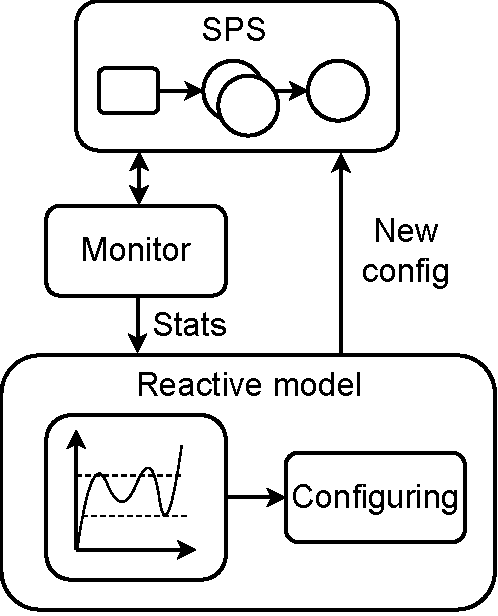
\includegraphics[scale=0.85]{figures/concepts/RW-Reactive.pdf}
	\caption{Adaptive SPS using a \textit{reactive approach}.}
	\label{fig:rw-reactive}
\end{figure}

\textit{StreamCloud} \citep{GulisanoJPSV12} is an adaptive SPS, based on Borealis SPS \citep{AbadiABCCHLMRRTXZ05}, that modifies the number of replicas in the system according to CPU utilisation. Depending on the number of queries issue to the system, the number of operators processing the requested tasks increases or decreases. For this, a specific operator, called \textit{slit}, distributes the data, and an other one, called \textit{merge}, gathers the information delivered by the operator’s replicas. So this system only supports certain operations, so that \textit{split} and \textit{merge} operators are automatically created. In this way, there are no problems with stateful operators, such as counters and sorting algorithms, since it automatically performs the procedure of separation and union of data.

The MEAD SPS \cite{RussoCCP21} was implemented in Flink \cite{CarboneKEMHT15}. Operator auto-scaling takes place based  Markovian Arrival Processes approach, where the system load is analysed according to a queuing model. The SPS proposes a MAPE-K for the control flow. Evaluation experiments were carried out on both synthetic and real environments. However, if the authors state that MEAD supports operators scaling-out, such a feature has not been implemented. On the other hand, similar to other works that use Flink, such as \cite{arkian2021model}, reconfiguration induce performance degradation.

Enorm \citep{MadsenZS16}, a work based on Storm, proposes elasticity that integrates with fault tolerance. For this, it uses a check-pointing mechanism to enable fast and low-cost state migration by increasing or decreasing parallelism. This work focuses on how to adapt the system by increasing or decreasing parallelism, but not on the amount of parallelism required by the system. In addition, the work uses a threshold-based approach to determine when to scale. We believe the author's proposal can be integrated into our solution to provide integrity when replicating stateful operators.

Some works also focus on the dynamic adaptation of SPS under a reactive approach, with the difference that they use their own SPS. For instance, the SPS Joker, which claims to provide elasticity with ``organic'' adaptation, is presented in \cite{KahveciG20}. The authors denote ``organic adaptation'', when the execution of streaming application scales safely, transparent, dynamic, and automatic. Joker continuously monitors the runtime performance of the SPS and runs optimization algorithms to resolve bottlenecks, using the throughput metric as an objective function. It then scales the application by adjusting the degree of pipeline and data parallelism. While parallelising SPS tasks, distribution between machines has not been implemented.

Other works such as \citep{GedikSHW14, SchneiderAGBW09} also use parallel elastic tasks and a metric (the throughput in both works) for determined the state of each task, and, the SPSs are deployed in the {Cloud}. Therefore, parallelization of tasks uses different VMs. Other similar work, \citep{FernandezMKP13} propose to increase the number of replicas from the operators to reduce bottlenecks, where each replica is hosted in a VM. For the detecting bottlenecks, a monitor inquires the state of each operator from time to time. If an operator exceeds the established load threshold on the CPU usage, it is replicated.

In Esc \citep{SatzgerHLD11} the authors proposed to dynamically modify the replicas of the operators, as well as to couple and release machines to adjust the computational capabilities to the current nodes. To determine the number of replicas of the operators, the latency of the system is analyzed and the modification of replicas is determined according to thresholds. In the case of machines, their respective workload is used. Thus, the Esc implementation provides elasticity of both physical and logical resources automatically.

Another work that uses threshold-based decisions for operator replica adaptation is \citep{HeinzeJHF14}. The authors compared decisions based on local thresholds on the processing operators, global thresholds of the system, and a reinforcement learning approach. Besides lower and upper bounds a target utilization value is taken into account. A grace period after a scaling decision is considered in order to maintain stability. The reinforcement learning approach uses the actions: scaling up, scaling down, and no action. The system uses as reward a weighted average of the difference between the current value and respective target system utilization. 

Flood \citep{AlvesBM10} proposes a DPS (Distributed data stream processing) which, while modifying the replicas of the operators, is determined according to the physical resources. To this end, a manager module gathers runtime statistics such as the amount of used CPU, latency or available memory of the VMs. These statistics make it possible to see in which load range the machine can be placed, according to the established thresholds, in order to subsequently modify the VMs. Thus, by increasing (resp. decreasing) the VMs, the replicas associated with the VM are also added (resp. removed). 

To this end, above works presented use only one metric, which does not take into account the behaviour of other variables, either local (operators) or global (SPS). %Therefore, the aim of our \textit{reactive model} is to analyse the state of the system at the moment from different perspectives, considering the multiple factors of the environment.

Table \ref{tab:rw-reactive} shows a comparison of the discussed adaptive SPSs that use a reactive approach. \textit{Objective} and \textit{Model} are the objective function and model used for adaptation respectively. \textit{VM Scaling} indicates whether it uses horizontal or vertical scalability of the physical resources (VMs). \textit{Stateful operator} indicates whether the SPS supports type of operator. Then the \textit{Infrastructure} used for its deployment is indicated. Finally the used \textit{SPS framework}, \textit{None} means that the work does not use any framework, because it has implemented its own SPS.

\begin{table}[!ht]
\centering
\begin{tabular}{|c|c|c|c|c|c|c|}
\hline
\rotatebox[origin=l]{90}{Reference}	& \rotatebox[origin=l]{90}{Objective}  & \rotatebox[origin=l]{90}{Model} & \rotatebox[origin=l]{90}{VM Scaling} & \rotatebox[origin=l]{90}{Stateful Operator} & \rotatebox[origin=l]{90}{Infrastructure} & \rotatebox[origin=l]{90}{SPS Framework} \\
\hline
\citep{GulisanoJPSV12} & CPU & Threshold & Non & Yes & Cloud & Borealis\\
\hline
\citep{RussoCCP21} & Throughput & Regression & Yes & Non & Cluster & Storm \\
\hline
\citep{MadsenZS16} & Latency & Threshold & Non & Yes & Cloud & Storm\\
\hline
\citep{KahveciG20} & Throughput & Heuristic & Non & Yes & Single Machine & None\\
\hline
\citep{GedikSHW14} & Throughput & Threshold & Non & Yes & Cluster & None \\
\hline
\citep{SchneiderAGBW09} & Throughput & Heuristic & Non & Non & Single Machine & None \\
\hline
\citep{FernandezMKP13} & Throughput & Threshold & Yes & Yes & Cloud & None \\
\hline
\citep{SatzgerHLD11} & Latency & Threshold & Non & Non & Cluster & None \\
\hline
\citep{HeinzeJHF14} & Latency & Heuristic & Yes & Yes & Cluster & None \\
\hline
\citep{AlvesBM10} & CPU, Network & Threshold & Yes & Non & Cloud & None \\
\hline
\end{tabular}
\caption{Comparative table of adaptative SPS that use reactive approach.}
\label{tab:rw-reactive}
\end{table}

\subsection{Predictive approach}
\label{rw-auto-predictive}
The \textit{predictive approach} is based on prediction of the future behaviour of an SPS to determine its new configuration. For this, its behaviour is estimated according to some predictive model based on its history. Examples of such models are regressions, time series, neural networks, etc. Data used for prediction can be system statistics, such as CPU utilisation, latency, throughput, etc.

Figure \ref{fig:rw-predictive} shows an example of a \textit{predictive approach}, where the system analyses CPU utilisation. With the sample history of this statistic, a prediction is made about the future behaviour of the system based on some predictor. Finally, based on the prediction, the model determines a possible state of the SPS, and if necessary, mitigate the possible CPU overloads.

\begin{figure}[!ht]
	\centering
	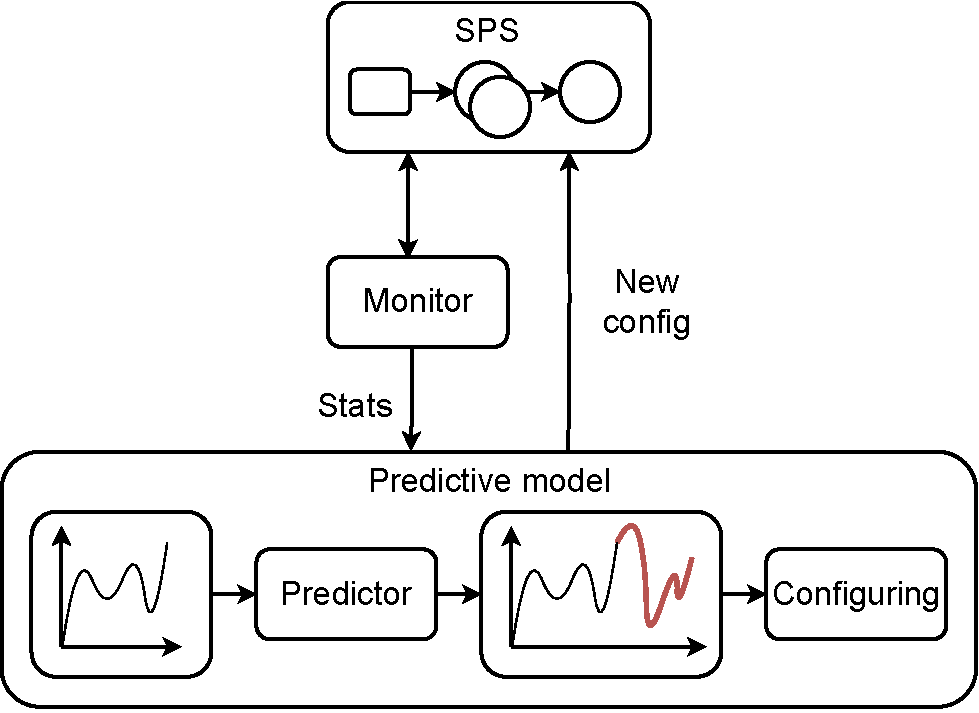
\includegraphics[scale=0.7]{figures/concepts/RW-Predictive.pdf}
	\caption{Predictive model of an adaptative SPS.}
	\label{fig:rw-predictive}
\end{figure}

In \cite{CardelliniPNR18}, the authors  propose a hierarchical decentralized adaptive SPS in \textit{Storm}, using the MAPE model to design the solution. Regarding the scaling policy, the used metric is CPU utilization of the operator replicas, which defines whether a system adaptation is necessary or not. 
The proposed solution also analyzes the costs associated for each reconfiguration and on a latency-based reinforcement learning model to predict system behavior. One of the parameters is the downtime, i.e., the time necessary to restart the system which can induce much overhead. %Our SPS does not present such an overhead since inactive replicas are pre-allocated at the beginning of the SPS execution.

There also exist some works that use SPS frameworks, such as Gesscale which is implemented in Flink \cite{arkian2021model}. In this work, a model is proposed in order to compute the maximum processing capacity of a physical node. For this purpose, like our approach, the SPS defines multiple different metrics which are the maximum sustainable throughput capacity of a single node, maximum network delay, and parallelization inefficiency. By applying these metrics, the model analyzes the behavior of the system in every time window and, if necessary, modifies the replicas elastically. One of the disadvantages of Gesscale solution is that, for reconfiguring the system, it is necessary to restart the application, which takes a considerable time.

%%%% AUTOSCALE AND DABS-STORM
The authors in \cite{KombiLL17} present a predictive SPS called AUTOSCALE which analyzes the data stream to predict traffic congestion on tasks. Queue theory principle is applied for gathering information about utilization, arrival rate, and departure rate of the tasks. A centralized system then analyzes the statistics, predicting data congestion in tasks according to a sliding window. Whenever the system detects a possible congested operator, the number of replicas is increased. However, the article does not present evaluation results in scenarios with high variations in the data flow rate.

DABS-Storm, a congestion prevention SPS, is presented in \cite{KombiLLRB19}. Its aim is to reduce the degradation of the quality of the results. To this end, a metric is used to estimate the level of activity of the operators. A monitor gathers statistics about the operators activity and then, based on a metric, decides if the amount of resource allocated to each operator should be modified or not. Such a metric is defined by predicting the system input by using a regression function as well as taking into account pending events. The capacity of the operators is also estimated, considering both the physical capacity of the machine where the operator is located and the latency of the system. As DABS-Storm has been implemented in Storm, its operators reconfiguration approach carries the drawback of Storm reconfiguration downtime cost. 
%%%% AUTOSCALE AND DABS-STORM

ELYSIUM \cite{LombardiABQ18} is a Storm-based SPS that scales in and out
the number of replicas of the operators and, if necessary, modifies the number of workers associated with the application (horizontal and vertical scalability). It provides both a reactive and predictive approach based on time window and an ANN model. ELYSIUM was not been evaluated with a real prototype integrated in Storm.

The authors in \cite{BalkesenTO13} propose a predictive model implemented in Borealis SPS \cite{AbadiABCCHLMRRTXZ05}, taking into account not only the input rate as a metric, but also the capacity of the nodes as well as data processing complexity. Then, the model provides an equation that characterizes the workload of the system and determines the amount of required parallelism for processing events. Therefore, its objective is both the balance of the workload between the nodes and the reduction of latency. Although the system is capable of scaling-out, it does not perform scale-in, so it does not consider the reduction of allocated resources.

Based on look-ahead approach, PLAStiCC is a predictive scheduling proposed by \cite{KumbhareSP14}. Its model analyzes the system performance through the balance of resource overload. Furthermore, as it is conceived to run on clouds, allocated resources can have different costs. Therefore, the model considers not only the workload of the system, but also the costs associated with the increase in resources. The work is not evaluated in a real platform, nor does it use a real application, because it uses for evaluation the cloud simulator CloudSim \cite{Calheiros2009CloudSim}, as well as synthetic dataflows.

The Elastic-PPQ SPS \cite{MencagliTD18} proposes to analyze the system at short-term and medium/long-term levels. The first one performs an analysis on the events that arrive in a time interval while the second one takes into account longer periods to perform a more complex analysis, using Fuzzy Logic Controller.  To this end, an autonomous system, based on QoS, manages the system resources according to a runtime strategy, which considers the complexity of the system components. In this way, the parallelism of the tasks, associated with a set of threads, can increase or decrease. For the evaluation and validation of system load analysis, both synthetic and real data were used. Although the solution is quite robust, since it is implemented in FastFlow \cite{aldinucci2017fastflow} framework, its focus is more on high performance processing than on distributed data processing.

Finally, \cite{HidalgoCR17} performs an analysis of operator replicas based on queue theory. Operator utilization due to data arrival and departure rates is used as a metric, which determines the state of the operator, thus modifying the number of its replicas, if necessary. The solution uses a hybrid approach, composed of a predictive approach, based on Markov chains, and a reactive one, based on thresholds. The aim of the former is to analyse possible system behaviours, and the latter is to adjust the system configuration in short periods of time.

Table \ref{tab:rw-predictive} shows a comparison of adaptive SPSs using predictive approach. \textit{Objective} and \textit{Model} are the objective function and predictive model used for adaptation. \textit{VM Scaling} indicates whether it uses horizontal or vertical scalability of the physical resources (VMs). \textit{Stateful operator} indicates whether it supports this type of operator. Then the \textit{Infrastructure} used for its deployment is indicated. Finally, the \textit{SPS framework} used. \textit{None} means that a frameworks is not used, because it implemented its own SPS.

\begin{table}[!ht]
\centering
\begin{tabular}{|c|c|c|c|c|c|c|}
\hline
\rotatebox[origin=l]{90}{Reference}	& \rotatebox[origin=l]{90}{Objective}  & \rotatebox[origin=l]{90}{Model} & \rotatebox[origin=l]{90}{VM Scaling} & \rotatebox[origin=l]{90}{Stateful Operator} & \rotatebox[origin=l]{90}{Infrastructure} & \rotatebox[origin=l]{90}{SPS Framework} \\
\hline
\citep{CardelliniPNR18} & Latency & \begin{tabular}[c]{@{}l@{}}Reinforcement\\ learning\end{tabular} & Non & Yes & Cluster & Storm \\
\hline
\citep{arkian2021model} & Throughput & Model-based & Yes & Yes & Cluster & Flink \\
\hline
\citep{KombiLLRB19} & Throughput & Time series & Non & Yes & Cluster & Storm \\
\hline
\citep{LombardiABQ18} & Utilization & ANN & Yes & Yes & Cluster & Storm \\
\hline
\citep{BalkesenTO13} & Utilization & Heuristic & Non & Non & Cluster & Borealis \\
\hline
\citep{KumbhareSP14} & Throughput & Heuristic & Non & Non & Simulation & None \\
\hline
\citep{MencagliTD18} & Throughput & Fuzzy logic & Non & Non & Single Machine & FastFlow\\
\hline
\citep{HidalgoCR17} & Throughput & Markov Chain & Non & Non & Cluster & S4 \\
\hline
\end{tabular}
\caption{Comparative table fo adaptative SPS that use predictive approach.}
\label{tab:rw-predictive}
\end{table}

\section{Conclusion}
This chapter has presented several works on the adaptation of the number of operator replicas of an SPS, specifically the number of replicas of each operator in a DAG SPS.

First, we present the manual adaptation of two popular \textit{SPS frameworks}, \textit{Storm} and \textit{Flink}, that allows the modification of their respective resources. Although they provide a way for reconfiguring a SPS, the solution depends on a user for adaptation. In addition, both frameworks have a downtime when modifying their configurations, which is an important limitation to consider.

Subsequently, we analyse automatic adaptation solutions, which is can be divided into two approaches: reactive and predictive. The ones based on reactive approach generally focus on metrics thath either considerer one variable on multiple variables whose relevance for decision can not be configured. These based on the predictive approach mostly use a \textit{SPS framework}, which present performance degradation when modifying resources, given that there is a downtime of the system. Furthermore, they usually use only one predictive model, and the result may vary depending on the workload scenario.

% !TEX root = ../main.tex
%
\chapter{Proposed adaptive SPS}
\label{solution}
In this chapter, we present our self-adaptive SPS capable of providing high throughput, scalability, and low latency, while guaranteeing the integrity of the results obtained from the analysed data. Our proposal, which is an extension of \textit{Storm}, dynamically adapts the number of operator replicas to cope with environments that present highly variable input rate environments.

This chapter is structured in three sections. Section \ref{modified-sps} presents the extensions made in \textit{Storm} to circumvent its limitations. Then, Section \ref{reactive-approach} presents \rSPS{}, our proposed \textit{reactive approach}, published in \citep{WladdimiroNCA}, which is based on multi-metrics. Finally, Section \ref{predictive-approach} presents \pSPS{}, our \textit{predictive approach}, published in \citep{WladdimiroSBAC}, which focuses on predicting the number of replicas required by for the next time interval.


\section{New features of the adaptive SPS}
\label{modified-sps}
Most SPSs require expert knowledge for configuring the system's processing resources according to the environment requirements. Furthermore, they can not reconfigure themselves at runtime. Highly variable input rate environments may induce resource over-provisioning, wasting processing resources, while under-provisioning, may induce the loss of data processing.

In order to handle such scenarios, \rSPS{} and \pSPS{} can dynamically allocate/deallocate operators' replicas at runtime. Such an elasticity enables the two adaptive SPSs to adapt their processing logic, optimizing resource usage while minimizing data loss.

Both SPSs exploit two mechanisms that do not exist in the original \textit{Storm}: a pool of replicas and a \textit{load-aware} grouping strategy. The first one attempts to reduce adaptation reaction delay reducing, therefore, event processing latency. \textit{Storm}'s original version provides a rebalancing feature to reallocate the number of executors for a bolt. However, this action involves system downtime, loss of messages, and increasing of end-to-end latency which degrades performance. The second mechanism handles operators' replicas event distribution. Grouping strategies in \textit{Storm} define how events are distributed among operators. Due to the heterogeneous nature of the processing resources and operators' tasks complexity, balance issues may occur, creating bottlenecks and increasing latency.

\subsection{Pool of replicas}
\label{pool}

At initialization, \rSPS{} and \pSPS{} assign, for each operator, a pool of replicas deployed by the scheduler. Replicas can be either in  \textit{active} or \textit{inactive} state. The state of a replica can be modified at runtime. An inactive (resp., active) replica consumes negligible (resp., non negligible) CPU power and can be dynamically activated (resp., deactivated) whenever the prediction model of the system detects the need for increasing (resp., decreasing) the replicas for the operator in question. Thus, based on the number of available cores by VMs and the fact that, in general, each replica is associated with a thread, it is possible to set the size of a pool ($p$), which is the same for each operator pool. 

Figure \ref{fig:pool} considers a DAG with operators $O_A$ and $O_B$ and their respective pool of replicas of size $p$. When initialising the application, there is only one active replica per operator as shown in Figure \ref{fig:pool-without} there is only one active replica per operator ($O_{A.1}$ and $O_{B.1}$). Therefore, the other replicas are inactive and do not receive a data stream. It is important to note that it is necessary to keep one replica active, since if all replicas are inactive, the DAG components related to the operator would be lost. The state of an operator can be modified, as is the case of $O_{A.2}$, which changes from inactive to active as shown in Figure \ref{fig:pool-with}. When this is done, the stream data sharing is determined by the grouping strategy of the operator (see Section \ref{grouping}).

\begin{figure}[!ht]
\begin{center}
\subfloat[One active replica per operator.]{
  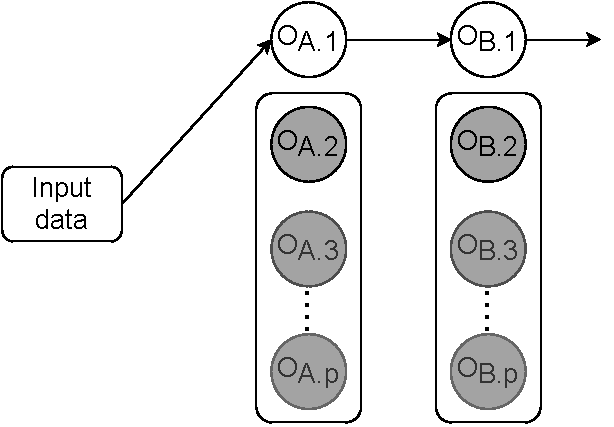
\includegraphics[width=0.5\textwidth]{figures/concepts/ASPS-PoolReplica-1.pdf}
    \label{fig:pool-without}
}
\subfloat[Activation of a replica.]{
	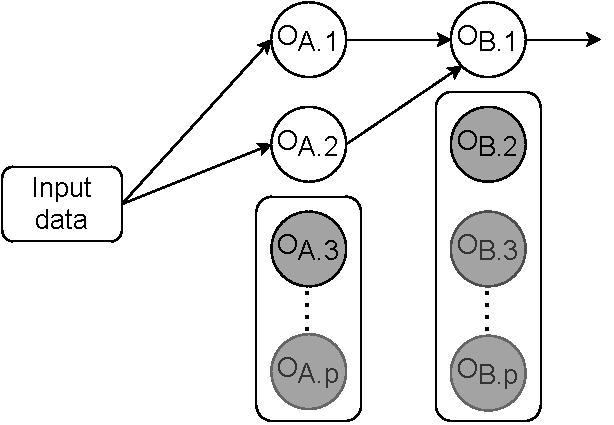
\includegraphics[width=0.5\textwidth]{figures/concepts/ASPS-PoolReplica-2.pdf}
    \label{fig:pool-with}
}
 \caption{Example of pool replicas for two operators.}
    \label{fig:pool}
\end{center}
\end{figure}

Despite its simplicity, performance results showed that the pool of replica is very effective, since \rSPS{} and \pSPS{} are self-adaptive at runtime at a negligible cost. Moreover, as it is implemented in \textit{Storm}, there is no need to restart the application, so downtime is avoided.

\subsection{Load-Aware Grouping}
\label{grouping}
A grouping technique specifies how a stream (tuples) should be partitioned among operators. Using traditional methods like \textit{Shuffle grouping} (see Section \ref{grouping}), tuples are randomly distributed across operators, ensuring that each operator receives an equal number of tuples. Due to the complexity of the tasks or the heterogeneous nature of the processing resources, load balance issues may occur. In this case, while pending events are still in the processing queue, new events can go on arriving. 

To overcome this problem, we propose a \textit{load-aware grouping} strategy, which considers the load state of active replicas in terms of $\mu_{i.j}(t)$, i.e., the number of events processed by replica $j$ of an operator $i$ during a time interval $t$, $et_i$, the average execution time of one event at operator $i$, and $td$, the time interval duration. Note that we define a replica $j$ of an operator $i$ as $O_{i.j}$.

Therefore, the proportional distribution of events considers the current utilization of active replicas. The utilization is computed following Equation \ref{eq:utilization}, where $U$ ranges between $0$ and $1$ for a replica $j$ of an operator $i$. A $0$ and $1$ values represent $0\%$ and $100\%$ utilization of the replica respectively. If all replicas present the same utilization value, events are sent in a round-robin fashion. Otherwise, events will be assigned to the replica with  the lowest load.

\begin{equation}
\label{eq:utilization}
    U_{i.j}(t) = \frac{\mu_{i.j}(t) \times et_i}{td}
\end{equation}

Algorithm \ref{alg:grouping} shows the pseudo-code of the \textit{load-aware grouping} strategy. The loop of lines 3-7 is responsible for selecting the replica $j$ of operator $O_i$ with the lowest utilisation. Then, if the utilisation is $100\%$ ($U=1$), which means that all the replicas are overloaded, a replica candidate is randomly chosen (lines 8-9). Otherwise, the overhead of processing the event is added to the replica candidate utilisation (line 11). Finally in line 13, the event is sent to the replica candidate of the $O_i$ operator.

\begin{algorithm}
\caption{Load-Aware grouping for operator $O_i$.}
\begin{algorithmic}[1]
 	\REQUIRE Statistics of replicas of $O_{i}$ in interval $t$.
 	\ENSURE Replica $O_{i.m}$ that should process the event.
 	\STATE {$m \gets 0$}
 	\STATE {$p \gets$ sizePoolReplicas($O_i$)}
 	\FOR {$j : 1 \to p$}
 	    \IF {$U_{i.j} < U_{i.m}$}
 	        \STATE {$m \gets j$}
 	    \ENDIF
 	\ENDFOR
 	\IF {$U_{i.m} = 1$}
  	    \STATE {$m \gets$ getReplicaRoundRobin($O_{i}$)}
  	\ELSE
  	    \STATE $U_{i.m} \gets U_{i.m} + \frac{et_i}{td}$  
 	\ENDIF
 	\STATE sendEvent($O_{i.m}$)
\end{algorithmic}
\label{alg:grouping}
\end{algorithm}
\section{Reactive approach}
\label{reactive-approach}
Due to the high variability of the input rate, the adaptation of SPS resources is necessary for performance sake. In this first proposal, denoted \rSPS{}, we use a reactive model to analyse the state of the operators to modify the number of active replicas of the operators in the DAG. Table \ref{tab:rsps-notations} summarises all parameters used in \rSPS{}.

\begin{table}[!ht]
\begin{tabular}{|c|l|}
    \hline
    \textit{\textbf{Parameter}}     & \textit{\textbf{Description}}             \\  \hline
    $O_i$			& operator $i$ \\
    $t$				& time interval number \\ 
    $td$			& time interval duration  \\
    $et_i(t)$		& average execution time of one event by $O_i$ during $t$ \\
    $et_i$		& average execution time of one event by $O_i$ according to the benchmark\\
    $q_i(t)$		& queue of events received and not processed by $O_i$ at the end of $t$ \\
    $\mu_i(t)$		& number of events processed by $O_i$ during $t$\\
    $r_i(t)$ 		& number of active replicas of $O_i$ during $t$ \\
    $U_i(t)$		& Utilization metric by $O_i$ during $t$ \\
    $E_i(t)$		& Execution Time metric by $O_i$ during $t$ \\
    $Q_i(t)$		& Queue metric by $O_i$ during $t$ \\
    $\delta_i(t)$	& State metric by $O_i$ during $t$ \\
    \hline
\end{tabular}
\caption{Parameters notation and their description in \rSPS{}.}
\label{tab:rsps-notations}
\end{table}


\subsection{Metrics}
An adaptive SPS should define metrics to characterize the state of the operators at runtime on a given scenario. Traditional metrics such as throughput, latency, and CPU are the most used in literature (see Section \ref{rw-auto-reactive}). In \rSPS{}, we propose to integrate the metrics denoted \textit{Utilization ($U$)}, \textit{Execution Time ($E$)}, \textit{Queue ($Q$)} and \textit{State} ($\delta$).

\textit{Utilization} metric  is defined by Equation \ref{eq:rsps-utilization}. The aim of the metric is to characterize the operator load: if its value is close to 1 (resp., 0), the operator is overloaded (resp., underloaded). Figure \ref{fig:prediction-replicas} shows an example composed of three independent operators ($O_1$, $O_2$, and $O_3$) that have different $U_i(t)$.

\begin{equation}
\label{eq:rsps-utilization}
        U_i(t) = \frac{\mu_i(t) \times et_i(t)}{r \times td}
\end{equation}

In Figure \ref{fig:rsps-metric-u}, the three operators have 2 replicas ($r_i=2$) and an average execution time of 200 milliseconds ($e_i=200~ms$). As the number of events processed is different during the time interval $t$ for each operator, their loads are different. $O_1$ has no idle time, so it is at maximum utilization, so the operator is overloaded. $O_2$ has a load level which is $50\%$ of the time idle in time period $t$. $O_3$ is almost underloaded.

\begin{figure}[!ht]
    \centering
    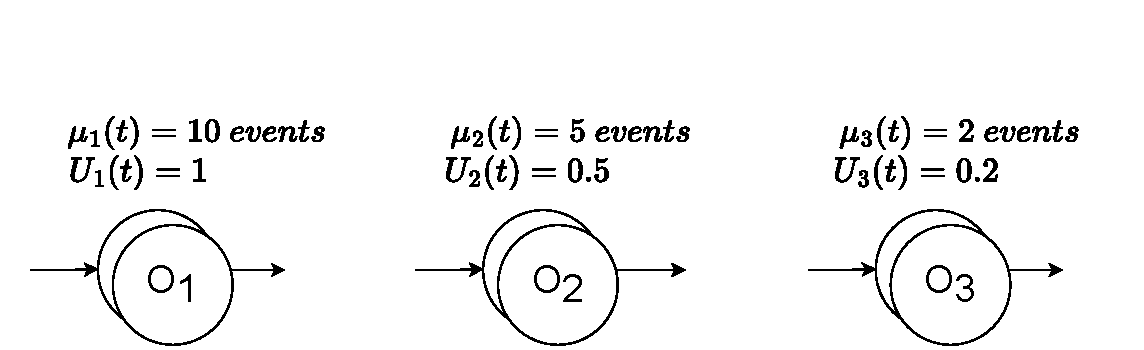
\includegraphics[width=0.8\textwidth]{figures/concepts/RA-SPS-Metric-U.pdf}
    \caption{Example of the \textit{Utilisation} metric.}
    \label{fig:rsps-metric-u}
\end{figure}


\textit{Execution Time} metric  is defined by Equation \ref{eq:rsps-latency}. The aim of the metric is to characterize execution degradation of operators: if the value of $et_i(t)$ is greater than $et_i$, the physical machines are overloaded. It is a QoS metric which allows to detect struggle operators. Therefore, the difference between $et_i(t)$ and $et_i$ is that the latter is the average execution time of one event processed by an operator $O_i$ without any extra load. The variable $et_i$ is considered as a baseline, and it is estimated by previously  benchmark execution.

\begin{equation}       
        E_i(t) = 1-\frac{et_i}{et_i(t)}
\label{eq:rsps-latency}
\end{equation}

In Figure \ref{fig:rsps-metric-e}, the three operators have an average execution time of 200 milliseconds ($et_i=100$). $O_1$ has a large extra load, possibly due to overutilisation of resources, so the execution time is much longer. Unlike $O_3$, which has no extra load, or $O_2$ which has less extra load.

\begin{figure}[!ht]
    \centering
    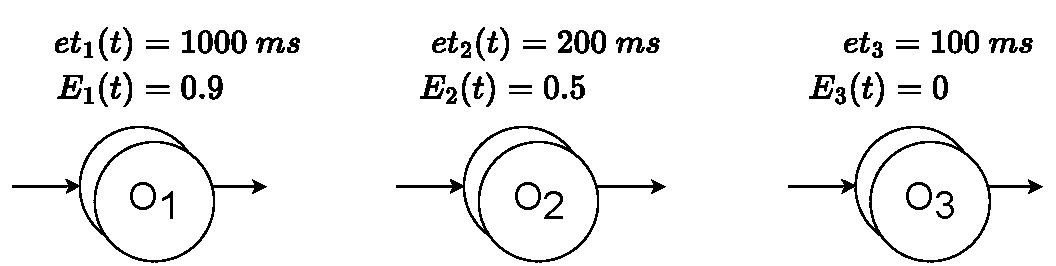
\includegraphics[width=0.8\textwidth]{figures/concepts/RA-SPS-Metric-E.pdf}
    \caption{Example of the \textit{Execution Time} metric.}
    \label{fig:rsps-metric-e}
\end{figure}

\textit{Queue} metric is defined by Equation \ref{eq:rsps-queue}. The aim of the metric is to analyze the impact of the input queue on the operator with respect to its current processing capacity. The $Q_i(t)$ tackles the input traffic behavior (traffic shape). Sudden peaks will increase the number of the events queued, $q_i(t)$ value, generating higher values of $Q_i(t)$. If $q_i(t)$ value is 0 or $Q_i(t)$ value is negative, its value is set to 0.

\begin{equation}
        Q_i(t) = 1-\frac{\mu_i(t)}{q_i(t).}
\label{eq:rsps-queue}
\end{equation}

In Figure \ref{fig:rsps-metric-q}, the three operators have 10 processed events ($\mu_i(t)=10~events$). In the case of $O_1$, it has a small tail, so its impact is minimal. Compared to $O_1$, $O_2$ has a larger number of queued events, which is reflected by the increase of metric value. Finally, $O_3$ has a considerable high $Q_{3}(t)$ value, due to the large number of queued events.

\begin{figure}[!ht]
    \centering
    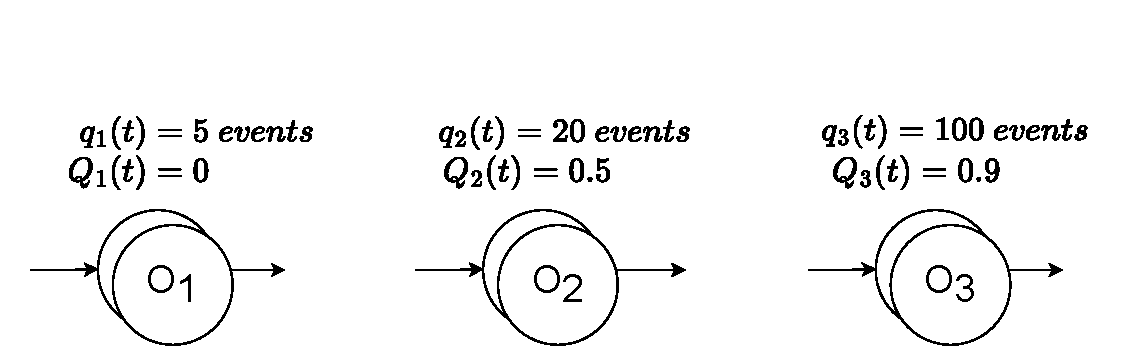
\includegraphics[width=0.8\textwidth]{figures/concepts/RA-SPS-Metric-Q.pdf}
    \caption{Example of the \textit{Queue} metric.}
    \label{fig:rsps-metric-q}
\end{figure}

To determine the overall state of an operator, the \textit{State} metric, denoted $\delta_i(t)$, is defined by Equation \ref{eq:rsps-delta}. It uses the previously defined metrics $U_i(t)$, $Q_i(t)$, and $E_i(t)$. By introducing weights ($\omega_U$, $\omega_Q$, and $\omega_E$), the impact of the 3 metrics can be balanced, allowing, therefore, the study of the relevance of each metric in different load scenarios.

\begin{equation}
    \delta_i(t) = U_i(t) \times \omega_U + Q_i(t) \times \omega_Q + E_i(t) \times \omega_E
    \label{eq:rsps-delta}
\end{equation}

The $\delta_i(t)$ value characterizes the overall state of an operator as shown in Figure \ref{fig:rsps-metric-state}. Following a threshold-based approach, two bounds are defined: the upper bound $\delta_{u}$ and the lower bound $\delta_{l}$. Considering these bounds, an operator can be in one of the three following states: \textit{overloaded}, \textit{stable}, or \textit{underloaded}. These states give information about an operator's \textit{effectiveness} and \textit{efficiency}. \textit{Effectiveness} is the capacity to fully process the input data, while \textit{efficiency} is the capacity to process data by taking advantage of the available resources. If an operator is \textit{overloaded}, it is not capable of processing all the input data, losing efficiency. On the other hand, if the operator is \textit{underloaded}, it processes the input data effectively but not efficiently. Finally, an operator whose state is \textit{stable} processes input data both efficiently and effectively.

\begin{figure}[!ht]
    \centering
    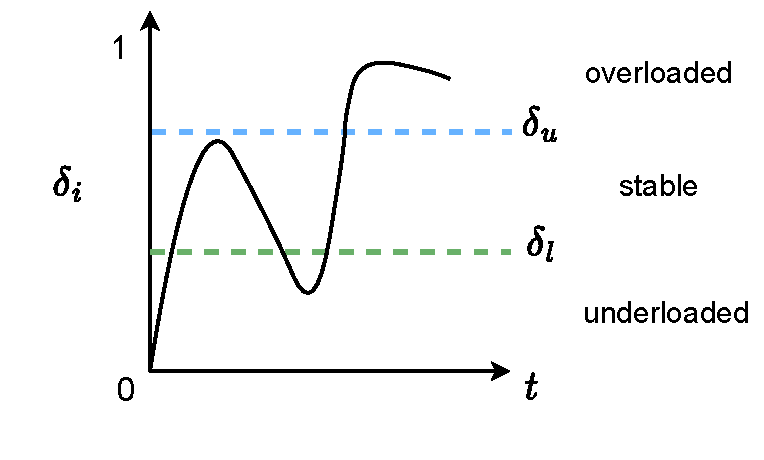
\includegraphics[width=0.5\textwidth]{figures/concepts/RA-SPS-Metric-Delta.pdf}
    \caption{Example of the evolution of the \textit{State} metric in the operator $O_i$.}
    \label{fig:rsps-metric-state}
\end{figure}

\subsection{MAPE implementation}
Monitoring, Analysis, Planning, and Execution compose the MAPE control loop. This model is exploited in most autonomic systems. By repeating these four steps, the system can detect issues by analysing data. If a problem is found, a strategy is developed and the executed to solve the issue. The MAPE control loop brings the system autonomic features such as self-configuration and self-optimization. Figure \ref{fig:rsps-mape} presents the
architecture of \rSPS{}:

\begin{figure}[!ht]
    \centering
    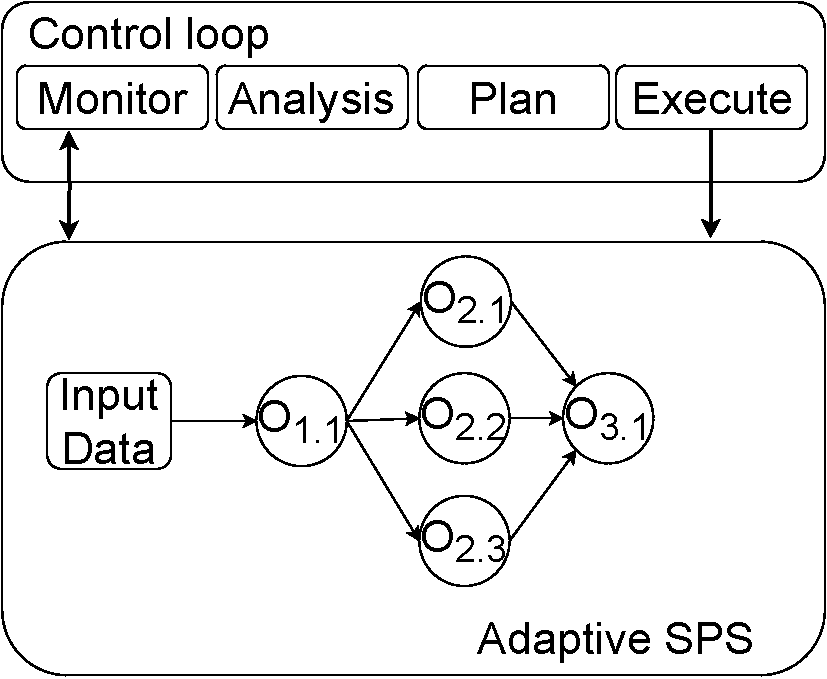
\includegraphics[width=0.45\textwidth]{figures/concepts/RA-SPS-Architecture.pdf}
    \caption{The architecture of \rSPS{}.}
    \label{fig:rsps-mape}
\end{figure}

In our system, the MAPE model integrates the before-mentioned components where each of the four MAPE modules performs the following tasks: 
\begin{enumerate} 
    \item \textit{Monitor}: module in charge of collecting statistics from the DAG. At a predefined time interval $t$, the monitor requests the values of $\mu_i(t)$, $et_i(t)$, and the number of queued events $q_i$.
    \item \textit{Analysis}: The module analyses the metrics of each operator and determines its status according to Equation \ref{eq:rsps-delta}.    
    \item \textit{Plan}: Based on the previous analysis, the \textit{Plan} module defines whether it is necessary or not to modify the system resource capacity. See Algorithm \ref{alg:rsps-planning} presented in Section \ref{rsps-planning}.
    \item \textit{Execute}: module in charge of carrying out the change in an operator's current number of replicas, if required by the \textit{Plan} module.
\end{enumerate}

\subsection{Planning}
\label{rsps-planning}

Algorithm \ref{alg:rsps-planning} that presents the algorithm executed by the \textit{Plan} module for the $O_i$ operator, deciding if the number of replicas of $O_i$ should be increased (or decreased) by $k$ or remain the same.
It uses a fixed value for $k$ for the \rSPS{} evaluation (see Section \ref{exp:params}). However, it is possible to dynamically modify this variable for the adaptation of the SPS.

Therefore, the aim of the algorithm is to modify the number of replicas of an operator $O_i$. If the operator is overloaded in line 3 ($\delta_i(t) > \delta_u$) or underloaded in line 7 ($\delta_i(t) < \delta_l$), the number of replicas should be increased or decreased respectively by $k$ replicas. Otherwise, if the operator state is stable, the number of replicas will not change. In order to ensure system stability, we define that an operator must remain in the same state by at least two consecutive time windows in line 2 ($\delta_i(t) = \delta_i(t-1)$) before carrying out any change in the number of replicas.

While the size of the pool of replicas is defined by the amount of cores, in case there is an overload of physical resources (VMs or nodes), it is necessary to limit the number of active replicas. For this, we determine a threshold $\delta_{E}$ for the metric $E_i(t)$, because the value of $E_i(t)$ indicates the degradation of the processing of the operator $O_i$. If $E_i(t)$ is greater than the threshold $\delta_{E}$ (line 4), the planning cannot increase the number of active replicas. In this way, we avoid an overload on the physical resources of the system and performance degradation of the SPS.

\begin{algorithm}[!ht]
 \caption{Adaptive planning algorithm according to the reactive approach for the operator $O_i$.}
 \begin{algorithmic}[1]
 	\REQUIRE Statistics Operator $O_i$ in time interval $t$.
 	\ENSURE Modifying the current number of active replicas of operator $O_i$.
	\STATE $\delta_i(t)$ $\gets$ calculateMultiMetric($U_i(t)$ , $Q_i(t)$ , $E_i(t)$)
	\IF {$\delta_i(t) = \delta_i(t-1)_i$}
		\IF {$\delta_i(t) > \delta_{u}$}
			\IF {$E_i(t) > \delta_{E}$}
				\STATE Add $k$ active replicas for $O_i$
			\ENDIF 
		\ELSIF {$\delta_i < \delta_{l}$}
			\STATE Remove $k$ active replicas for $O_i$
		\ENDIF
	\ENDIF
\end{algorithmic}
\label{alg:rsps-planning}
\end{algorithm}
\section{Predictive approach}
\label{predictive-approach}
Under highly variable input rate environments, input prediction is crucial in order to adapt the system processing logic over the time, which will keep events flowing, ensuring accurate results.

In our second proposal, denoted  \pSPS{}, we use a prediction model for the estimation of the optimal number of replicas for a given operator in the DAG. Therefore, unlike \rSPS{}, a reactive approach that focuses on detecting traffic peaks, \pSPS{}, a predictive approach, focuses on finding patterns in the traffic, predicting possible overloads or underloads.

Table~\ref{tab:notations} summarizes all the parameter's notations used in \pSPS{}. 

\begin{table}[!ht]
\begin{tabular}{|c|l|}
    \hline
    \textit{\textbf{Parameter}}     & \textit{\textbf{Description}}             \\  \hline
    $O_i$                           & operator $i$ \\
    $t$                             & time interval number \\ 
    $td$                            & time interval duration  \\
    $et_i$                          & average execution time of one event by $O_i$  \\
    $q_i(t)$                        & queue of events received and not processed by $O_i$ at the end of $t$ \\
    $\lambda_G(t)$                  & number of events sent by input data during $t$ \\
    $\lambda^r_i(t)$                & number of events received by $O_i$ during $t$\\
    $\lambda^p_i(t)$                & number of events received by $O_i$ sent from $O_p$ during $t$\\
    $\mu_i(t)$                      & number of events processed by $O_i$ during $t$\\
    $\theta_x(t)$                   & percentage of events processed of $\lambda_G(t)$ by $O_x$ during $t$\\
    $O_i^p$                         & predecessor operator of $O_i$ in the SPS DAG \\
    $\theta_i^p(t)$                 & percentage of events produced by $O_i^p$ sent to $O_i$ during $t$\\
    $\widehat{\lambda_G}(t+1)$      & predicted number of events sent by input data during $t+1$ \\
    $\widehat{\lambda_i}(t+1)$      & predicted number of events to process by $O_i$ during $t+1$ \\
    $\widehat{\lambda_i^r}(t+1)$    & predicted number of events received by $O_i$ during $t+1$ \\
    $\widehat{\lambda_i^q}(t+1)$    & predicted number of queued events to  be processed by $O_i$ during $t+1$ \\
    $r_i(t+1)$                      & number of replicas of $O_i$ computed at the end of $t$  \\
    \hline
\end{tabular}
\caption{Parameters notation and their description in \pSPS{}.}
\label{tab:notations}
\end{table}

\subsection{Predictive model}
% REPLICAS
The aim of our predictive model is to estimate how many active replicas would be necessary for operator $O_i$ to process the number of input events for the next time interval $t+1$ ($\widehat{\lambda_i}(t+1)$). It considers the processing capacity of $O_i$ as the average execution time of one event at the operator ($et_i$). At the end of each interval, the number of replicas is calculated following Equation \ref{eq:prediction-replicas}.

\begin{equation}
    \label{eq:prediction-replicas}
    r_i(t+1) = \frac{\widehat{\lambda_i}(t+1) \times et_i}{td}\\
\end{equation}

Let us consider that the time interval duration ($td$) equals $1000~ms$. Figure \ref{fig:prediction-replicas} shows an example composed by three independent operators  ($O_1$, $O_2$, and $O_3$) which have different average execution time of one event ($et_i$).  At the beginning of $t$, all the three operators have two replicas ($r_i = 2$). And by prediction, they will receive the same number of events $\widehat{\lambda_i}(t+1)$. 

In this example, due to $et_i$'s differences, Equation \ref{eq:prediction-replicas} will render $r_1(t+1)=2$, $r_2(t+1)=1$, and $r_3(t+1)=4$ at the end of $t$. Such results inform that the number of $O_1$'s active replicas should not change but that of $O_2$ (resp., $O_3$) is overestimated (resp., underestimated) and should be reduced (resp., increased) to one (resp., four). 

\begin{figure}[!ht]
    \centering
    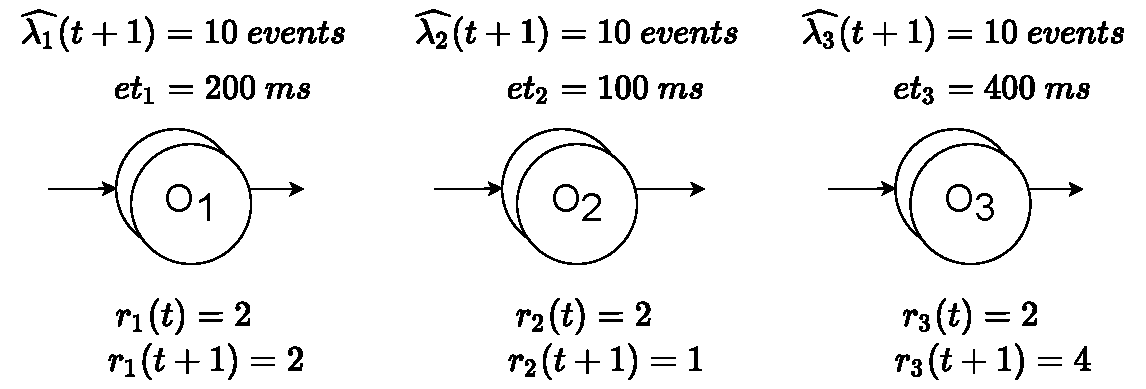
\includegraphics[width=0.9\textwidth]{figures/concepts/PA-SPS-PredictiveModel.pdf}
    \caption{Example of the number of replicas calculation, according Equation \ref{eq:prediction-replicas}.}
    \label{fig:prediction-replicas}
\end{figure}

We point out that since prediction of a number of active replicas depends on multiple factors, dynamically determining it is not trivial.
Thus, we model this complex problem so that the value of $\widehat{\lambda_i}(t+1)$ is determined by Equation \ref{eq:prediction-lambda} which, in turn, is determined by the prediction of received events ($\widehat{\lambda_i^r}(t+1)$) and the prediction of queued events ($\widehat{\lambda_i^q}(t+1)$) during the next time interval.

\begin{equation}
\label{eq:prediction-lambda}
    \widehat{\lambda_i}(t+1) = \widehat{\lambda_i^r}(t+1) + \widehat{\lambda_i^q}(t+1)
\end{equation}

% DEPENDECY (Domino Effect)
In most SPS, the processing logic is represented by a DAG. The latter establishes a dependency condition where operators share a stream of events according to their location in the DAG. For example, let's consider a linear DAG with two operators (see Figure \ref{fig:sps-dependence}), $O_1$ and $O_2$, and their respective values of $\lambda^r_i(t)$ and $\mu_i(t)$ (see Table \ref{tab:notations}). $\mu_1(t)$ and $\lambda^r_2(t)$ are equal since operator $O_1$ has sent all the events it has processed to its single successor $O_2$. If $i$ is the initial single DAG operator, then $\lambda^r_i(t)$ equals $\lambda_G(t)$ ($\lambda^r_1(t) = \lambda_G(t)$).

Note that the increase of $O_p$'s number of active replicas at the end of the interval $t$ has a direct impact in $O_p$'s successors, since, in this case, $\mu_p(t+1)$ increases and thus,  $\lambda^r_i(t+1)$ too, inducing a domino effect that the prediction formulations should avoid. For example, in Figure \ref{fig:sps-dependence}, if $\mu_1(t+1)$ increased from $5$ to $10$ events, due to the replication of $O_1$ at the end of $t$, $\lambda^r_2(t+1)$ would increase as well. Hence, if the operators process all received events during $t+1$, we have that $\lambda_G(t+1)=\lambda^r_1(t+1)=\mu_1(t+1)=\lambda^r_2(t+1)$ and, consequently, all operators $O_i$ are dependent on $\lambda_G(t)$. 

\begin{figure}[!ht]
    \centering
    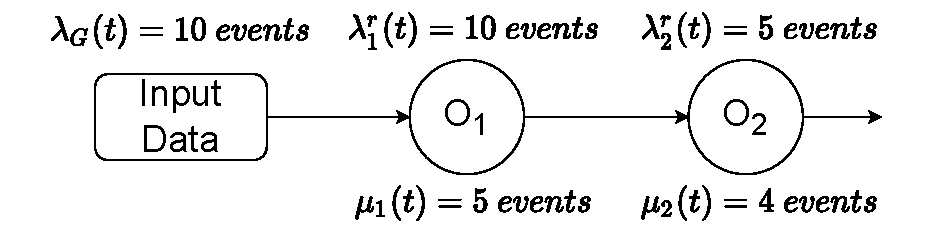
\includegraphics[width=0.8\textwidth]{figures/concepts/PA-SPS-Dependence.pdf}
    \caption{DAG operators dependence example.}
    \label{fig:sps-dependence}
\end{figure}


% PREDICTION INPUT
The above example is a borderline case. In a SPS DAG, not always, all the output processed events of $O_i^p$, the predecessor operator of $O_i$, will be sent to $O_i$. It might happen that $O_i^p$ splits, filters, or replicates the events into several streams, sending each of them to one of its different successor operators in the DAG. Thus, we define Equation \ref{eq:theta-predecessor}, where $\theta_i^p$ parameter tackles this issue by informing the percentage of processed events of $O_i^p$ sent to $O_i$.

\begin{equation}
  \label{eq:theta-predecessor}
  \theta_i^p(t) =  \frac{\lambda^p_i(t)}{\mu_p(t)}\\
\end{equation}

% THETA
Considering the condition of dependence among the operators, $\theta_{i}(t)$ is defined as the sum of the events processed by the predecessors of $O_i$, where it is determined by all the predecessor operators $O^p_i$ as presented in Equation \ref{eq:theta}. Note that $\theta_i(t)$ must be calculated from the initial operators.

\begin{equation}
  \label{eq:theta}
  \theta_i(t) =  \sum_{p \in pred(O_i)} \theta_i^p(t) \times \theta_p(t)\\
\end{equation}

Thus, we define Equation \ref{eq:prediction-input}, which predicts the number of events received by the operator $O_i$ during $t+1$. For its calculation, the percentage of events processed by operator $O_i$ is used ($\theta_i(t)$), according to the prediction of the number of events sent by the input data ($\widehat{\lambda_G}(t+1)$). Note that a predictive model is used to calculate $\widehat{\lambda_G}(t+1)$ (see Section \ref{psps-input-prediction}).

\begin{equation}
    \label{eq:prediction-input}
  \widehat{\lambda_i^r}(t+1) =  \widehat{\lambda_G}(t+1) \times \theta_i(t)\\
\end{equation}

Figure \ref{fig:prediction-input} shows a DAG example and $\theta_i^p$ value which was  estimated applying Equation \ref{eq:theta-predecessor}. It is worth pointing out that, given the dependence among the operators, it is necessary to start from the initial operator downstream to the last one. Since $\theta_1$ is equal to $1$, $O_1$ receives all the events sent from the input and then splits them among $O_2$ and $O_3$.  In this case, the two operators do not receive all the events from their respective predecessor, $O_1$; therefore $\theta_2$ and $\theta_3$ have values $0.7$ and $0.3$ respectively. Finally, operator $O_4$ receives events from its predecessor operators $O_2$ and $O_3$. However, $O_2$ does not send all its processed events to $O_4$, but only $\theta_4^2=0.4$, unlike $O_3$ which sends all processed events to $O_4$ ($\theta_4^2=1$). The value of $\theta_4$ is, therefore, $0.58$, according to Equation \ref{eq:theta}. 

\begin{figure}[!ht]
    \centering
    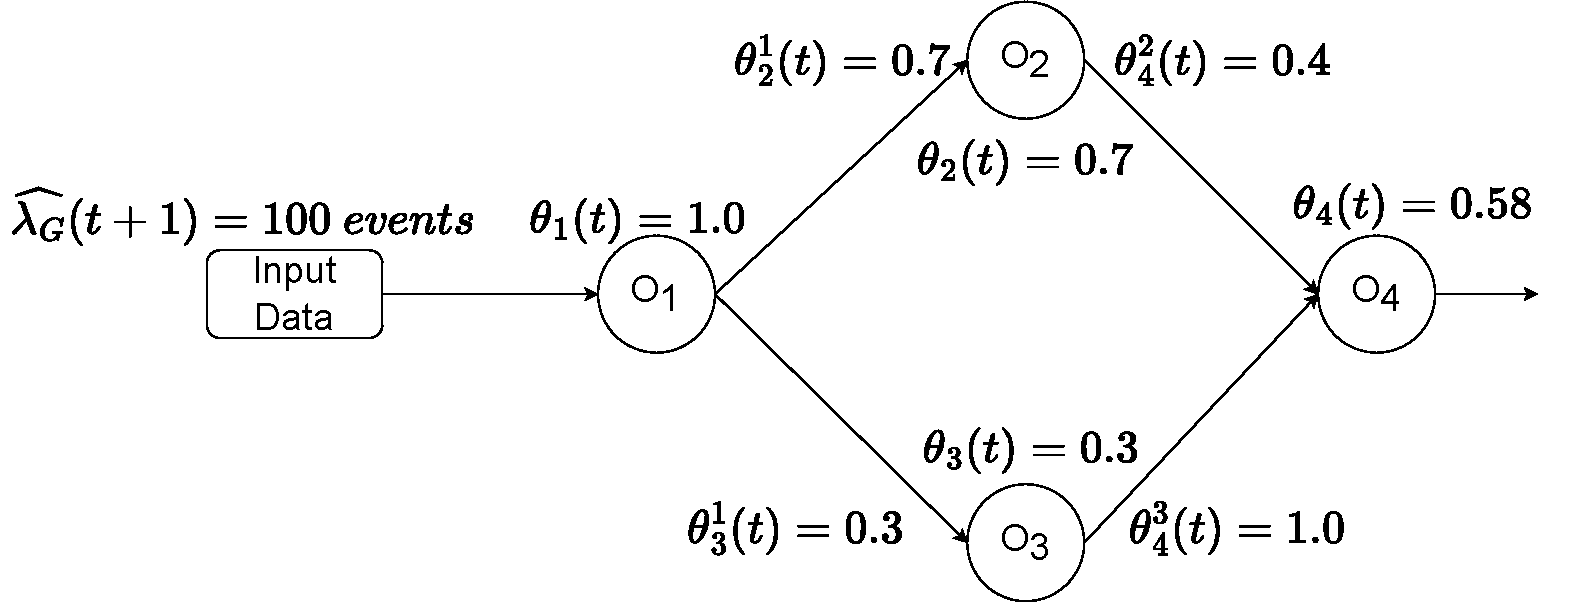
\includegraphics[width=1\textwidth]{figures/concepts/PA-SPS-PredictionInput.pdf}

    \vspace*{0.5cm}
    
    \begin{tabular}{c|c|c|c|c}
        & $O_1$ & $O_2$ & $O_3$ & $O_4$\\ \hline
        $\widehat{\lambda^r_i}(t+1)$ & 100 & 70 & 30 & 58
    \end{tabular}
    \caption{DAG example of predicted received number of events according to Equation \ref{eq:prediction-input}.}
    \label{fig:prediction-input}
\end{figure}

% QUEUE

Finally, we should consider the events received and not processed during $t$ by $O_i$ which are kept in $q_i(t)$. Hence, the number of input events $\widehat{\lambda_i}(t+1)$ that $O_i$ should actually process in $t$ is composed not only of received events $\widehat{\lambda_i^r}(t+1)$ but also of the events queued in $O_i$ and its predecessor operators $O^i_p$ because of the domino effect on the DAG.

For this reason, Equation \ref{eq:prediction-queue} is defined, where $\widehat{\lambda_i^q}(t+1)$ consists of the number of events queued in $O_i$ and the percentage of queued events that will be sent by its predecessor operators $O^p_i$ during $t+1$. Note that there is one queue per operator.

\begin{equation}
\label{eq:prediction-queue}
  \widehat{\lambda_i^q}(t+1) =  |q_i(t)| + \sum_{p \in pred(O_i)} \widehat{\lambda_p^q}(t+1) \times \theta_p(t)
\end{equation}


% INPUT PREDICTION
\subsection{Input prediction}
\label{psps-input-prediction}
As mentioned above, Equation \ref{eq:prediction-input} used $\widehat{\lambda_G}(t+1)$, which indicates the predicted number of events sent by the input data during $t+1$. Its prediction is based on the previous observation windows according to a number of samples $s$. The observation time interval is determined by $to$. The prediction is applied by one of the following models:

\begin{itemize}
    \item \textit{Basic}: considers that the input data values during $t+1$ will behave the same way as they did during $t$.
    \item \textit{LR}: uses a simple linear regression similar to the one presented in \citep{montgomery2021introduction}.
    \item \textit{FFT}: Fast Fourier Transform decomposes functions depending on space or time into functions depending on frequency. It allows to predict the input data by modeling its behavior as a time series \citep{nussbaumer1982fast}.
    \item \textit{ANN}: uses a neural network regression model, specifically a Multi-Layer Perceptron (MLP). It implements an MLP algorithm for training and testing data sets using backpropagation and stochastic gradient descent methods \citep{riedmiller2014multi}. The parameters values used in this model where extracted from \citep{PedregosaVGMTGBPWDVPCBPD11}.
    \item \textit{RF}: Random Forest combines learning methods with the decision tree framework to create multiple randomly drawn decision trees from the data. \citep{rigatti2017random}. The parameters used are the values for defects in \citep{PedregosaVGMTGBPWDVPCBPD11}.
\end{itemize}


\subsection{MAPE implementation}
As with the reactive approach, in \pSPS{} we will use the MAPE model for the automation of system adaptation. The big difference is in the \textit{Analysis} module, because it performs a request to the predictor model for input rate prediction. Figure \ref{fig:psps-mape} presents the
architecture of \pSPS{}:

\begin{figure}[!ht]
    \centering
    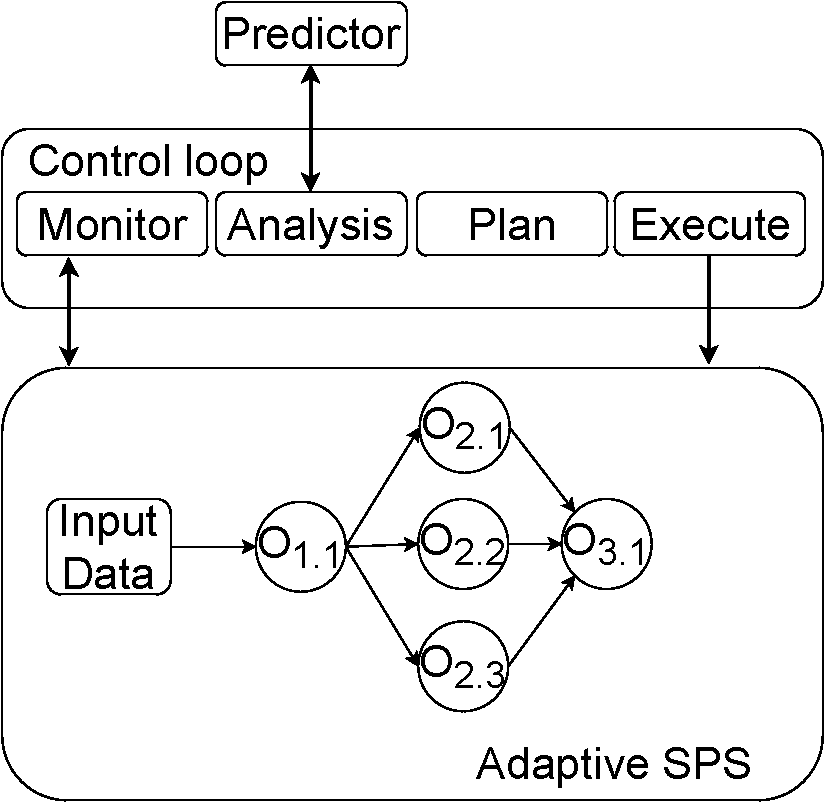
\includegraphics[width=0.45\textwidth]{figures/concepts/PA-SPS-Architecture.pdf}
    \caption{The architecture of \pSPS{}.}
    \label{fig:psps-mape}
\end{figure}

In our system, the MAPE model integrates the before-mentioned components where each of the four MAPE modules performs the following tasks: 
\begin{enumerate} 
    \item \textit{Monitor}: Module in charge of collecting statistics from the DAG. At a predefined time interval $t$, the monitor requests the values of $\lambda_i(t)$, $et_i$, and the number of queued events $q_i(t)$.
    \item \textit{Analysis}: The module analyses input data and predicts its behaviour following Equation \ref{eq:prediction-lambda}. Note that the analysis is performed for each operator in the DAG.
    \item \textit{Plan}: Based on the previous analysis, the \textit{Plan} module defines whether it is necessary or not to modify the system resource capacity. For this, we define Algorithm \ref{alg:psps-planning} which is explained in Section \ref{psps-planning}.  
    \item \textit{Execute}: Module in charge of carrying out the change in an operator's current number of replicas, if required by the \textit{Plan} module.
\end{enumerate}


\subsection{Planning}
\label{psps-planning}
Algorithm \ref{alg:psps-planning} presents the algorithm executed by the \textit{Plan} module for the $O_i$ operator, deciding if the number of replicas of $O_i$ should be increased (or decreased) by $k$ or remain the same.

First, the algorithm determines the number of replicas for the next time interval is computed (line 1). To this end, the number of necessary replicas is calculated according to Equation \ref{eq:prediction-replicas}, using an input data predictor to determine the future behaviour of the input stream. Then, the $getReplicas(O_i)$ function returns the current active replicas of $O_i$. Hence, the difference between the prediction and the current number of replicas will be the number of replicas ($k_i$) to be modified (line 2). If the value of $k$ is positive, then $k_i$ replicas are activated (line 4). If the value of $k$ is negative, then $k_i$ replicas are deactivated (line 6). If the value of $k$ is 0, then the same number of active replicas is kept.

\begin{algorithm}[!ht]
\caption{Adaptive planning algorithm according to the predictive approach for the operator $O_i$.}
 \begin{algorithmic}[1]
 	\REQUIRE Statistics Operator $O_i$ in time interval $t$.
 	\ENSURE Modifying the current number of active replicas of operator $O_i$.
	\STATE $r_i(t+1) \gets$ computeReplicas($\widehat{\lambda_i}(t+1)$ , $et_i$, $td$)
	\STATE $k_i \gets r_i(t+1)$ - getReplicas($O_i$)
	\IF {$k_i > 0$}
		\STATE Add $k_i$ active replicas to $O_i$
	\ELSIF {$k_i < 0$}
		\STATE Remove $k_i$ active replicas from $O_i$
	\ENDIF
\end{algorithmic}
\label{alg:psps-planning}
\end{algorithm}
\section{Conclusion}
In this section we propose two adaptive SPSs, \rSPS{} and \pSPS{}, under a reactive and predictive approach respectively. These adaptive SPSs dynamically modify the number of operator replicas based traffic fluctuations. Both proposals are implemented on top of \textit{Storm}.

Moreover, two other features were included in the two adaptive SPSs. The first consists of a \textit{pool of replicas} aiming at avoiding the restart the SPS when the number of active replicas is modified. The second consists of a grouping strategy, which denoted \textit{Load-Aware} grouping. The latter determines which replica will process the event according to the load of the operator's active replicas, the latter the load balance among the replicas.

The first adaptive presented SPS is \rSPS{}, which is based on a reactive approach. Its aim is to adapt resources according to the analysis of traffic peaks in short periods of time. For this propose, the multi-metric $\delta_i(t)$, called \textit{State} metric is used to define the state of a given operator: overloaded, stable or underloaded. Each state indicates the behaviour of each operator, so that the Planning Algorithm can determine if any modification is necessary. The \textit{State} metric is defined by three weighted metrics: $U_i(t)$ that determines the percentage utilisation of $O_i$ during interval $t$; $E_i(t)$ that determines the processing degradation of the $O_i$ operator during interval $t$; $Q_i(t)$ that determines the impact of queue size on the $O_i$ operator during interval $t$.

The second adaptive presented SPS is \pSPS{}, which is based on a predictive approach. It aims to find patterns in the traffic to predict possible overloads or underloads in the SPS. To this end, the number of replications needed by operator $O_i$ during the next time interval $t+1$, denoted $r_i(t+1)$, is predicted. This value is defined by the average execution time of an event by operator $O_i$ and the predicted number of events received by operator $O_i$ during the next time interval $t+1$. To predict the number of events received by operator $O_i$, the predicted number of events sent by the input data and the number of queued events are considered. Furthermore, the prediction also considers the dependency among operators, in order to mitigate a possible cascade effect due to the change of the number of replicas. For the prediction of events sent by the input data, the use of a predictive model based on mathematical model or artificial intelligence model is proposed.

\chapter{Experimentation}
\label{experimentation}
The goal of this chapter is to evaluate our adaptive SPS, both the reactive and predictive approaches. In this way, we will analyze the impact of adaptation on the performance of the SPS. %For comparison, there will be three sections: adaptive SPS, \rSPS{} and \pSPS{}.

Section \ref{exp:scenario} presents the experimental scenario, specifying the environment, the dataset, the parameters and the evaluation metrics. Section \ref{exp:modified-sps} presents the evaluation of our extended version our extended version of Storm, which uses a replica pool and \textit{Load-aware} grouping. Section \ref{exp:reactive} presents the evaluation and analysis of \rSPS{}, using different configurations in their weights and applications. Finally, Section \ref{exp:predictive} presents the evaluation and analysis of \pSPS{}, both of the parametrization used as well as a comparison with other existing adaptive SPS.

\section{Experiment scenario}
\label{exp:scenario}
In this section, we describe the components necessary for the creation of an experiment scenario, which has three components: environment, dataset and application. For each experiment, we considered a set of measures for which the difference in behaviour was negligible.

Section \ref{exp:enviroment} presents the environment that is the architecture used for the deployment of the adaptive SPS. Section \ref{exp:dataset} presents the dataset refers to the traffic used to provide an input data stream. Section \ref{exp:app} presents the applications designed with its respective processing according to the DAG and the type of data used. Section \ref{exp:params} presents the parameters used by the adaptive SPSs. Finally, Section \ref{exp:metric} presents the evaluation metrics.
 
\subsection{Environment} 
\label{exp:enviroment}
All the experiments were conducted on the Google Cloud Platform (GCP) using seven Virtual Machines (VMs): three in charge of Zookeeper, seven as Supervisor nodes, and one for running both the Nimbus and the adaptive SPS. Our test environment is presented in Figure \ref{fig:exp-testbed}. 

Three types of machines were used: a \texttt{n1-standard-1} (1 CPU, 2.2 GHz, 3.75 GB of RAM) machine for hosting Zookeeper VMs, a \texttt{n1-standard-4} (4 CPU, 2.2 GHz, 15 GB of RAM) for Nimbus and the adaptive SPS, and a \texttt{n1-highcpu-8} (8 CPU, 2.2GHz, 7.2GB of RAM) machine for the Supervisors VMs.

\begin{figure}[!ht]
      \centering
     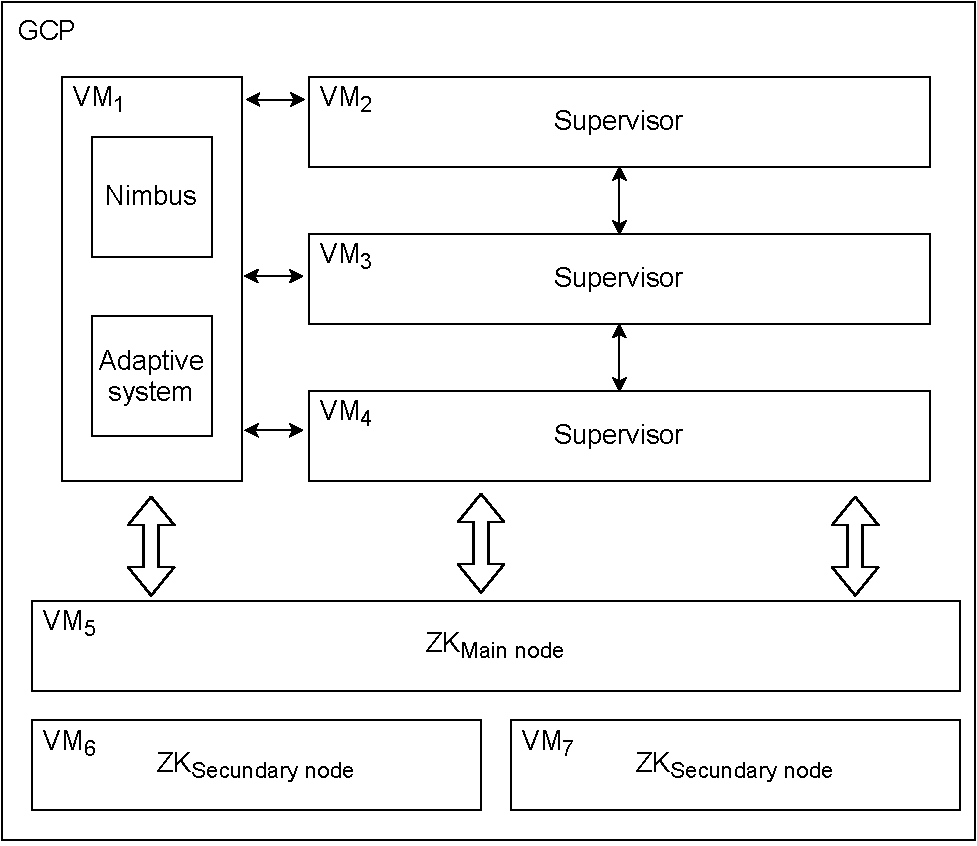
\includegraphics[width=0.65\textwidth]{figures/exp/GCP.pdf}
     \caption{Development environment on GCP.}
     \label{fig:exp-testbed}
\end{figure} 
 
\subsection{Dataset}
\label{exp:dataset}
We have considered four dataset for the experiments: \textit{Twitter Gaussian}, \textit{Twitter Smoothed}, \textit{Twitter Raw}, \textit{Logs} and \textit{DNS}.

\begin{itemize}
\item \textit{Twitter Gaussian}: This dataset is traffic that follows a Gaussian distribution, whose data are tweets related to COVID-19 \cite{PXF2CU2020}. Figure \ref{fig:exp-dataset-twitter-gaussian} shows the traffic provided by this distribution.

\begin{figure}[!ht]
\centering
    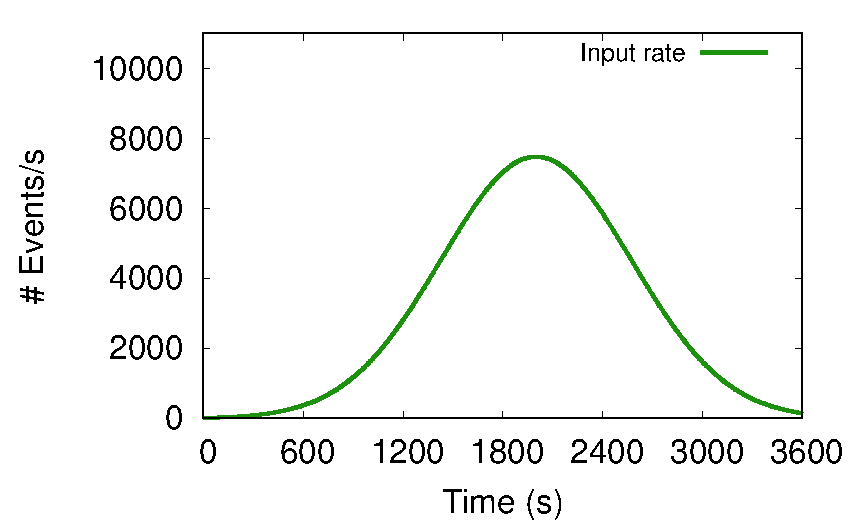
\includegraphics[width=0.5\textwidth]{figures/exp/Dataset-TwitterGaussian.pdf}
    \caption{Traffic shape of Twitter Gaussian dataset.}
    \label{fig:exp-dataset-twitter-gaussian}
\end{figure}

\item \textit{Twitter Raw}: This dataset is based on data from Twitter related to COVID-19, with 237 million tweets \cite{PXF2CU2020}. Figure \ref{fig:exp-dataset-twitter-raw} shows the traffic provided by this dataset.

\begin{figure}[!ht]
\centering
    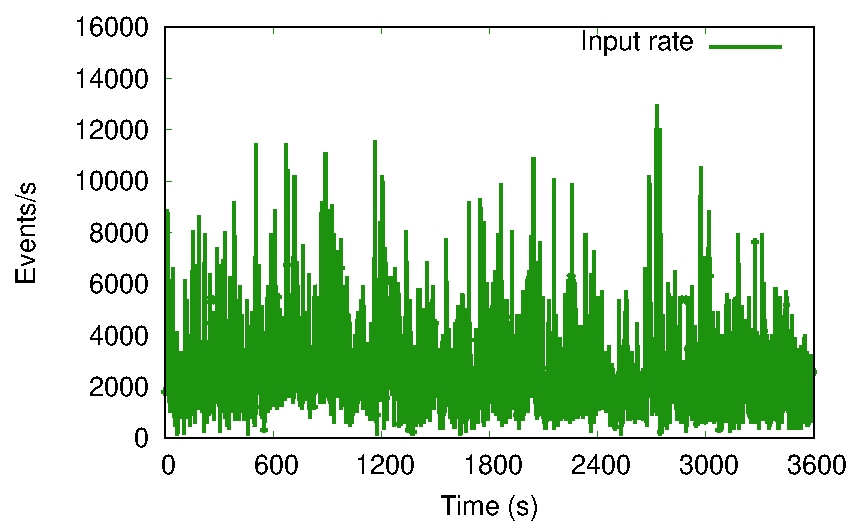
\includegraphics[width=0.5\textwidth]{figures/exp/Dataset-TwitterRaw.pdf}
    \caption{Traffic shape of Twitter Raw dataset.}
    \label{fig:exp-dataset-twitter-raw}
\end{figure}

\item \textit{Twitter Smoothed}: This dataset is based on \textit{Twitter Raw}. However, we have considered only a sample of these tweets in the experiments, i.e., those in periods of the datasets that present high rate variation. In other words, we select a combination of traffic spikes and under spikes to compose the input traffic for the experiments. The methodology adopted to build the testing dataset was introduced in \cite{BodikFFJP10}. Figure \ref{fig:exp-dataset-twitter-raw} represented the traffic designed \ref{fig:exp-dataset-twitter-smoothed}.

\begin{figure}[!ht]
\centering
    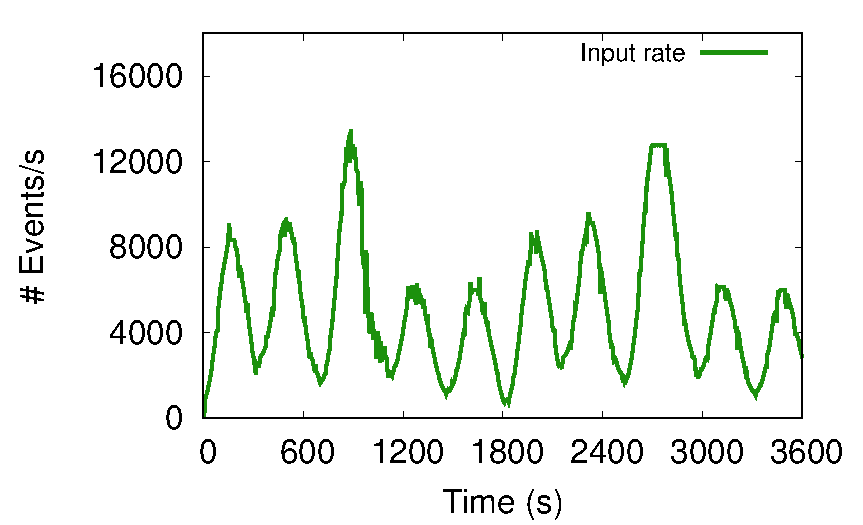
\includegraphics[width=0.5\textwidth]{figures/exp/Dataset-TwitterSmoothed.pdf}
    \caption{Traffic shape of Twitter Smoothed dataset.}
    \label{fig:exp-dataset-twitter-smoothed}
\end{figure}

\end{itemize}

\begin{itemize}
\item \textit{DNS}:  This dataset is based on network traffic, which was created to test DNS over HTTPS, a more secure version of the DNS protocol \citep{MontazeriShatoori20}. We used the same methodology mentioned above was used to build the dataset. Figure \ref{fig:exp-dataset-dns} shows the log traffic provided by this dataset.
\end{itemize}

\begin{figure}[!ht]
\centering
    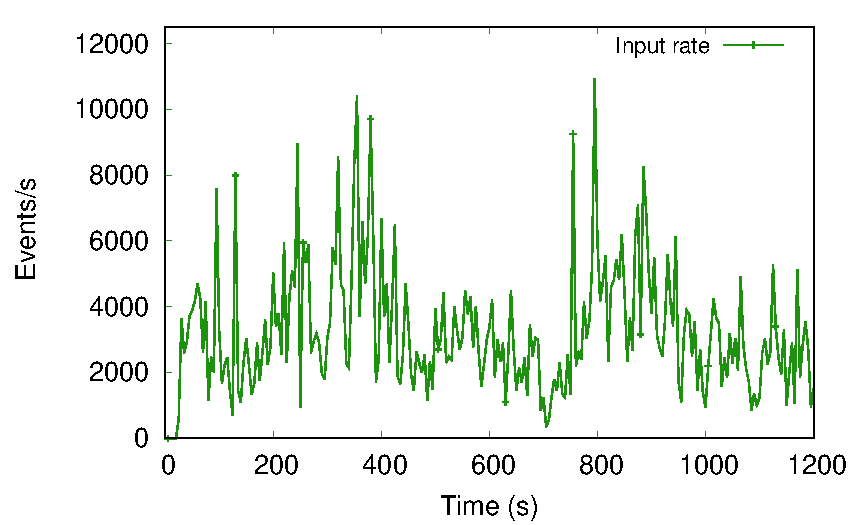
\includegraphics[width=0.5\textwidth]{figures/exp/Dataset-DNS.pdf}
    \caption{Traffic shape of DNS dataset.}
    \label{fig:exp-dataset-dns}
\end{figure}

\begin{itemize}
\item \textit{Log}: This dataset is based on system logs from a distributed system  \citep{LogsPaper}. We used the same methodology mentioned above was used to build the dataset. Figure \ref{fig:exp-dataset-log} shows the log traffic provided by this dataset.
\end{itemize}

\begin{figure}[!ht]
\centering
    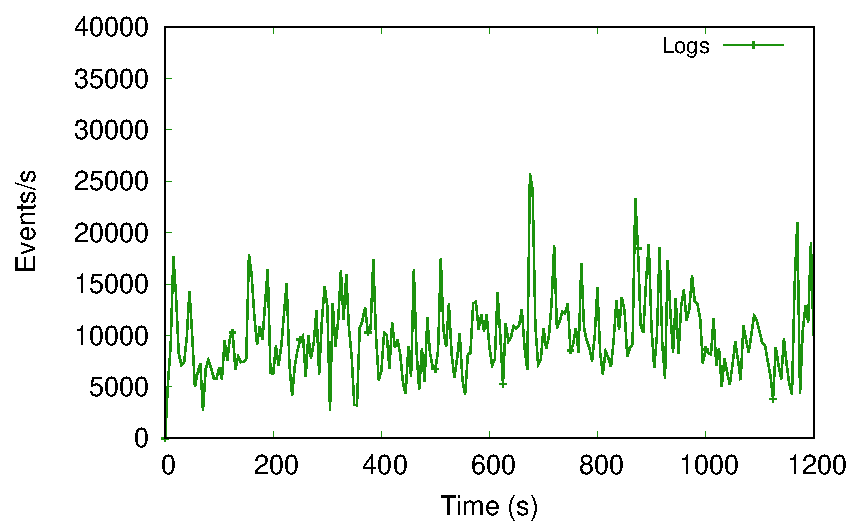
\includegraphics[width=0.5\textwidth]{figures/exp/Dataset-Logs.pdf}
    \caption{Traffic shape of Log system dataset.}
    \label{fig:exp-dataset-log}
\end{figure}

\subsection{Application}
\label{exp:app}
For each traffic, we have at least one application to be used. The applications designed for the experimental phase are listed below:

\begin{itemize}
\item \textit{Twitter linear}: It is a linear DAG for \textit{Twitter} dataset, which is composed of four operators.

\begin{itemize}
	\item \textit{Detection}: Its goal is to detect tweet events of a Twitter data streaming according to a topic, subtopic, category, and subcategory list of keywords. Each operator has one of these lists and verifies if any of the words of a tweet is included in the list in question. Therefore, in the sequence, the first, second, third, and fourth operators respectively determine the topic, subtopic, category, and subcategory of each tweet as shown in Figure \ref{fig:app-twitter-linear-1}.
	
\begin{figure}[!ht]
\centering
    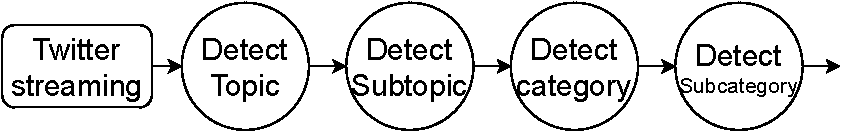
\includegraphics[width=0.65\textwidth]{figures/exp/App-Twitter-Linear-1.pdf}
    \caption{Detection Twitter application in SPS.}
    \label{fig:app-twitter-linear-1}
\end{figure}	
	
	\item \textit{Classification}: Its goal is to classify tweet events of a Twitter data streaming. The first classifier determines whether the text is positive, negative or neutral, and the second identifies the person who has published them. Classified tweets are stored in a database. Figure \ref{fig:app-twitter-linear-2} shows this application.
\begin{figure}[!ht]
\centering
    \includegraphics[width=0.65\textwidth]{figures/exp/App-Twitter-Linear-2.pdf}
    \caption{Classification Twitter application in SPS.}
    \label{fig:app-twitter-linear-2}
\end{figure}			
\end{itemize}

\item \textit{Twitter complex}: It is a complex DAG for \textit{Twitter} dataset, which is composed of eight operators. Figure \ref{fig:app-twitter-complex} shows the DAG of this application. It analyses Twitter streaming containing information such as news or opinions. Depending on the type of information, the stream can be split. Finally, results are stored in a database.

\begin{figure}[!ht]
\centering
    \includegraphics[width=0.75\textwidth]{figures/exp/App-Twitter-Complex.pdf}
    \caption{Classification Twitter application in SPS.}
    \label{fig:app-twitter-complex}
\end{figure}

\item \textit{Log}: It is a linear DAG for \textit{Log} dataset, which is composed of four operators. Figure \ref{fig:app-log} shows its representation of DAG. Its objective is to determine the importance of the log trace.

\begin{figure}[!ht]
\centering
    \includegraphics[width=0.65\textwidth]{figures/exp/App-Log.pdf}
    \caption{Log application in SPS.}
    \label{fig:app-log}
\end{figure}

\item \textit{DNS}: It is a linear DAG for \textit{DNS} dataset, which is composed of four operators. Figure \ref{fig:app-dns} shows its representation of DAG. Its goal is analyses and classifies events based on DNS traffic.

\begin{figure}[!ht]
\centering
    \includegraphics[width=0.65\textwidth]{figures/exp/App-DNS.pdf}
    \caption{DNS application in SPS.}
    \label{fig:app-dns}
\end{figure}

\end{itemize}

\subsection{Parameters}
\label{exp:params}
Table \ref{tab:exp-reactive-parameters} summarizes \rSPS{} parameters and their respective values. These values were determined according to expertise and learning outcomes obtained from the results of several previous experiments using different parametrizations.

\begin{table}[!ht]
\centering
\begin{tabular}{|c|l|c|}
\hline
Parameter     & Description & Value
\\ \hline \hline
$td$          & Time interval duration & 25 sec  \\ \hline
$\delta_{u}$    & Operator state upper limit & 0.7     \\ \hline
$\delta_{l}$    & Operator state lower limit   & 0.3     \\ \hline
$\delta_{E}$    & Limit for adding replicas  & 0.7     \\ \hline
$\omega_U$    &  $U$ metric weight & 0.45    \\ \hline
$\omega_Q$    & $Q$ metric weight & 0.45    \\ \hline
$\omega_E$    & $E$ metric weight & 0.1     \\ \hline
$k$  		  & Number of active replicas to add/remove & 1       \\ \hline
\end{tabular}
\caption{\rSPS{} parameters and their values.}
\label{tab:exp-reactive-parameters}
\end{table}

Table \ref{tab:exp-predictive-parameters} summarizes \pSPS{} parameters and their respective values. To determine the values of predictive model parameters, the model has considered obtaining a representative sampling based on the methodology presented in \citep{winters2017practical}.

\begin{table}[!ht]
\centering
\begin{tabular}{|c|l|c|}
\hline
Parameter     & Description & Value
\\ \hline \hline
$td$   & Time interval duration    							    & 30 sec  \\ \hline
$to$   & Observation time interval duration for predictor model & 1 sec    \\ \hline
$s$    & Number samples for predictor model     				& 100  \\ \hline
\end{tabular}
\caption{\pSPS{} parameters and their values.}
\label{tab:exp-predictive-parameters}
\end{table}

For \textit{Storm} parameters, we used default values \footnote{http://github.com/apache/storm/blob/master/conf/defaults.yaml}, except timeout to detect the failure of an event, $t_{out}=30s$, and queue size, $q_{size}=100000$. 

\subsection{Metrics}
\label{exp:metric}
For the evaluation, we have defined six evaluation metrics.
\begin{itemize}
    \item \textit{Saved resources}: proposed in \cite{LombardiABQ18}, this metric expresses the proportion of resources (active replicas) saved with respect to a statically over-provisioned configuration.
    It is defined by  $1-\frac{r}{r_{over}}$, with $r$ the number of active replicas, and $r_{over}$ the overestimated number of replicas. $r_{over}$ is the number of replicas needed to process all the events during the highest input rate peak of the benchmark. Note that if the value of the metric is close to 1, a high number of resources has been saved.
    \item \textit{Throughput degradation}: this  metric, also described in \cite{LombardiABQ18}, aims at analyzing the behavior of the system in terms of throughput stability. It is defined by  $\frac{\left | input_{rate} - output_{rate} \right |}{input_{rate}}$.  If the metric value is close to 0, the system has a good stability. On the other hand, if it is close to 1, the system is not capable to process the input rate and the system is unstable.
    \item \textit{Latency}: is the average time taken by an event between the moment it enters and leaves the SPS (end-to-end latency). This metric is relevant since SPSs are supposed to deliver real-time processed events.
    \item \textit{Difference in the number of processed events}: is the difference between the total number of processed events and the total number of received events. It is an important metric since SPSs are used to process high volumes of data.
    \item \textit{Error estimation input}: is the mean absolute percentage error of the difference between the input rate and the predicted input rate during each interval.
    \item \textit{Error estimation replica}: is the mean absolute percentage error of the difference between the number of replicas needed to process all events and the number of predicted replicas during each interval.
\end{itemize}

\section{Impact of the new features}
\label{exp:modified-sps}

The aim of this section is to evaluate the modifications made to our SPS, being an extension of \textit{Storm}, with respect to the standard version of \textit{Storm}. These modifications are described in Section \ref{modified-sps}, which correspond to \textit{Pool of replica} (Section \ref{exp:pool}) and \textit{Load-Aware} grouping (Section \ref{exp:grouping}). 
%% NOTE !!!!
%It is important to note that different approaches were used in the experiments, as the evaluations were carried out in different publications.


\subsection{Pool of replica}
\label{exp:pool}
In this experiment, we compared Storm, denoted  \textit{Storm-Default}, with our modified version of Storm that uses the pool of replicas, denoted \textit{Storm-Pool}, described in Section \ref{pool}. We used the \textit{Twitter Gaussian} dataset, the \textit{Twitter linear - Detection} application, \textit{Shuffle grouping} for stream grouping strategy. Both versions of Storm use the \textit{reactive approach} presented in Section \ref{reactive-approach}. Note that Gaussian traffic shape allows to evaluate the capacity of the system to scale-out and scale-in. For calculating the \textit{Saved resources} metric, we have fixed $r_{over} = 60$ (i.e., $r_i = 15$). The size of each pool of replicas ($p$) was set to 12. Table \ref{tab:exp-pool} summarizes the results obtained for each metric.

\begin{table}[!ht]
\centering
\begin{tabular}{|l|llll|}
\hline
System & \begin{tabular}[c]{@{}l@{}}Saved\\ Nodes\end{tabular} & \begin{tabular}[c]{@{}l@{}}Throughput\\ Degradation\end{tabular} & \begin{tabular}[c]{@{}l@{}}Diff. Processed\\ Events\end{tabular} & \begin{tabular}[c]{@{}l@{}}Latency\\ (ms)\end{tabular} \\ \hline \hline
Storm-Pool      & 0.2038   & 0.2039 & 0.9987 & 12121.92 \\ \hline
Storm-Default   & 0.2041   & 0.4031 & 0.8627 & 913.10 \\ \hline
\end{tabular}
\caption{System metric values of \textit{Storm-Pool} and \textit{Storm-Default} using \textit{Twitter Gaussain} dataset.}
\label{tab:exp-pool}
\end{table}

Figure \ref{fig:exp-pool-replicas} presents the number of replicas required by each of the two systems. We observe that the difference between both curves is not very significant. Furthermore, the difference in \textit{Saved nodes}  values of both systems shown in  Table \ref{tab:exp-pool} is of $0.03\%$ and, in terms of  memory usage, \textit{Storm-Pool} requires only $2.6\%$ of extra memory when compared to \textit{Storm-Default}, which is due to the pre-allocation of the pools of replicas when deploying the application.

\begin{figure}[!ht]
    \centering
    \includegraphics[width=0.75\textwidth]{figures/exp/storm/Pool-Replicas.pdf}
    \caption{Total number of replicas of \textit{Storm-Pool} and \textit{Storm-Default}.}
    \label{fig:exp-pool-replicas}
\end{figure}

Figure \ref{fig:exp-pool-throughput} shows the output data rate for each system. The main drawback of \textit{Storm-Default} is the need to restart the system at each reconfiguration. We can observe that output rates drop at each reconfiguration.
On the other hand, \textit{Storm-Pool} exploits the preloaded replicas that enable the system to process events continuously while adapting itself. Table \ref{tab:exp-pool} shows a difference of almost $20\%$ on \textit{throughput degradation} between both systems.

\begin{figure}[!ht]
    \centering
    \includegraphics[width=0.75\textwidth]{figures/exp/storm/Pool-Throughput.pdf}
    \caption{Throughput of \textit{Storm-Pool} and \textit{Storm-Default}.}
    \label{fig:exp-pool-throughput}
\end{figure}

The number of cumulative processed events is shown in Figure \ref{fig:exp-pool-exec-total}. Once again, we can observe the impact of reconfiguration downtime over the performance of the \textit{Storm-Default}: there is a $13.6\%$ difference between both systems in terms of the total number of processed events. We highlight  that message loss in real stream processing applications can be critical (e.g., fraud detection systems). 

Therefore, based on the above results and discussions, we can conclude that Storm reconfiguration approach is not suitable for real-time applications that require timely responses. 

\begin{figure}[!ht]
    \centering
    \includegraphics[width=0.75\textwidth]{figures/exp/storm/Pool-ExecutedTotal.pdf}
    \caption{Total number of processed events of \textit{Storm-Pool} and \textit{Storm-Default}.}
    \label{fig:exp-pool-exec-total}
\end{figure}

Figure \ref{fig:exp-pool-latency} evaluates the latency for both implementations. The difference in latency is $92.46\%$  between the two systems. The availability of the system explains this huge difference. On the one hand, \textit {Storm-Pool} is always available to process incoming data. On the other hand, \textit {Storm-Default} is down during the reconfiguration phase. 
In this way, there is a greater number of queued events part of the \textit {Storm-Pool}, resulting in an increase in latency.

\begin{figure}[!ht]
     \centering
     \includegraphics[width=0.75\textwidth]{figures/exp/storm/Pool-Latency.pdf}
     \caption{Comparison of latency between \textit{Storm-Default} and \textit{Storm-Pool}.}
     \label{fig:exp-pool-latency}
 \end{figure}

We should also point out that the MAPE integrated in our SPS does not use much more extra resources since the monitored information exploited by it is the same one collected by Nimbus. Furthermore, MAPE algorithms do not require much computation time because they just consist in simple mathematical calculations according to the formulas presented.

\subsection{Grouping}
\label{exp:grouping}
This experiment compares our stream grouping strategy, denoted \textit{Load-Aware Grouping}, described in Section \ref{grouping} with the shuffle grouping where events are randomly distributed among the replicas. We used the \textit{Twitter Smoothed} dataset, the \textit{Twitter linear - Classification} application and the \textit{predictive approach} (\pSPS{})\footnote{Load-Aware grouping has only been implemented in \pSPS{}, so \rSPS{} cannot use it.}, which used \textit{Basic} model for input prediction. For calculating the \textit{Saved resources} metric, we have fixed $r_{over} = 32$ (i.e., $r_i = 8$). The size of each pool of replicas ($p$) was set to 12.

Table \ref{tab:exp-grouping} shows the metrics for both grouping strategies. There is no significant difference in terms of processed events  and only an increase of $4.04\%$ in saved resources using our grouping strategy. Regarding the use of VMs resources, CPU utilization increases by $0.9\%$ with respect to a random distribution and the difference in memory usage is negligible.

\begin{table}[!ht]
\centering 
\begin{tabular}{|l|llll|}
\hline Grouping
& \begin{tabular}[c]{@{}l@{}}Saved\\ Resources\end{tabular} & \begin{tabular}[c]{@{}l@{}}Throughput\\ Degradation\end{tabular} & \begin{tabular}[c]{@{}l@{}}Diff. Proc.\\ Events\end{tabular} & \begin{tabular}[c]{@{}l@{}}Latency\\ (ms)\end{tabular} \\ \hline \hline
Shuffle             & 0.5390   & 0.4332 & 0.9979 & 5271.01 \\ \hline
Load-Aware      & 0.5617   & 0.1831 & 0.9987 & 2098.91 \\ \hline
\end{tabular}
\caption{System metric values of \textit{Load-Aware} and \textit{Shuffle} grouping using \textit{Twitter Gaussain} dataset.}

\label{tab:exp-grouping}
\end{table}

On the other hand, there is a great difference in latency and throughput metrics of the two strategy since shuffle grouping does not take into account replicas' load. When a new replica is activated, the old loaded replicas must process both the new events that arrive and the ones it previously queued, which explains a decrease of $60.18\%$ in latency and $57.73\%$ in throughput degradation. This is also reflected in Figure \ref{fig:exp-grouping-latency}, because in situations where there is a higher load on the operators (high input rate peaks), \textit{Shuffle grouping} has a considerably higher latency than \textit{Load-Aware grouping}.

\begin{figure}[!ht]
     \centering
     \includegraphics[width=0.75\textwidth]{figures/exp/storm/Grouping-Latency.pdf}
     \caption{Comparison of latency between \textit{Load-aware grouping} and \textit{Shuffle grouping}.}
     \label{fig:exp-grouping-latency}
\end{figure}

\subsection{Conclusion}
In this section, we have been able to evaluate the performance of our SPS, being an extension of \textit{Storm}, which has a considerable improvement to the standard version of \textit{Storm}. This is due to the limitations of the standard version.

First, we analysed the impact of the use of the replica pool, which ends up being a benefit for the SPS. This is because there is no downtime when modifying the logical resources (replicas of the operators) of the application. Secondly, we analyse the impact of a load distribution in the dispatch of events, whereby a more sophisticated strategy increases the performance of the SPS.

\section{Impact of Storm parameters}
Aiming at tuning their value, we propose in this section to discuss the impact of the two Storm parameters. The parameters are: timeout to detect the failure of an event  ($t_{out}$), and queue size ($q_{size}$). We consider that an event has failed when its processing time on all operators exceeds the end-to-end timeout, $t_{out}$. This parameter removes events that have been queued for a long time, reducing the load on an operator's replicas.

We used the \textit{Twitter Smoothed} dataset, the \textit{Twitter linear - Classification} application, \textit{Load-Aware grouping} for stream grouping strategy, and \pSPS{}, which used \textit{Basic} model for input prediction. For calculating the \textit{Saved resources} metric, we have fixed $r_{over} = 32$ (i.e., $r_i = 8$). The size of each pool of replicas ($p$) was set to 12.

\subsection{Timeout}
Table \ref{tab:exp-storm-params-timeout} shows the four scenarios, when the value of $t_{out}$ varies. 
We observe that $t_{out}$ has an impact in both  latency and loss of processed events. 
For example, a $t_{out}=1s$ improves the latency in $82.40\%$ when compared to $t_{out}=30s$ but, at the same time, there is a decrease of $9.5\%$ in the difference of processed events.  Therefore, on the one hand, if the proposed application does not require full data processing but low latency, one solution is to set the timeout to a low value for system deployment. On the other hand, if the application requires full event processing, it is recommended to use a high timeout value.

\begin{table}[!ht]
\centering
\begin{tabular}{|l|llll|}
\hline Timeout
& \begin{tabular}[c]{@{}l@{}}Saved\\ Resources\end{tabular} & \begin{tabular}[c]{@{}l@{}}Throughput\\ Degradation\end{tabular} & \begin{tabular}[c]{@{}l@{}}Diff. Proc.\\ Events\end{tabular} & \begin{tabular}[c]{@{}l@{}}Latency\\ (ms)\end{tabular} \\ \hline \hline
$t_{out}=1s$      & 0.6164   & 0.1000 & 0.9030 & 369.35 \\ \hline
$t_{out}=5s$      & 0.5875   & 0.1038 & 0.9303 & 946.69 \\ \hline
$t_{out}=10s$      & 0.5633   & 0.1056 & 0.9529 & 1298.45 \\ \hline
$t_{out}=30s$      & 0.5617   & 0.1831 & 0.9987 & 2098.91 \\ \hline
\end{tabular}
\caption{System metric values with different timeout using \textit{Twitter Smoothed} dataset.}

\label{tab:exp-storm-params-timeout}
\end{table}

\subsection{Queue size}
Table \ref{tab:exp-storm-params-queue} summarizes the four scenarios values for different sizes of the pending message queue, $q_{size}$. The greater the queue size, the higher the number of queue events, thus reducing the loss rate and increasing the number of processing events (\textit{Diff. Proc. Events}), as we can observe in the table.
On the other hand,  since many incoming events are dropped when using small queues, operators are less loaded and we observe an increase of the saved resources.  %(the number of replicas computed by Equation~\ref{eq:eq-predictive} is then smaller than the ones with big queue sizes). 
For example, with $q_{size}=100$, we observe a $19.61\%$ improvement in saved resources and a $98.57\%$ decrease of the latency compared to $q_{size}=100000$. However, the number of dropped events highly increases, inducing a decrease of $46.12\%$ in processed events.

\begin{table}[!ht]
\centering
\begin{tabular}{|l|llll|}
\hline Queue size
& \begin{tabular}[c]{@{}l@{}}Saved\\ Resources\end{tabular} & \begin{tabular}[c]{@{}l@{}}Throughput\\ Degradation\end{tabular} & \begin{tabular}[c]{@{}l@{}}Diff. Proc.\\ Events\end{tabular} & \begin{tabular}[c]{@{}l@{}}Latency\\ (ms)\end{tabular} \\ \hline \hline
$q_{size} = 100$         & 0.6719   & 0.1919 & 0.6835 & 29.91  \\ \hline
$q_{size} = 1000$        & 0.6656   & 0.1375 & 0.6922 & 311.93 \\ \hline
$q_{size} = 10000$       & 0.6602   & 0.1687 & 0.7249 & 1394.56 \\ \hline
$q_{size} = 100000$      & 0.5617   & 0.1831 & 0.9987 & 2098.91 \\ \hline
\end{tabular}
\caption{System metric values with different queue size using \textit{Twitter Smoothed} dataset.}
\label{tab:exp-storm-params-queue}
\end{table}

\subsection{Discussion}
In this section, we have observed the impact on the processing of the number of events, which can decrease depending on the chosen configuration. The timeout parameter ($t_{out}$) is inversely proportional to the latency and inversely proportional to the percentage of processed events, because as its timeout decreases, events that take a long time to process are discarded. The same happens with the queue size ($q_{size}$), so it is only recommended to use low values for both parameters if there is a very limited amount of resources.
\section{Reactive approach}
\label{exp:reactive}

This section presents performance results related to the evaluation of \rSPS{} and its ability to adapt to the dynamics of the data stream, without reducing the rate of processed events.

The evaluation is composed of two parts: (1) a comparison of \rSPS{} with different configurations (Section \ref{exp:ra-weight}); and (2) evaluation results of a tweet-based more complex application (Section \ref{exp:ra-complex}).


\subsection{Weight evaluation}
\label{exp:ra-weight}
The current experiment aims at evaluating the performance of \rSPS{}, which are based on the $\delta$ value (see Equation \ref{eq:rsps-delta}) and the weights (see Table \ref{tab:exp-reactive-parameters}). We used the \textit{Twitter Smoothed} dataset, \textit{Twitter linear - Detection} application, and \textit{Shuffle grouping} for stream grouping strategy. For calculating the \textit{Saved resources} metric, we have fixed $r_{over} = 40$ (i.e., $r_i = 10$). The size of each pool of replicas ($p$) was set to 50.

In order to quantify the impact of $U$ and $Q$ in the adaptation process, we evaluate them independently. The results of the 3 metrics are presented in Table \ref{tab:exp-ra-twitter-linear}.

\begin{table}[!ht]
\centering
\begin{tabular}{|l|llll|}
\hline
 & \begin{tabular}[c]{@{}l@{}}Saved\\ Nodes\end{tabular} & \begin{tabular}[c]{@{}l@{}}Throughput\\ Degradation\end{tabular} & \begin{tabular}[c]{@{}l@{}}Diff. Processed\\ Events\end{tabular} & \begin{tabular}[c]{@{}l@{}}Latency\\ (ms)\end{tabular} \\ \hline \hline
$\delta$ & 0.3996  & 0.1092 & 0.8907 & 39687.51 \\ \hline
U        & -0.8934 & 0.2597 & 0.7402 & 23441.39 \\ \hline
Q        & 0.4975  & 0.6830 & 0.3169 & 28799.60 \\ \hline
\end{tabular}
\caption{System metric values of  $\delta$, U, and Q using \textit{Twitter Smoothed} dataset.}
\label{tab:exp-ra-twitter-linear}
\end{table}

Figure \ref{fig:exp-ra-twitter-linear-replicas} shows the number of active replicas for each metric. A considerable increase in active replicas is observed in the first third of the three experiments. Then, in the second period, since the $U$ experiment only analyzes if another replica is necessary to improve operator utilization, it continues to increase the active replicas, which generates a decrease in the performance of the system, due to the overhead of managing a high number of replicas. Likewise, in Table \ref{tab:exp-ra-twitter-linear}, the \textit{Saved nodes} metric shows that the experiment with metric $U$ requires $129.3\%$ more active replicas than the one with $\delta$ metric. Note that for the $U$ metric, we observe a negative value of saved nodes since sometimes the number of replicas becomes greater than the overestimated value. On the other hand, the  $Q$ metric has a $24.5\%$ \textit{Saved nodes} improvement over the $\delta$ metric but it succeeds to process only less than $32\%$ of events whereas $\delta$ metric can process more than $89\%$ of events.

\begin{figure}[!ht]
    \centering
    \includegraphics[width=0.75\textwidth]{figures/exp/reactive/TwitterLinear-Replicas.pdf}
    \caption{Total number of active replicas of $\delta$, U, and Q.}
    \label{fig:exp-ra-twitter-linear-replicas}
\end{figure}

The behaviour of $\delta$, $Q$, $U$ output rate as well as input rate are shown in Figure \ref{fig:exp-ra-twitter-linear-throughput}. Regarding the three metrics, they are similar in the first and second peaks but not in the third one, since the $Q$ experiment was not able to process events similarly to the other two: the queue increased, generating an overload in the system, which led the application to crash after the fourth peak. On the other hand, both the $ \delta $ and $U$ experiments continue to process events, until the eighth peak, which generates a saturation in the system of the $U$ experiment, making the application to crash after the ninth peak. As mentioned above, a large number of active replicas induces an overhead for handling them, decreasing the performance of the system. We also observe that there is a $15.05\%$ difference between the $ \delta $ and U regarding the \textit{Throughput degradation} metric (Table \ref{tab:exp-ra-twitter-linear}), which indicates a higher stability of  $ \delta $ experiment then $U$ one. Also, due to the early instability of the $Q$ experiment, there is a difference of $57.38\%$ with respect to the $ \delta $ one. 

\begin{figure}[!ht]
    \centering
    \includegraphics[width=0.75\textwidth]{figures/exp/reactive/TwitterLinear-Throughput.pdf}
    \caption{Throughput of  $\delta$, U, and Q.}
    \label{fig:exp-ra-twitter-linear-throughput}
\end{figure}

The total number of processed events is shown in Figure \ref{fig:exp-ra-twitter-linear-exec-total}. Because of application crash, after $ t = 1600s$ (resp., $ t = 3300s $) the curve is a constant for the $Q$ (resp., $U$) experiment. The difference using $\delta$ instance with respect to $U$ and $Q$ is $15.05\%$ and $57.3 \%$ respectively (Table \ref{tab:exp-ra-twitter-linear}).  

\begin{figure}[!ht]
    \centering
    \includegraphics[width=0.75\textwidth]{figures/exp/reactive/TwitterLinear-ExecutedTotal.pdf}
    \caption{Total number of processed events of $\delta$, U,  and  Q.}
    \label{fig:exp-ra-twitter-linear-exec-total}
\end{figure}

Figure \ref{fig:exp-ra-twitter-linear-latency} presents the latency of the three metrics. At $ t = 1600s $, there is a strong rise in the latency for Q until the application crashes. The same happens at $ t = 3300s $ for the $U$ experiment. Due to the number of events and the system overload, the latest queued events can not been processed. The system becomes then saturated and is not able to continue processing. On the other hand, the latency with $ \delta $ is on average higher, but the system is capable of processing a greater number of events. Therefore, although the $ \delta $ instance does not have better performance in terms of latency, it is able of processing a greater amount of data without having to cope with the problem of over or under estimated  number of per operator replicas, as in the case of $U$ and $Q$ experiments respectively. The $ \delta $ latency increase  relative to $U$ and $Q$ is $69.3\%$ and $37.8\%$ respectively. 

\begin{figure}[!ht]
    \centering
    \includegraphics[width=0.75\textwidth]{figures/exp/reactive/TwitterLinear-Latency.pdf}
    \caption{Latency of $\delta$, U, and Q. }
    \label{fig:exp-ra-twitter-linear-latency}
\end{figure}


\subsection{Complex application}
\label{exp:ra-complex}
We have also evaluated \rSPS{} with a complex application. For this experiment, we have compared \rSPS{} with an overprovisioning Storm which always uses a fixed number of replicas per operator, denoted $S_{over}$. Such numbers are fixed ($r_i=5$) at the beginning of the data processing and do not vary during the experiment. We used the \textit{Twitter Smoothed} dataset, \textit{Twitter complex} application, and \textit{Shuffle grouping} for stream grouping strategy. For calculating the \textit{Saved resources} metric, we have fixed $r_{over} = 40$ (i.e., $r_i = 5$). The size of each pool of replicas ($p$) was set to 6.

Table \ref{tab:exp-ra-twitter-complex} presents the results of both systems, \rSPS{} and $S_{over}$. Due to the time gap to process events, we observe a $42.52\%$ difference between \textit{Throughput degradation} values of the two systems. However, such a difference is not a real problem since the numbers of processed events of the two systems are quite close, as shown in the same table.
On the other hand, in \rSPS{}, we observe a high reduction of used resources with $50.23\%$ fewer active replicas, when compared to $S_{over}$.
Also, in this application, \rSPS{} succeeded to process almost $98\%$ of the total events while consuming  $2.7$ times less CPU than the static configuration which overestimates the number of replicas.

\begin{table}[!ht]
\centering
\begin{tabular}{|c|llll|}
\hline
System & \begin{tabular}[c]{@{}l@{}}Saved\\ Nodes\end{tabular} & \begin{tabular}[c]{@{}l@{}}Throughput\\ Degradation\end{tabular} & \begin{tabular}[c]{@{}l@{}}Diff. Processed\\ Events\end{tabular} & \begin{tabular}[c]{@{}l@{}}Latency\\ (ms)\end{tabular} \\ \hline \hline
$\delta$ & 0.5023 & 0.4252 & 0.98 & 179.5401 \\ \hline
$S_{over}$ & 0 & 0 & 1.00 & 31.990\\ \hline
\end{tabular}
\caption{System metric values of \rSPS{} and $S_{over}$ using \textit{Twitter Smoothed} dataset and Twitter complex application.}

\label{tab:exp-ra-twitter-complex}
\end{table}

\subsection{Discussion}
We have evaluated \rSPS{} based on $\delta$ metric which aggregate three metrics, the average load of the operator ($U$), the average execution time of an event ($E$), and the operator input queue ($Q$) for characterizing the state of an operator at runtime. By assigning a weight to each of these metrics, \rSPS{} can decide whether the operator is overloaded, underloaded or stable, respectively increasing, reducing, or keeping the same number of active replicas. Performance results with Twitter input data and different evaluation metrics confirm the advantages of using the three metrics compared to a single one. %Thus, we have also evaluated a solution that has great potential, because it does not only analyse one metric, but different factors of the SPS, either physical or logical, which can help to improve its performance.

\section{Predictive approach}
\label{exp:predictive}

This section presents performance results related to the evaluation of \pSPS{} and its ability to adapt to the dynamics of the data stream, without reducing the rate of processed events.

The evaluation is composed of six parts: (1) the impact of interval time (Section \ref{exp:pa-time}); (2) an analysis of predictive models (Section \ref{exp:pa-models}); (3) a comparison of \pSPS{} with the original Storm, using a fixed number of replicas (Section \ref{exp:pa-storm}) as well as with (4) the other predictive adaptive SPS, \textit{DABS-Storm}, proposed in \cite{KombiLLRB19} (Section \ref{exp:pa-dabs}); (5) an experiment with a complex application (Section \ref{exp:pa-complex}) and finally (6) with other datasets (Section \ref{exp:pa-dataset}).

\subsection{Impact of the time interval}
\label{exp:pa-time}
Aiming at tuning their value, we propose in this section to discuss the impact of the time interval ($td$) used in Equation \ref{eq:prediction-replicas} \footnote{In this experiment to calculate Equation \ref{eq:prediction-queue}, the dependence among operators was not considered, because it was tested with a previous version of the prediction model.}. We used the \textit{Twitter Smoothed} dataset, the \textit{Twitter linear - Classification} application, the \textit{Basic} model for input prediction, and \textit{Load-Aware grouping} for stream grouping strategy. For calculating the \textit{Saved resources} metric, we have fixed $r_{over} = 32$ (i.e., $r_i = 8$).

%% Note Daniel: There is a difference between this evaluation and the following ones, as this one was conducted in SBAC and the following ones for JPDC.

Table \ref{tab:exp-pa-time} shows the values of the four metrics when the value of $td$ varies.
Note that the greater the time interval, the greater the number of samples used for calculating Equation \ref{eq:prediction-replicas}. We observe an improvement in the results when the time interval is small, which is also in accordance with the dynamic behavior of the input rate. Latency and throughput degradation confirm the latter, given that by increasing $td$ the system needs to wait longer to adjust the number of replicas and stabilize. 

It is important to highlight that, unlike Storm's traditional solution, which must restart the application to reconfigure the number of resources of each operator, \pSPS{} should only activate or deactivate replicas in the pool. Therefore, the reconfiguration downtime does not exist. Furthermore, the computational cost of calculating the equations is minimal since they are basic operations carried out by the system. Consequently, even if reconfiguration occurs quite often, we do not observe a decrease in the number of processed events.

\begin{table}[!ht]
\centering
\begin{tabular}{|l|llll|}
\hline Time interval
& \begin{tabular}[c]{@{}l@{}}Saved\\ Resources\end{tabular} & \begin{tabular}[c]{@{}l@{}}Throughput\\ Degradation\end{tabular} & \begin{tabular}[c]{@{}l@{}}Diff. Proc.\\ Events\end{tabular} & \begin{tabular}[c]{@{}l@{}}Latency\\ (ms)\end{tabular} \\ \hline \hline
$td=30s$      & 0.5617   & 0.1831 & 0.9987 & 2098.91 \\ \hline
$td=60s$      & 0.5390   & 0.4332 & 0.9979 & 5271.01 \\ \hline
$td=120s$      & 0.5219   & 0.9221 & 0.9976 & 17068.33 \\ \hline
$td=180s$      & 0.5563   & 0.8028 & 0.9992 & 22364.86 \\ \hline
\end{tabular}
\caption{System metric values with different time intervals using \textit{Twitter Smoothed}.}
\label{tab:exp-pa-time}
\end{table}

\subsection{Comparison of predictive models}
\label{exp:pa-models}
We propose in this section to discuss the use of predictive models for the calculation of the number of events sent by input data ($\widehat{\lambda_G}(t+1)$) and their impact on system performance. We used the \textit{Twitter Smoothed} dataset, the \textit{Twitter linear - Classification} application, and \textit{Load-Aware grouping} for stream grouping strategy. For calculating the \textit{Saved resources} metric, we have fixed $r_{over} = 32$ (i.e., $r_i = 8$).

\begin{table}[!ht]
\centering
\begin{tabular}{|l|llllll|}
\hline \begin{tabular}[c]{@{}l@{}}Pred.\\ Model\end{tabular} & \begin{tabular}[c]{@{}l@{}}Saved\\ Resources\end{tabular} & \begin{tabular}[c]{@{}l@{}}Throughput\\ Degradation\end{tabular} & \begin{tabular}[c]{@{}l@{}}Diff. Proc.\\ Events\end{tabular} & \begin{tabular}[c]{@{}l@{}}Latency\\ (ms)\end{tabular} & \begin{tabular}[c]{@{}l@{}}Error Est.\\ Input\end{tabular} & \begin{tabular}[c]{@{}l@{}}Error Est.\\ Replica\end{tabular} \\ \hline \hline
ANN   & 0.475 & 0.070 & 1.000      & 355.490  & 0.212 & 0.277 \\ \hline
FFT   & 0.519 & 0.189 & 1.000      & 1023.380 & 0.249 & 0.345 \\ \hline
LR    & 0.533 & 0.195 & 1.000      & 663.030  & 0.090 & 0.140 \\ \hline
RF    & 0.538 & 0.227 & 0.996      & 583.921  & 0.140 & 0.193 \\ \hline
Basic & 0.560 & 0.325 & 1.000      & 1295.490 & 0.180 & 0.287 \\ \hline
\end{tabular}
\caption{System metric values of different predictive models using \textit{Twitter Smoothed}.}
\label{tab:exp-pa-models}
\end{table}

For each predictive model, Table \ref{tab:exp-pa-models} shows the respective values for the above discussed metrics.
There is no difference in processed events, except for the \textit{RF} model that presents a slight decrease in the number of processed events, representing a loss of only $0.4\%$ of the incoming events. Therefore, we all models are reliable to be used in whole event processing experiments.

We can also observe that \textit{ANN} has the lowest latency, with a difference of $39.12\%$ compared to the second lowest latency model (\textit{RF}). Such values mean that \pSPS{} using \textit{ANN} processes the received events faster than the others. However, in this case, it needs a larger amount of resources, as shown by the saved resources metric, where \textit{ANN} has the lowest value, i.e., $15.17\%$ worse than the \textit{Basic} model metric. Thus, there is a trade-off between latency and the amount of resources: on the one hand, if the requirement is a SPS that processes all incoming events with low latency, \textit{ANN} is the most suitable model; on the other hand, if the aim is the reduction of costs and the loss of events is not an issue, having an acceptable latency, \textit{RF} is more suitable.

\begin{figure}[!ht]
    \centering
    \includegraphics[width=0.75\linewidth]{figures/exp/predictive/TwitterLinear-Models-Throughput.pdf}
    \caption{Throughput of \pSPS{} using different predictor models.}
    \label{fig:exp-pa-models-throughput}
\end{figure}

Regarding the estimation error of the input rate and number of replicas, a lower estimation error can not be interpreted as better performance.
Overestimating the input rate implies an overestimation of the number of replicas, using a larger amount of resources. Consequently, more replicas are available for event processing as shown in Figure \ref{fig:exp-pa-models-throughput}.

Conversely, if the number of replicas is underestimated, the margin for processing events is smaller, making it more likely that events will be stuck and the system will be more unstable. 
In this case, events will probably get stuck in queues, making the SPS more unstable.
Regarding accuracy, \textit{LR} has the best one with an improvement of $57.54\%$ over \textit{ANN}, which does not mean that it present better performance, because there are moments when underestimating the number of replicas decreases the processing of events in the execution of the system. Unlike \textit{ANN} that presents an overprovisioning of resources whenever the curve rises. On the other hand, in \textit{FFT}, its estimation error has a strong impact in \pSPS{} performance since it does not accurately predict the behaviour of the input rate, as shown in Figure \ref{fig:exp-pa-models-replicas}.

\begin{figure}[!ht]
    \centering
    \includegraphics[width=0.75\linewidth]{figures/exp/predictive/TwitterLinear-Models-Replicas.pdf}
    \caption{Total number of replicas of \pSPS{} using different predictor models.}
    \label{fig:exp-pa-models-replicas}
\end{figure}


\subsection{Comparison of \pSPS{} with Storm}
\label{exp:pa-storm}
This section compares \pSPS{} with the original \textit{Storm} where the number $r$ of replicas per operator is fixed. We have considered three configurations for \textit{Storm}: no replication ($r=1$); four replicas ($r=4$); eight replicas ($r=8$). The latter corresponds to the \textit{overprovisioning} configuration where the total number of replicas, $r_{over} = 32$ (i.e., $r_i = 8$), same value used to calculate \textit{Saved resources}. The total number of replicas of each configuration is shown in Figure \ref{fig:exp-pa-storm-replicas}. We used the \textit{Twitter Smoothed} dataset, the \textit{Twitter linear - Classification} application, the \textit{ANN} model for input prediction, and \textit{Load-Aware grouping} for stream grouping strategy.

\begin{figure}[!ht]
     \centering
     \includegraphics[width=0.75\linewidth]{figures/exp/predictive/TwitterLinear-Storm-Replicas.pdf}
     \caption{Total number of replicas using \textit{\pSPS{}} and different configurations in \textit {Storm}.}
     \label{fig:exp-pa-storm-replicas}
\end{figure}

Table \ref{tab:exp-pa-storm} summarizes the results of the different configurations. We observe that the system without replication ($r=1$) has a very low performance, because it only processes $33.1\%$ of the incoming events (see Figure \ref{fig:exp-pa-storm-throughput}). Such a result is due to the lack of adaptation when incoming events increase. Consequently, there exists a bound for the number of events to process while the others are queued. 
Therefore, although such a configuration presents low resource usage, it is not recommended for performance sake.

\begin{table}[!ht]
\centering
\begin{tabular}{|l|llll|}
\hline System
& \begin{tabular}[c]{@{}l@{}}Saved\\ Resources\end{tabular} & \begin{tabular}[c]{@{}l@{}}Throughput\\ Degradation\end{tabular} & \begin{tabular}[c]{@{}l@{}}Diff. Proc.\\ Events\end{tabular} & \begin{tabular}[c]{@{}l@{}}Latency\\ (ms)\end{tabular} \\ \hline \hline
\pSPS{}     & 0.475   & 0.071 & 1.000      & 355.490   \\ \hline
$r=1$           & 0.875   & 0.515 & 0.331 & 196962.950 \\ \hline
$r=4$           & 0.500      & 0.855 & 0.987 & 269.750    \\ \hline
$r=8$           & 0.000     & 0.000   & 1.000   & 153.510    \\ \hline
\end{tabular}
\caption{System metric values with \textit{\pSPS{}} and different configurations in \textit {Storm} using \textit{Twitter Smoothed}.}
\label{tab:exp-pa-storm}
\end{table}

On the other hand, the $r=4$ configuration has only a $1.3\%$ difference between incoming and processed events. 
The decrease in the amount of resources by $50\%$ increases latency by $43.03\%$. Thus, once again, there is a tradeoff between performance and used resources, corroborating to our previous discussion.

Finally, \pSPS{}  decreases by $5\%$ Saved Resources with respect to $r=4$, but it is able to process all incoming events. Compared to the $r=8$ configuration \pSPS{} presents: (1) a $131.57\%$ higher latency, whose impact should be balanced with its ability to dynamically adapt itself; (2) a difference of $7.01\%$ in throughput degradation, which means that it greatly adapts itself in order to process most of incoming events (see Figure \ref{fig:exp-pa-storm-throughput}).

\begin{figure}[!ht]
     \centering
     \includegraphics[width=0.75\linewidth]{figures/exp/predictive/TwitterLinear-Storm-Throughput.pdf}
     \caption{Throughput using \textit{\pSPS{}} and different configurations in \textit {Storm}.}
     \label{fig:exp-pa-storm-throughput}
\end{figure}

\subsection{Comparison between \pSPS{} and DABS-Storm}
\label{exp:pa-dabs}
The aim of this experiment is to compare \pSPS{} with \textit{DABS-Storm} (denoted \textit{DABS}), proposed in \cite{KombiLLRB19} (see Section \ref{rw-auto-predictive}). We used the \textit{Twitter Smoothed} dataset, the \textit{Twitter linear - Classification} application, the \textit{ANN} model for input prediction, and \textit{Load-Aware grouping} for stream grouping strategy. For calculating the \textit{Saved resources} metric, we have fixed $r_{over} = 32$ (i.e., $r_i = 8$).

\begin{table}[!ht]
\centering
\begin{tabular}{|l|llll|}
\hline System
& \begin{tabular}[c]{@{}l@{}}Saved\\ Resources\end{tabular} & \begin{tabular}[c]{@{}l@{}}Throughput\\ Degradation\end{tabular} & \begin{tabular}[c]{@{}l@{}}Diff. Proc.\\ Events\end{tabular} & \begin{tabular}[c]{@{}l@{}}Latency\\ (ms)\end{tabular} \\ \hline \hline
\pSPS{}     & 0.475   & 0.071 & 1.000 & 355.490   \\ \hline
%PSPS              & 0.561   & 0.183 & 0.998 & 2098.910 \\ \hline
DABS              & 0.396   & 0.284 & 0.828 & 1391.280 \\ \hline
\end{tabular}
\caption{System metric values of \pSPS{} and DABS using \textit{Twitter Smoothed}.}
\label{tab:exp-pa-dabs}
\end{table}

Table \ref{tab:exp-pa-dabs} gathers the metric values related to \pSPS{} and DABS. PA-SPS is able to process all events, but not \textit{DABS} as shown in Figure \ref{fig:exp-pa-dabs-throughput}. The latter decreases by $17.2\%$ the number of events processed. Similarly to \textit{Storm} (see Section \ref{pool}), \textit{DABS} needs to restart the application for reconfiguring the number of replicas, which is not the case of \pSPS{} due to their pool of replicas. Therefore, downtime has an impact in the number of events that are processed.

As we have already discussed, the increase of resources has a correlation with the decrease of latency, but there are scenarios where it does not apply. For example, in \textit{DABS}, saved resources have been decreased by $16.63\%$ when compared to \pSPS{}, but its latency is $291.36\%$ higher. Such a behavior can be explained since \textit{DABS} overestimates resources in non-critical intervals, as observed between $t=800s$ and $t=900s$ in Figure \ref{fig:exp-pa-dabs-replicas}, which is useless in the case of curve peaks, where more resources are needed.

\begin{figure}[!ht]
    \centering
    \includegraphics[width=0.75\linewidth]{figures/exp/predictive/TwitterLinear-RW-Throughput.pdf}
    \caption{Throughput using \textit{\pSPS{}} and \textit{DABS}.}
    \label{fig:exp-pa-dabs-throughput}
\end{figure}


\begin{figure}[!ht]
    \centering
    \includegraphics[width=0.75\linewidth]{figures/exp/predictive/TwitterLinear-RW-Replicas.pdf}
    \caption{Total number of replicas using \textit{\pSPS{}} and \textit{DABS}.}
    \label{fig:exp-pa-dabs-replicas}
\end{figure}

\subsection{Complex application}
\label{exp:pa-complex}
We have also evaluated \pSPS{} with a complex application. For this experiment, we have compared \pSPS{} with an overprovisioning Storm which always uses a fixed number of replicas per operator, denoted $S_{over}$. Such numbers are fixed ($r_i=5$) at the beginning of the data processing and do not vary during the experiment. We used the \textit{Twitter Smoothed} dataset, \textit{Twitter complex} application, and \textit{Load-Aware grouping} for stream grouping. For calculating the \textit{Saved resources} metric, we have fixed $r_{over} = 40$ (i.e., $r_i = 5$).

Table \ref{tab:exp-pa-complex-app} shows evaluation results obtained with \pSPS{} and Storm. In \pSPS{}, we observe a high reduction of used resources with $68.8\%$ fewer active replicas, when compared to Storm. Such a decrease has an impact on the physical used resources: CPU consumption of \pSPS{} (resp. Storm) is in average, $9.57\%$ (resp. $14.66\%$).
This difference happens because each replica is associated with a thread. Therefore, with a fixed number of 5 replicas, Storm requires more CPU than \pSPS{} where the number of replicas dynamically varies.

\begin{table}[!ht]
\hspace*{-0.5cm}
\centering
\begin{tabular}{|l|llll|}
\hline System & \begin{tabular}[c]{@{}l@{}}Saved\\ Resources\end{tabular} & \begin{tabular}[c]{@{}l@{}}Throughput\\ Degradation\end{tabular} & \begin{tabular}[c]{@{}l@{}}Diff. Proc.\\ Events\end{tabular} & \begin{tabular}[c]{@{}l@{}}Latency\\ (ms)\end{tabular}\\ \hline \hline
\pSPS{}   & 0.688  & 0.031 & 1.000  & 209.270 \\ \hline
$S_{over}$           & 0.000    & 0.000    & 1.000 & 31.990 \\ \hline
\end{tabular}
\caption{System metric values of \pSPS{} and $S_{over}$ using \textit{Twitter Smoothed} and Twitter complex application.}
\label{tab:exp-pa-complex-app}
\end{table}

\subsection{Other datasets}
\label{exp:pa-dataset}
The aim of this section is to evaluate our system with other datasets, to analyse its adaptability and the behaviour of the results according to the predictive model used.

\subsubsection{Twitter Raw}
We used the \textit{Twitter Raw} dataset, the \textit{Twitter linear - Classification} application, and \textit{Load-Aware grouping} for stream grouping strategy. For calculating the \textit{Saved resources} metric, we have fixed $r_{over} = 32$ (i.e., $r_i = 8$).

\begin{table}[!ht]
\centering
\begin{tabular}{|l|llllll|}
\hline \begin{tabular}[c]{@{}l@{}}Pred.\\ Model\end{tabular} & \begin{tabular}[c]{@{}l@{}}Saved\\ Resources\end{tabular} & \begin{tabular}[c]{@{}l@{}}Throughput\\ Degradation\end{tabular} & \begin{tabular}[c]{@{}l@{}}Diff. Proc.\\ Events\end{tabular} & \begin{tabular}[c]{@{}l@{}}Latency\\ (ms)\end{tabular} & \begin{tabular}[c]{@{}l@{}}Error Est.\\ Input\end{tabular} & \begin{tabular}[c]{@{}l@{}}Error Est.\\ Replica\end{tabular}\\ \hline \hline
ANN   & 0.395 & 0.213 & 1.000      & 1044.510  & 0.424 & 0.466 \\ \hline
FFT   & 0.153 & 0.579 & 1.000      & 12285.990 & 0.903 & 1.282 \\ \hline
LR    & 0.421 & 0.261 & 0.988   & 1366.680  & 0.397 & 0.391 \\ \hline
RF    & 0.539 & 0.381 & 0.987   & 2610.330  & 0.253 & 0.398 \\ \hline
Basic & 0.513 & 0.251 & 1.000      & 1049.490  & 0.312 & 0.407  \\ \hline
\end{tabular}
\caption{System metric values of different predictive models using \textit{Twitter Raw}.}
\label{tab:exp-pa-twitter-raw}
\end{table}

Table \ref{tab:exp-pa-twitter-raw} shows the results obtained, which have similar values with Table \ref{tab:exp-pa-models}, related to smoothed data. \pSPS{}, regardless the model, has processed most of the received events, with only $1.2\%$ (resp., $1.3\%$) of events not processed by \textit{LR} (resp., \textit{RF}). Also, the lowest latency corresponds to \textit{ANN}, although the difference in latency with respect to the second best model (\textit{Basic}) is $0.47\%$.

\begin{figure}[!ht]
     \centering
     \includegraphics[width=0.75\linewidth]{figures/exp/predictive/TwitterRaw-Replicas.pdf}
     \caption{Total number of replicas of \pSPS{} using \textit{Twitter raw} dataset.}
     \label{fig:exp-pa-twitter-raw-replicas}
\end{figure}


By using a more unstable input rate (see Figure \ref{fig:exp-pa-twitter-raw-throughput}), the estimation error of the models increases as the input behaviour is more complex to predict. Since \pSPS{} also becomes more unstable, the throughput degradation increases. \textit{FFT} presents the  highest difference because the input rate does not have a stationary behaviour. Consequently, there is a large percentage of error in the prediction of the input and the number of replicas which degrades performance (see Figure \ref{fig:exp-pa-twitter-raw-replicas}).

\begin{figure}[!ht]
     \centering
     \includegraphics[width=0.75\linewidth]{figures/exp/predictive/TwitterRaw-Throughput.pdf}
     \caption{Throughput of \pSPS{} using \textit{Twitter raw} dataset.}
     \label{fig:exp-pa-twitter-raw-throughput}
\end{figure}

\subsubsection{DNS}
The aim of this experiment is to verify the adaptation ability of \pSPS{} with an input with a different fluctuation than the previous inputs and then analyse the behaviour of it with each predictive model. We used the \textit{DNS} dataset, the \textit{DNS} application, and \textit{Load-Aware grouping} for stream grouping strategy. For calculating the \textit{Saved resources} metric, we have fixed $r_{over} = 12$ (i.e., $r_i = 3$).

\begin{table}[!ht]
\hspace*{-0.5cm}
\centering
\begin{tabular}{|l|llllll|}
\hline \begin{tabular}[c]{@{}l@{}}Pred.\\ Model\end{tabular} & \begin{tabular}[c]{@{}l@{}}Saved\\ Resources\end{tabular} & \begin{tabular}[c]{@{}l@{}}Throughput\\ Degradation\end{tabular} & \begin{tabular}[c]{@{}l@{}}Diff. Proc.\\ Events\end{tabular} & \begin{tabular}[c]{@{}l@{}}Latency\\ (ms)\end{tabular} & \begin{tabular}[c]{@{}l@{}}Error Est.\\ Input\end{tabular} & \begin{tabular}[c]{@{}l@{}}Error Est.\\ Replica\end{tabular}\\ \hline \hline
ANN         & 0.515   & 0.381 & 0.998 & 446.840 & 0.294 & 0.872\\ \hline
FFT         & 0.498   & 0.337 & 0.995 & 397.140 & 0.367 & 1.674\\ \hline
LR          & 0.561   & 0.350   & 1.000    & 464.010 & 0.216 & 0.714\\ \hline
RF          & 0.608   & 0.436  & 0.975 & 545.910 & 0.112 & 0.583\\ \hline
Basic       & 0.604   & 0.511 & 0.984 & 487.600  & 0.090 & 0.738\\ \hline
\end{tabular}
\caption{System metric values of \pSPS{} using different predictive models using \textit{DNS} dataset.}
\label{tab:exp-pa-dns}
\end{table}

Table \ref{tab:exp-pa-dns} summarizes the obtained results. The processing capability of \pSPS{} is confirmed since each proposed model has none or a negligible difference in the number of processed events. The highest difference percentage is around of $2.5\%$ (RF) when compared to \textit{LR}.

Figure \ref{fig:exp-pa-dns-throughput} shows both the input rate and the throughput. Despite the high dynamics of the input rate, \pSPS{} is able to adapt its number of resources in order to process the largest number of events in each time interval.
In this experiment, the model with the best performance is \textit{FFT}, having the lowest value of latency and throughput degradation. On the contrary, the input prediction error is the highest. Considering the values of saved resources, we can conclude that there was an overestimation of the input which led to an overestimation of resources as shown in Figure \ref{fig:exp-pa-dns-replicas}.
If a model with lower resource utilisation is required, \textit{RF} is a good choice, given that it has a difference of $22.08\%$ of the saved resources value with respect to \textit{FFT}. It is worth remarking that due to the above difference, \textit{FFT} throughput degradation and latency decrease by $29.37\%$ and $27.25\%$ respectively.

\begin{figure}[!ht]
    \centering
    \includegraphics[width=0.75\linewidth]{figures/exp/predictive/DNS-Replicas.pdf}
    \caption{Total number of replicas of \pSPS{} using \textit{DNS} dataset.}
    \label{fig:exp-pa-dns-replicas}
\end{figure}

\begin{figure}[!ht]
    \centering
    \includegraphics[width=0.75\linewidth]{figures/exp/predictive/DNS-Throughput.pdf}
    \caption{Throughput of \pSPS{} using \textit{DNS} dataset.}
    \label{fig:exp-pa-dns-throughput}
\end{figure}

\subsubsection{Log}
We used the \textit{Log} dataset, the \textit{Log} application, and \textit{Load-Aware grouping} for stream grouping strategy. For calculating the \textit{Saved resources} metric, we have fixed $r_{over} = 32$ (i.e., $r_i = 8$).

\begin{table}[!ht]
\centering
\begin{tabular}{|l|llllll|}
\hline \begin{tabular}[c]{@{}l@{}}Pred.\\ Model\end{tabular} & \begin{tabular}[c]{@{}l@{}}Saved\\ Resources\end{tabular} & \begin{tabular}[c]{@{}l@{}}Throughput\\ Degradation\end{tabular} & \begin{tabular}[c]{@{}l@{}}Diff. Proc.\\ Events\end{tabular} & \begin{tabular}[c]{@{}l@{}}Latency\\ (ms)\end{tabular} & \begin{tabular}[c]{@{}l@{}}Error Est.\\ Input\end{tabular} & \begin{tabular}[c]{@{}l@{}}Error Est.\\ Replica\end{tabular}\\ \hline \hline
ANN   & 0.603  & 0.236 & 0.987 & 905.290  & 0.355 & 0.537 \\ \hline
FFT   & 0.503  & 0.572  & 1.000 & 9184.060 & 0.746 & 1.191 \\ \hline
LR    & 0.565 & 0.252 & 0.994 & 1021.800  & 0.412  & 0.413 \\ \hline
RF    & 0.661 & 0.335 & 0.998 & 1673.560 & 0.243 & 0.394 \\ \hline
Basic & 0.655 & 0.306 & 0.989 & 855.970  & 0.250 & 0.449 \\ \hline
\end{tabular}
\caption{System metric values of \pSPS{} using different predictive models using \textit{Log} dataset.}
\label{tab:exp-pa-log}
\end{table}

Table \ref{tab:exp-pa-log} summarizes the obtained results. The processing capacity of \pSPS{}  is once again confirmed, where each proposed model has a none or a negligible difference of processed events and the highest difference percentage of events processed is around of $1.52\%$ (\textit{ANN}).
\textit{Basic} presents the best performance, both in terms of resource usage and latency. Figure \ref{fig:exp-pa-log-replicas} shows the amount of used replicas, where we can observe that the amount used by \textit{Basic} does not vary much. Although there are high peaks of the input rate (see Figure \ref{fig:exp-pa-log-throughput}), as in $t=700s$, they are short for periods. Thus, it is more appropriate to use a constant amount of replicas rather than to adapt the SPS many times according to the input rate behaviour.

\begin{figure}[!ht]
    \centering
    \includegraphics[width=0.75\linewidth]{figures/exp/predictive/Log-Replicas.pdf}
    \caption{Total number of replicas of \pSPS{} using \textit{Log} dataset.}
    \label{fig:exp-pa-log-replicas}
\end{figure}

\begin{figure}[!ht]
    \centering
    \includegraphics[width=0.75\linewidth]{figures/exp/predictive/Log-Throughput.pdf}
    \caption{Throughput of \pSPS{} using \textit{Log} dataset.}
    \label{fig:exp-pa-log-throughput}
\end{figure}

\subsection{Discussion}
In this section, we have seen the importance of the parameters, because depending on the size of the time interval, it increases or decreases the latency of the SPS.

Compared to \textit{DABS}, evaluation results confirm the effectiveness of the dynamic replica adaptation of \pSPS{}. In the experiments, latency decreases by $74.44\%$ and saved resources increase $19.94\%$, when compared to \textit{DABS}. 

On the other hand, we observed that the most appropriate predictor model depends on the type of input rate behavior. In this way, we also corroborated that our solution is able to adapt to different types of applications and datasets.
\section{Conclusion}
This section evaluated two adaptive SPSs, \rSPS{} and \pSPS{}, which to dynamically adjust the number of operator replicas based on traffic fluctuations. Implemented on top of Storm, these adaptive SPS incorporate new features: a replica pool to prevent SPS restarts during changes in active replicas and Load-Aware grouping for balanced among replicas, which were evaluated improving in the performance of the adaptive SPS.

RA-SPS, which is based on a reactive approach, adapts resources by analyzing short-term traffic peaks. The \textit{State} metric, composed of weighted metrics, categorizes operators as overloaded, stable, or underloaded to adapt the number of active replicas of the SPS. The evaluations showed an improvement in performance when using multic-metric compared to single-metric.

PA-SPS, which is based on a predictive approach, adapts resources by analyzing historical input data and finding patterns in their behaviour. The evaluations corroborated the adaptability according to the predictive model, as well as the improvement in performance with respect to other proposals. It was also evaluated with different datasets and applications.

\chapter{Conclusion}
\label{conclusion}
The core of this research work was the adaptation of a SPS by dynamically modifying the number of operator replicas without reconfiguring the SPS. Our models adapt in an online fashion reducing event loss and end-to-end latency in the presence of data stream fluctuations.

\section{Contributions}

This thesis proposes two adaptive SPSs, \rSPS{} and \pSPS{}. By using a reactive and predictive approach respectively, they automatically adapt their processing logic cope with traffic dynamics. Both SPSs are an extension of Storm and include the pool of replicas and the load-aware grouping. Results showed that the use of a pool of replicas increases by $13.6\%$ of the total number of processed events, due to the non-existence of downtime in the reconfiguration of the application. It also shows a negligible increase in CPU usage, demonstrating
that the use of inactive replicas is a viable proposal in terms of cost. Regarding the use of \textit{Load-Aware} grouping, the experiments show a $60.18\%$ decrease in latency
compared to \textit{Shuffle Grouping}, and a negligible computational cost with only a $0.9\%$ increase in CPU usage.

The work proposes two adaptive SPS: \rSPS{} (a reactive mechanism) and \pSPS{} (a predictive mechanism). Both SPSs are based on a planning algorithm that modifies the number of active replicas of an operator. Moreover, for the automation of the adaptive feature, a control-loop-based on a MAPE model was proposed. It is composed by four modules: Monitor, Analysis, Plan, and Execution. The Monitor module is responsible for the recollection of statistics necessary for the analysis of the system, either to determine its state or to predict its behaviour. The Analysis module is in charge of performing the calculations necessary for system planning, thus, this module varies according to the approach used. The reactive approach determines the state of the operator, in order to activate o deactivate replicas, and the predictive approach, determines the number of replicas needed according to the prediction models. The Plan module determines the number of activated replicas to be modified according to the defined planning algorithm. Finally, the Execution module performs the modification to the SPS.

The reactive \rSPS{} (Section \ref{reactive-approach}) bases its decision on the state of an operator at runtime. To this end, three metrics were proposal: the load of the operator ($U$), the average execution time of an event ($E$), and the operator input queue ($Q$). The aim is to adapt the number active operator of replicas according to the analysis of traffic peaks in short periods of time. These metrics are integrated in a function, assigning weights to each of them. Based on the function value, the SPS can decide whether an operator is overloaded, underloaded, or stable, and therefore increases, reduces, or maintains the same number of active replicas. Performance results based on \textit{Twitter} data confirm the advantages of using the three metrics compared to a single one. The use of a multi-metric increases total event processing by up to $181.06\%$ compared to a single-metric.

The \pSPS{} (Section \ref{predictive-approach}) dynamically adapts the active number of operator replicas according to the behaviour of the input data. It aims to find patterns in the traffic to anticipate possible overloads or underloads in the SPS, and then determine the number of replicas needed by operator $O_i$ during the next time interval. This value is defined by the predicted number of events received by the operator $O_i$, which is defined by the predicted number of events sent by the input data and the number of queued events. In addition, prediction also takes into account the cascade effect in the DAG, due to the dependence among operators. For the prediction of events sent by the input data, the use of a predictive model based on mathematical model or artificial intelligence models was proposed, whose performance will depend on the behaviour of the data flow. Evaluation results confirm the effectiveness of the dynamic replica adaptation of \pSPS{}. In the experiments, latency decreased by $74.44\%$ and saved resources increases by $19.94\%$, when compared to \textit{DABS}. On the other hand, we observed that the most appropriate predictor model depends on the type of input rate behavior. For instance, in the \textit{Twitter} application scenario, the best performing model was \textit{ANN}. In contrast to the \textit{DNS} scenario, where \textit{FFT} performed better in latency and throughput degradation. And finally, in the \textit{Logs} application scenario, the best performing model was \textit{Basic}, both in resource usage and latency.

\section{Future work}

This section discusses some future directions of the current work.

\subsection{Short term}

\begin{itemize}
\item Extend both \rSPS{} and \pSPS{} in order to manage stateful operators and the perform new experiments to evaluate the cost of managing operator states.

\item Considerer the parameter values of Algorithm \ref{alg:rsps-planning} (Table \ref{tab:rsps-notations}) as adaptive, i.e., they would vary according to the application execution state (e.g., operator load,  input rate fluctuation, etc.). To this end, we could use an artificial intelligence model to determine the parameterization according to the history, as well as a training database.

\item Add conditions to Algorithm \ref{alg:psps-planning} in order to not to overload the physical resources (VMs or nodes) of the SPS. For this purpose, a global analysis of the system could be performed using the metrics presented in \rSPS{}.

\item Evaluation of our solution against an existing benchmark, such as \cite{ShuklaCS17} or \cite{ArasuCGMMRST04}.

\end{itemize}

\subsection{Mid term}

\begin{itemize}
\item Design and implementation of an adaptive system that considers logical and physical resources. Therefore, in addition to the planning algorithm already proposed, we would have another one that determines whether it is necessary to modify the physical resources, either to reduce costs or to increase performance. For its design, a hierarchical system that considers both global and local components (operators) would modify the necessary resources according to different states or predictions.

\item Deployment of applications using specific VMs in the Cloud, which have lower cost. For instance, in the case of GCP, the so-called \textit{E2 shared-core} machines \footnote{https://cloud.google.com/compute/docs/general-purpose-machines\#e2-shared-core} make it possible to increase the number of cores for a short period of time without the need to modify or restart the VM. So it would be possible to vertically scale the physical resources, while scaling the logical resources as well.

\item Implement a hybrid adaptive SPS, which considers the reactive and predictive approaches proposed in \rSPS{} and \pSPS{}. The planning algorithm  would be determined by both current and future time window contents. To this end, a possible solution would be to have hierarchy of resource adaptations, according to the analyses performed by the two approaches.

\end{itemize}

% --------------------------
% Back matter
% --------------------------
%
{%
\setstretch{1.1}
\renewcommand{\bibfont}{\normalfont\small}
\setlength{\biblabelsep}{0pt}
\setlength{\bibitemsep}{0.5\baselineskip plus 0.5\baselineskip}
\printbibliography[nottype=online]
\newrefcontext[labelprefix={@}]
\printbibliography[heading=subbibliography,title={Webpages},type=online]
}
\cleardoublepage

% \input{content/glossary}

\listoffigures
\cleardoublepage

\listoftables
\cleardoublepage

%\lstlistoflistings
%\cleardoublepage

%\appendix
%% !TEX root = ../main.tex
%
\chapter{Résumé}
\label{appendix:resume-fr}

The doctoral schools of Sorbonne Université require at least one page of 
summary in French.
(Even if the website says that you need to provide more than one page,
one is enough,
which I did).

Résumons donc en français. 
Tout bon résumé commence par une description générale du problème de 
la thèse.
Le problème étant que les écoles doctorales de Sorbonne Université exigent 
au moins une page de résumé en français.
Voici donc un résumé garanti non traduit sur un DeepL.

Le deuxième paragraphe du résumé doit répondre à la question 
\textit{pourquoi le(s) problème(s) présenté(s) est un vrai problème ?}.

Ensuite, le troisième paragraphe doit répondre à la question
\textit{quelles sont les solutions apportées par la thèse à ces problèmes ?}
Cette thèse explore ces problèmes en profondeur,
en étudiant l'état de l'art lié ...
et présente la solution \textit{SystèmeCool2Ouf},
conçu pour répondre aux problématiques exposées.
L'une des principales exigences est une approche \textit{DurACuir}
qui \textit{EstVraimentVraimentDureCar...}
Cependant, cela rend difficile la satisfaction des attentes en matière
de \textit{Toute solution à des petits défauts et compromis, on va pas se le 
cacher}.

Paragraphe 4, \textit{En quoi la solution est meilleure que l'état de l'art ?}
Pour répondre à ces défis,
nous avons fait le choix d'adopter une approche \textit{...}
en fournissant les plus fortes garanties de \textit{...}.
Un défi connexe est \textit{...},
que nous avons limité grâce à \textit{...}

Enfin, traditionnelement on liste une référence aux contribution,
Les contributions de cette thèse peuvent être résumées comme suit:
\begin{itemize}
    \item ...;
    \item ...;
    \item ...;
\end{itemize}

Notre évaluation expérimentale montre que ... 

%\cleardoublepage

\clearpage

\newpage
\mbox{}

% **************************************************
% End of Document CONTENT
% **************************************************
\end{document}
